\documentclass[aspectratio=43,spanish]{beamer}
\usepackage{amsfonts,amsmath,oldgerm}
\usepackage{bm}
\usepackage{siunitx}       % typesetting values with units
\usepackage[ruled]{algorithm2e}
\usepackage{booktabs}       % professional-quality tables
\usepackage{multirow}
\usepackage{subcaption}
\usepackage{environ}
\usepackage[spanish]{babel}
\usepackage[backend=biber]{biblatex}
\addbibresource{references.bib}

% color gradient bar
\usepackage{tikz}
\usepackage{tabularx}

\graphicspath{{Figures/}}  % Location of the graphics files (set up for graphics to be in PDF format)


\renewcommand{\footnotesize}{\scriptsize}


%algorithm2e
%%% Coloring the comment as blue
\newcommand\mycommfont[1]{\footnotesize\ttfamily\textcolor{blue}{#1}}
\SetCommentSty{mycommfont}

\SetKwInput{KwInput}{\small{Input}}                % Set the Input
\SetKwInput{KwOutput}{\small{Output}}              % set the Output
\SetKwInput{KwData}{\small{Data}}              % set the Output

%tikz
\usetikzlibrary{arrows,positioning} 
\tikzset{
    %Define standard arrow tip
    >=stealth',
    %Define style for boxes
    punkt/.style={
           rectangle,
           rounded corners,
           draw=black, very thick,
           text width=6.5em,
           minimum height=2em,
           text centered},
    % Define arrow style
    pil/.style={
           ->,
           thick,
           shorten <=2pt,
           shorten >=2pt,}
}
\usetikzlibrary{calc}
%Tikz picture
% Input layer neurons'number
\newcommand{\inputnum}{2} 
 
% Hidden layer neurons'number
\newcommand{\hiddennum}{2}  

% Hidden layer neurons'number hard sharing
\newcommand{\hiddennumhs}{4}  

% Hidden layer neurons'number hard sharing
\newcommand{\hiddennumsp}{3}  
 
% Output layer neurons'number
\newcommand{\outputnum}{2} 

% Min Node size
\newcommand{\minnodesize}{5mm} 

\usetheme{sintef}

\newtheorem{proposition}[theorem]{Proposicion}

\newcommand{\testcolor}[1]{\colorbox{#1}{\textcolor{#1}{test}}~\texttt{#1}}

\newcommand\Mark[2][8.4]{%
  \rlap{\tikz[baseline=(current bounding box.south)]{
        \shade[left color=darkgray, right color=maincolor!#2!darkgray]
               (0,0) rectangle ++(#1*#2/100,0.3);}%
  }%
}

% My definitions

  % Math Operators
  \DeclareMathOperator*{\argmin}{arg\min}
  \DeclareMathOperator*{\argmax}{arg\max}
  \DeclareMathOperator*{\arginf}{arg\inf}
  \DeclareMathOperator*{\argsup}{arg\sup}
  \DeclareMathOperator{\Tr}{tr}
  \DeclareMathOperator{\Span}{span}
  \DeclareMathOperator{\Diag}{diag}
  \DeclareMathOperator{\rank}{rank}
  \DeclareMathOperator{\sign}{sign}
  \DeclareMathOperator{\expect}{E}
  \DeclareMathOperator{\VCdim}{VCdim}
  
  \DeclareMathOperator{\mn}{\mathcal{M_N}}
  \DeclareMathOperator{\tn}{\mathcal{T_N}}
  
  
  
  \DeclareMathOperator{\Ima}{Im}
  \DeclareMathOperator{\Ker}{Ker}
  \DeclareMathOperator{\Vector}{vec}
  
%   \DeclarePairedDelimiter\floor{\lfloor}{\rfloor}
%   \DeclarePairedDelimiter\ceil{\lceil}{\rceil}
%   \DeclarePairedDelimiter\equivclass{\lbrack}{\rbrack}
  
  
  
  \newcommand{\comm}[1]{{\color{red} #1}}
  
  \newcommand{\norm}[1]{\left\lVert#1\right\rVert}
  \newcommand{\abs}[1]{\left|#1\right|}
  \newcommand{\mymax}[1]{\max\left(#1\right)}
  \newcommand{\mymin}[1]{\min\left(#1\right)}
  \newcommand{\pospart}[1]{\left[#1\right]_{+}}
  \newcommand{\epsins}[1]{\left[#1\right]_{\epsilon}}
  
  \newcommand{\set}[1]{\left\{#1\right\}}
  \newcommand{\cardinal}[1]{\left|#1\right|}
  \newcommand{\defeq}{\vcentcolon=}
  \newcommand{\hypf}{h}
  \newcommand{\hypfun}[1]{\hypf\left(#1\right)}
  \newcommand{\hyp}[2]{\hypf\left(#1, #2\right)}
  \newcommand{\fun}[1]{f\left(#1\right)}
  \newcommand{\den}[1]{p\left( #1 \right)}
  \newcommand{\opt}[1]{{#1}^*}
  \newcommand{\cond}[2]{P\left( #1 \;\middle\vert\; #2 \right)}
  \newcommand{\normal}[1]{N \left(#1\right)}
  \newcommand{\multinormal}[1]{\mn \left(#1\right)}
  \newcommand{\tensornormal}[1]{\tn \left(#1\right)}
  \newcommand{\tendsto}[2]{\xrightarrow[#1]{} #2}
  \newcommand{\diffp}[2]{\frac{\partial #1}{\partial #2}}
  \newcommand{\optim}[1]{{#1}^*}
  \newcommand{\priv}[1]{{#1}^{\diamond}}
  
  \newcommand{\adj}[1]{{#1}^{\#}}
  
  
  \newcommand{\crefrangeconjunction}{--}
  \newcommand{\svset}{\mathcal{I}}
  
  
  
  
  \newcommand{\upper}[1]{\expandafter\MakeUppercase\expandafter{#1}}
  \newcommand{\mymat}[1]{\upper{#1}}
  \newcommand{\myvec}[1]{\bm{#1}}
  \newcommand{\fv}[1]{\myvec{#1}}
  \newcommand{\fm}[1]{\mymat{#1}}
  \newcommand{\frow}[1]{\fv{#1}}
  \newcommand{\vect}[1]{\bm{\text{vect}}\left(#1\right)}
  
  \newcommand{\trace}[1]{\Tr{\left(#1\right)}}
  \newcommand{\dotp}[2]{\bm{\left\langle} #1, #2 \bm{\right\rangle}}
  \newcommand{\ydotp}[2]{\left[ #1, #2 \right]_\mathcal{Y}}
  
  \newcommand{\ind}{\bm{1}}
  
  \newcommand{\domain}{\mathcal{D}}
  \newcommand{\cvxset}{X}
  \newcommand{\vecspace}{\reals^\dimx}
  
  \newcommand{\nsamples}{n}
  \newcommand{\dimx}{d}
  \newcommand{\vcdim}[1]{\VCdim\left(#1\right)}
  \newcommand{\vc}{d}
  \newcommand{\hplane}{w}
  \newcommand{\bias}{b}
  
  \newcommand{\ntasks}{T}
  \newcommand{\nclusters}{C}
  
  \newcommand{\npertask}{m}
  \newcommand{\idotsn}{i=1, \ldots, \nsamples}
  \newcommand{\hypspace}{\mathcal{H}}
  \newcommand{\hypspacef}{\mathbb{H}}
  \newcommand{\reals}{\mathbb{R}}
  \newcommand{\naturals}{\mathbb{N}}
  \newcommand{\param}{\alpha}
  \newcommand{\paramspace}{A}
  \newcommand{\fparam}{\beta}
  \newcommand{\fparamspace}{B}
  \newcommand{\hilbertspace}{\mathcal{H}}
  \newcommand{\lagr}{\mathcal{L}}
  \newcommand{\grad}{\nabla}
  
  
  
  \newcommand{\lossf}{\ell}
  \newcommand{\loss}[2]{\lossf\left( #1, #2\right)}
  
  \newcommand{\distf}{P}
  \newcommand{\sample}{D}
  \newcommand{\samplen}{D_{\nsamples}}
  
  \newcommand{\err}{e}
  \newcommand{\risk}{R}
  \newcommand{\emprisk}{\hat{\risk}_{\sample}}
  \newcommand{\empriskn}{\hat{\risk}_{\samplen}}
  
  \newcommand{\regrisk}{\hat{\risk}_{\sample, \lambda}}
  \newcommand{\exprisk}{\risk_\distf}
  \newcommand{\hypemp}{\opt{\hypf}_\nsamples}
  \newcommand{\hypexp}{\opt{\hypf}_\distf}
  
  % bias learning
  
  \newcommand{\bprobspace}{\mathcal{P}}
  \newcommand{\bdistf}{Q}
  \newcommand{\bprobseq}{\bm{P}}
  \newcommand{\bsample}{\bm{\sample}}
  \newcommand{\bemprisk}{\hat{\risk}_{\bsample}}
  \newcommand{\bexprisk}{\risk_\bdistf}
  \newcommand{\bsetsample}{\hypspacef^{\ntasks}}
  \newcommand{\bsetdist}{\hypspacef^{*}}
  \newcommand{\capf}{C}
  \newcommand{\capacity}[2]{\capf\left(#1, #2\right)}
  \newcommand{\dist}[1]{d_{#1}}
  
  \newcommand{\bigO}[1]{O\left( #1 \right)}
  
  \newcommand{\Xspace}{\mathcal{X}}
  \newcommand{\Tspace}{\mathcal{T}}
  \newcommand{\Yspace}{\mathcal{Y}}
  \newcommand{\Fspace}{\mathcal{V}}
  \newcommand{\Vspace}{\mathcal{V}}
  
  
  \newcommand{\toprob}{\xrightarrow{P}}
  
  \newcommand{\powerset}[1]{\wp\left( #1 \right)}
  
  \newcommand{\frelf}{f}
  \newcommand{\frel}[1]{\frelf\left[ #1 \right]}
  \newcommand{\frelset}{\mathcal{F}}
  
  \newcommand{\rkhs}{\mathcal{H}}
  
  \newcommand{\E}{\mathrm{E}}
  \newcommand{\Var}{\mathrm{Var}}
  \newcommand{\Cov}{\mathrm{Cov}}
  
  
  % Tables
  \newcommand{\fcode}[1]{\texttt{#1}}
  \newcommand{\fheadmulti}[2]{\multicolumn{#1}{c}{\boldmath\textbf{#2}}}
  \newcommand{\fhead}[1]{\fheadmulti{1}{#1}}
  \newcommand{\fmax}[1]{{\num[detect-weight=true,math-rm=\mathbf]{#1}}}
  \newcommand{\fmaxn}[1]{\textbf{#1}}
  \newcommand{\fdata}[1]{\textsf{#1}}
  \newcommand{\fmod}[1]{\textsf{#1}}
  \newcommand{\ftt}[1]{\text{#1}}
  
  % energies
  \newcommand{\fmodt}[2]{\fmod{(#1)}\_\fmod{#2}}
  
  % Units
  \DeclareSIUnit\utc{UTC}
  \newcommand{\utc}[1]{\SI[parse-numbers=false]{#1}{\utc}}
  \newcommand{\mwh}[1]{\SI{#1}{\mega{\watt\hour}}}
  \newcommand{\mw}[1]{\SI{#1}{\mega\watt}}
  \newcommand{\mwhu}{\si{\mega{\watt\hour}}}
  \newcommand{\mwhusq}{\si{\mega{\watt\hour}\squared}}
  
  \newcommand{\km}[1]{\SI{#1}{\kilo\metre}}

  \NewEnviron{myequation}{%
  \begin{equation}
  \scalebox{.95}{$\BODY$}
  \end{equation}
  }
  
  \NewEnviron{myequation*}{%
  \begin{equation*}
  \scalebox{.95}{$\BODY$}
  \end{equation*}
  }


\usefonttheme[onlymath]{serif}

\titlebackground*{assets/uambackground}

\newcommand{\hrefcol}[2]{\textcolor{cyan}{\href{#1}{#2}}}

\title{Advanced Kernel Methods for
Multi-Task Learning}
\subtitle{Tesis dirigida por José Dorronsoro y Carlos Alaíz}
%\course{Tesis dirigida por José Dorronsoro y Carlos Alaíz}
\author{\href{mailto:carlos.ruizp@uam.es}{Carlos Ruiz Pastor}}
%\IDnumber{1234567}

\begin{document}
\maketitle

% \begin{frame}

% Acknowledgements 1

% \vspace{\baselineskip}

% Acknowledgements 2

% \end{frame}


\begin{frame}{Índice}{}
      \tableofcontents
\end{frame}

%%%%%%%%%%%%%%%%%%%%%%%%%%%%%%%%%%%%%%%%%%%%%%%%%%%%%%%%%%%%%%%%%%%%%%%%%%%%%%%%%%%%%
\section{Introducción}

% Qué es ML
\begin{frame}
      {Introducción al Aprendizaje Automático}

      \begin{itemize}
            \item El Aprendizaje Automático (AA) intenta automatizar el proceso de aprendizaje
            \item En el aprendizaje supervisado tenemos:
            \begin{itemize}
                  \item un espacio de entrada $\Xspace$,
                  \item un espacio de salida $\Yspace$,
                  \item y una distribución $P(x, y)$ (desconocida) sobre $\Xspace \times \Yspace$
            \end{itemize} 
            \item Dada una función $f: \Xspace \to \Yspace$, definimos una función de pérdida como
            \begin{myequation}
                  \begin{aligned}
              \nonumber
              \lossf:\; &\Yspace \times \Yspace &\to &&[0, \infty) \\
              &(y, f(x)) &\to  && \lossf(y, f(x)) ,
          \end{aligned}
          \end{myequation}
          tal que $\lossf(y, y) = 0$ para todo $y \in \Yspace$
            
      \end{itemize}
      
\end{frame}


% \begin{frame}
%       \frametitle{Loss Functions}

%       \begin{itemize}
%             \item In classification, with the class labels $y_i \in \set{-1, 1}$, we can use:
%             \begin{myequation}
%                   \nonumber
%                   %\label{eq:hinge_def}
%                   \lossf(y, f(x)) = \pospart{1 - yf(x)} = 
%                   \begin{cases}
%                       0, & y f(x) \geq 1 ,\\
%                       1 - y f(x), & y f(x) < 1 .
%                   \end{cases}
%             \end{myequation}
%             \item 
%       \end{itemize}

% \end{frame}


\begin{frame}
      {Riesgo Esperado}
      \begin{itemize}
            \item Dado un espacio de hipótesis $\hypspace$, definimos el Riesgo Esperado:
            \begin{myequation}
                  \nonumber
                  \exprisk(\hypf) = \int_{\Xspace \times \Yspace} \ell(y, \hypf({x})) d\distf(x, y), \; \hypf \in \hypspace
            \end{myequation}
            \item El objetivo es minimizar el Riesgo Esperado:
            \begin{myequation}
                  \nonumber
                  \opt{\hypf} = \argmin_{\hypf \in \hypspace} \left\{ \exprisk(\hypf) = \int_{\Xspace \times \Yspace} \ell(y, \hypf({x})) d\distf(x, y) \right\} ;
              \end{myequation}
            sin embargo, la distribución $\distf(x, y)$ es desconocida
      \end{itemize}
      
\end{frame}


\begin{frame}
      \frametitle{Riesgo Empírico}

      \begin{itemize}
            \item En su lugar tenemos $\nsamples$ muestras de $\distf(x,y)$:
            \begin{myequation}
                  \nonumber
                  \sample = \set{(x_i, y_i) \sim \distf(x, y), \; i=1, \ldots, \nsamples} ,
              \end{myequation}
            \item Riesgo Empírico
            \begin{myequation}
                  \nonumber
                  \emprisk(\hypf) = \frac{1}{\nsamples} \sum_{i=1}^\nsamples \ell(y_i, \hypf({x_i}))
            \end{myequation}
            \item Una estrategia común es minimizar el Riesgo Empírico Regularizado:
            \begin{myequation}
                  \nonumber
                  \argmin_{\hypf \in \hypspace} \left\{ \frac{1}{\nsamples} \sum_{i=1}^\nsamples \ell(y_i, \hypf({x_i})) + \Omega(\hypf) \right\}
              \end{myequation}
      \end{itemize}

\end{frame}



\subsection{Aprendizaje Multitarea}

\begin{frame}
      {Aprendizaje Multitarea}

      \begin{itemize}
            \item En aprendizaje multitarea con $\ntasks$ tareas tenemos:
            \begin{itemize}
                  \item un espacio de entrada $\Xspace$,
                  \item un espacio de salida $\Yspace$,
                  \item y $\ntasks$ distribuciónes 
                       $ \fv{\distf} = (\distf_1, \ldots, \distf_\ntasks) $
                       (desconocidas) sobre $\Xspace \times \Yspace$
            \end{itemize} 
            \item Tenemos que estimar $\ntasks$ hipótesis $\fv{\hypf} = (\hypf_1, \ldots, \hypf_\ntasks) \in \hypspace^\ntasks$
            \item El Riesgo Esperado multitarea es:
            \begin{myequation}
                  \nonumber
                  \risk_{\fv{\distf}}(\fv{\hypf}) = \sum_{r=1}^\ntasks \int_{\Xspace \times \Yspace} \ell(y, \hypf_r(x)) d\distf_r(x, y)
            \end{myequation}
            
      \end{itemize}
      
\end{frame}


\begin{frame}
      \frametitle{Aprendizaje Multitarea}

      \begin{itemize}
            \item Tenemos una muestra multitarea:
            \begin{myequation}
                  \nonumber
                  \bsample = \bigcup_{r=1}^\ntasks \set{(x_i^r, y_i^r) \sim \distf_r(x, y), \; i=1, \ldots, \npertask_r} ,
              \end{myequation}
            \item El Riesgo Empírico multitarea es:
            \begin{myequation}
                  \nonumber
                  \bemprisk(\fv{\hypf}) = \sum_{r=1}^\ntasks  \frac{1}{\npertask_r} \sum_{i=1}^{\npertask_r} \ell(y_i^r, \hypf_r({x_i^r}))
            \end{myequation}
            \item Minimizamos el Riesgo Empírico Regularizado multitarea:
            \begin{myequation}
                  \nonumber
                  \argmin_{\fv{\hypf} \in \hypspace^\ntasks} \left\{ \sum_{r=1}^\ntasks  \frac{1}{\npertask_r} \sum_{i=1}^{\npertask_r} \ell(y_i^r, \hypf_r({x_i^r})) + \Omega(\fv{\hypf}) \right\}
              \end{myequation}
      \end{itemize}

\end{frame}

\begin{frame}
      \frametitle{Aprendizaje Multitarea}

      \begin{itemize}
            \item Hay tres opciones para minimizar el Riesgo Regularizado multitarea
            \begin{itemize}
                  \item Aprendizaje común (CTL): se usa un modelo común para todas las tareas
                  \begin{myequation}
                        \nonumber
                        \argmin_{{\hypf} \in \hypspace} \left\{ \sum_{r=1}^\ntasks  \frac{1}{\npertask_r} \sum_{i=1}^{\npertask_r} \ell(y_i^r, \hypf({x_i^r})) + \Omega({\hypf}) \right\}
                  \end{myequation}
                  \item Aprendizaje independiente (ITL): se usan modelos independientes en cada tarea
                  \begin{myequation}
                        \nonumber
                        \argmin_{\fv{\hypf} \in \hypspace^\ntasks} \left\{ \sum_{r=1}^\ntasks \sum_{i=1}^{m_r} \ell(\hypf_r(x_i^r), y_i^r) +  \sum_{r=1}^\ntasks \Omega_r(h_r) \right\}
                  \end{myequation}
                  \item Aprendizaje multitarea (MTL): se usan modelos específicos que comparten información
                  \begin{itemize}
                        \item Basados en características
                        \item Basados en regularización
                        \item Basados en combinación
                  \end{itemize}
            \end{itemize} 
      \end{itemize}

\end{frame}

\begin{frame}
      \frametitle{Aprendizaje Multitarea}

      \begin{itemize}
                  \item Modelos basados en características (más comunes en redes neuronales)
                  \begin{myequation}
                        \nonumber
                        \sum_{r=1}^\ntasks \sum_{i=1}^{m_r} \ell(g_r \circ f(x_i^r), y_i^r) + \Omega(f) +\Omega(g_1, \ldots, g_\ntasks)
                  \end{myequation}
                  \item Modelos basados en regularización (más comunes con modelos lineales)
                  \begin{myequation}
                        \nonumber
                        \sum_{r=1}^\ntasks \sum_{i=1}^{m_r} \ell(\hypf_r(x_i^r), y_i^r) + \Omega(h_1, \ldots, h_\ntasks), \; \Omega(h_1, \ldots, h_\ntasks) \neq \sum_{r=1}^\ntasks \Omega_r(h_r)
                  \end{myequation}
                  \item Modelos basados en combinación (más comunes con métodos de kernel)
                  \begin{myequation}
                        \nonumber
                        \sum_{r=1}^\ntasks \sum_{i=1}^{m_r} \ell(g(x_i^r) + g_r(x_i^r), y_i^r) + \Omega(g) + \Omega(g_1, \ldots, g_\ntasks)
                  \end{myequation}
      \end{itemize}

\end{frame}

\subsection{Máquinas de Vectores Soporte}

\begin{frame}
      \frametitle{Máquinas de Vectores Soporte}

      \begin{columns}
            \begin{column}{0.5\textwidth}
                  \begin{itemize}
                        \item  Las Máquinas de Vectores Soporte (SVM) son modelos populares del AA
                        \item Se definen usando problemas convexos
                        \item Se puede aplicar el ``truco del kernel''
                        \item En clasificación maximizan el margen
                        \item En regresión minimizan la distancia absoluta y definen un tubo de anchura $\epsilon$ que no es penalizado
                        \item Consideramos tres variantes: 
                        \begin{itemize}
                              \item L1-SVM
                              \item L2-SVM
                              \item LS-SVM
                           \end{itemize}
                  \end{itemize}
                  
            \end{column}
            \begin{column}{0.5\textwidth}  %%<--- here
                \begin{center}
                  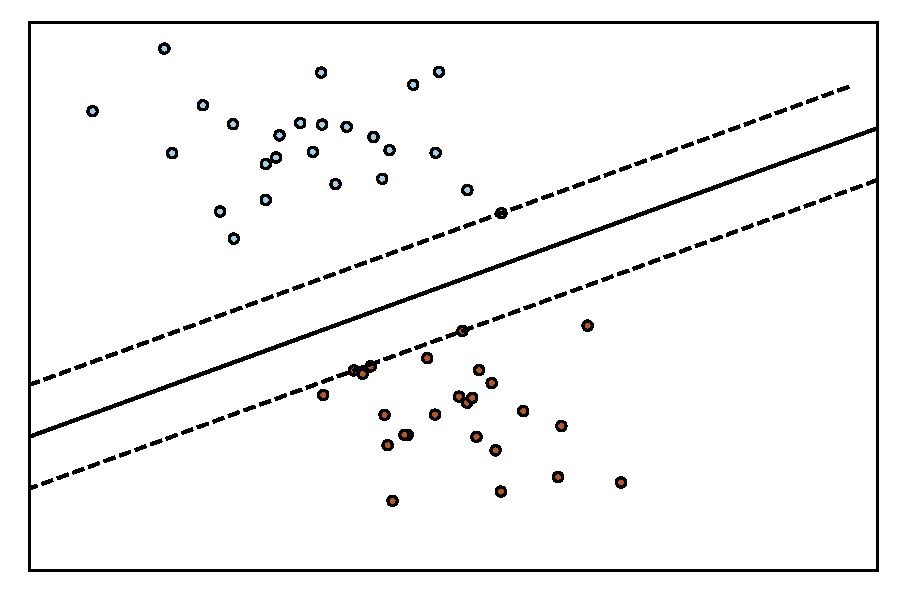
\includegraphics[width=\textwidth]{Chapter2/SeparableProblem/maxmargin_boundary.pdf}
                 \end{center}
            \end{column}
      \end{columns}
      % \begin{columns}
      %       \begin{column}{width=0.5\textwidth}
      %             \begin{itemize}
      %                   \item Las Máquinas de Vectores Soporte (SVM) son modelos populares
      %                   \item Tratan de maximizar
      %             \end{itemize}
      %       \end{column}
      %       \begin{column}{width=0.5\textwidth}
      %             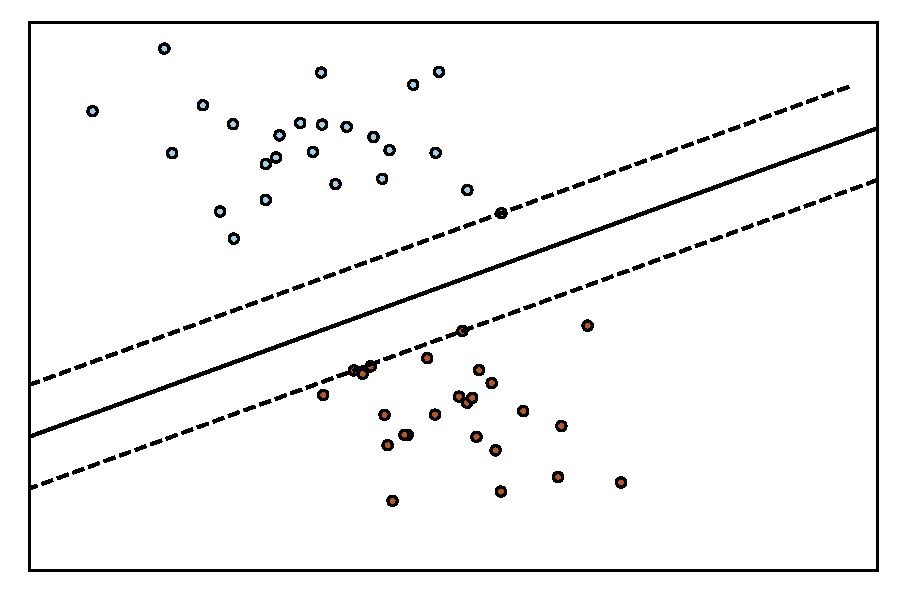
\includegraphics[width=0.6\textwidth]{Chapter2/SeparableProblem/maxmargin_boundary.pdf}
      %       \end{column}
      % \end{columns}

\end{frame}

\begin{frame}{L1-SVM}
      \begin{block}{Problema Primal - L1-SVM}
            \begin{myequation}
                  \nonumber
                  \begin{aligned}
                      &\min_{w, b, \fv{\xi}} & & C \sum_{i=1}^\nsamples \xi_i + \frac{1}{2} \norm{w}^2 \\
                      & \text{s.t.} & & y_i (\dotp{w}{\phi(x_i)} + b) \geq p_i - \xi_i , \\
                      & & & \xi_i \geq 0   
                  \end{aligned}  
              \end{myequation}
  \end{block}
  \begin{itemize}
      \item Se puede ver que esta formulación es equivalente a
      \begin{itemize}
          \item Máquina de Vectores Soporte para Clasificación (SVC): $p_i=1$ para $i=1, \ldots \nsamples$
          \item Máquina de Vectores Soporte para Regresión (SVR): se duplican los patrones
          \begin{itemize}
              \item $y_i = 1 , \; p_i = t_i - \epsilon$, en la primera mitad
              \item $y_{i} = -1 ,\; p_{i} = -t_i - \epsilon$, en la segunda mitad
          \end{itemize}
      \end{itemize}
  \end{itemize}
  
  \end{frame}


  \begin{frame}{L1-SVM}
      \begin{block}{Problema Dual - L1-SVM}
            \begin{myequation}
                  \nonumber %\label{eq:kernel_dual_matrix}
                  \begin{aligned}
                      &\min_{\fv{\alpha}} & & \frac{1}{2} \fv{\alpha}^\intercal \fm{Q} \fv{\alpha} - \fv{\alpha}^\intercal \fv{p} \\
                      & \text{s.t.} & & \sum_{i=1}^\nsamples y_i \alpha_i = 0 , \\
                      & & & 0 \leq \alpha_i \leq C    
                  \end{aligned}  
            \end{myequation}
      \end{block}
      \begin{itemize}
          \item Aquí $Q$ es la matriz de kernel 
          \begin{itemize}
              \item SVM lineal: $Q_{ij} = y_i y_j \dotp{x_i}{x_j} $
              \item SVM no lineal: $Q_{ij} = y_i y_j k(x_i, x_j) = y_i y_j \dotp{\phi({x_i})}{\phi({x_j})} $
          \end{itemize}
          
      \end{itemize}
          
  \end{frame}


  \begin{frame}{L2-SVM}
      \begin{block}{Problema Primal - L2-SVM}
            \begin{myequation}
                  \nonumber%\label{eq:l2_primal_clas}
                  \begin{aligned}
                      &\min_{w, b, \fv{\xi}} & & \frac{C}{2} \sum_{i=1}^m (\xi_i)^2 + \frac{1}{2} \norm{w}^2 \\
                      & \text{s.t.} & & y_i (\dotp{w}{\phi(x_i)} + b) \geq p_i - \xi_i 
                  \end{aligned}  
              \end{myequation}
      \end{block}

  \begin{block}{Problema Dual - L2-SVM}
      \begin{myequation}
            \nonumber%\label{eq:l2_dual_matrix}
            \begin{aligned}
                &\min_{\fv{\alpha}} & & \frac{1}{2} \fv{\alpha}^\intercal \left( \fm{Q} + \frac{1}{C} \fm{I}_\nsamples \right)\fv{\alpha} - \fv{\alpha}^\intercal \fv{p} \\
                & \text{s.t.} & & \sum_{i=1}^\nsamples y_i \alpha_i = 0 , \; \alpha_i \geq 0 
            \end{aligned}  
        \end{myequation}
\end{block}
  
  \end{frame}
  



\begin{frame}{LS-SVM}
      \begin{block}{Problema Primal - LS-SVM}
            \begin{myequation}
                  \nonumber%\label{eq:ls_primal}
                  \begin{aligned}
                      &\min_{w, b, \fv{\xi}} & & \frac{C}{2} \sum_{i=1}^\nsamples (\xi_i)^2 + \frac{1}{2} \norm{w}^2 \\
                      & \text{s.t.} & & y_i (\dotp{w}{x_i} + b) = p_i - \xi_i 
                  \end{aligned}  
              \end{myequation}
  \end{block}
  \begin{block}{Problema Dual - LS-SVM}
      \begin{myequation}\nonumber%\label{eq:ls_dual_matrix}
            \begin{aligned}
            \left[
            \begin{array}{c|c}
            0 & \fv{y}^\intercal \\
            \hline
            \fv{y} & \fm{Q} + \frac{1}{C} \fm{I}_\nsamples
            \end{array}
            \right] 
            \begin{bmatrix}
                b \\
                \fv{\alpha}
            \end{bmatrix}
            = 
            \begin{bmatrix}
                0 \\
                \fv{p}
            \end{bmatrix}
            \end{aligned}
        \end{myequation}
  \end{block}
  
\end{frame}

  

%%%%%%%%%%%%%%%%%%%%%%%%%%%%%%%%%%%%%%%%%%%%%%%%%%%%%%%%%%%%%%%%%%%%%%%%%%%%%%%%%%%%%%%
\section{Formulación Convexa para Aprendizaje Multitarea: Métodos de Kernel}

\subsection{Formulación Convexa con Métodos de Kernel}

\begin{frame}
    \frametitle{Formulación Aditiva con Métodos de Kernel}

    \begin{itemize}
        \item Una manera de implementar el MTL es combinar una parte común y otras específicas
      %   \item La formulación aditiva para el aprendizaje multitarea es
      %   \begin{myequation}
      %       \nonumber
      %       h_r(\cdot) = g(\cdot) + g_r(\cdot) 
      %   \end{myequation}
      %   donde
      %   \begin{itemize}
      %       \item $g(\cdot)$ es la parte común
      %       \item $g_r(\cdot)$ es la parte específica
      %   \end{itemize}
        \item Fue propuesta incialmente para SVM lineales en~\footfullcite{EvgeniouP04} con los modelos
        \begin{myequation}
            \nonumber
            h_r(\cdot) = \dotp{w + v_r}{\cdot} + b_r
        \end{myequation}
        y fue extendida al caso no lineal en~\footfullcite{CaiC09} con los modelos
        \begin{myequation}
            \nonumber
            h_r(\cdot) = \dotp{w}{\phi(\cdot)} + \dotp{{v}_r}{\phi_r(\cdot)} + b_r
      \end{myequation}
      donde $w$ es el parámetro de la parte común y $v_r$ los de las partes específicas
      % \begin{itemize}
      %       \item 
      %       \item $v_r$ son los parámetros de las partes específicas
      % \end{itemize}
    \end{itemize}
    
\end{frame}


\begin{frame}
      \frametitle{Formulación Aditiva para L1-SVM MT}
  
      \begin{block}{Problema Primal - L1-SVM MT Aditiva}
          \begin{myequation}\nonumber
              \begin{aligned}
              & \argmin_{w, \fv{v}, \fv{b}, \xi}
              & & { C \sum_{r= 1}^T \sum_{i=1}^{m_r} {\xi_{i}^r} + \frac{1}{2} \sum_{r= 1}^T{\norm{{v}_r}^2} + \frac{\mu}{2} {\norm{{w}}}^2} \\
              & \text{s.t.}
              & & y_{i}^r (\dotp{w}{\phi(x_{i}^r)} + \dotp{v_r}{\phi_r(x_{i}^r)} + b_r) \geq p_{i}^r - \xi_{i}^r ,  \\
              & & & \xi_{i}^r \geq 0; \;  i=1 , \dotsc , m_r, \;  r= 1,\dotsc, T  \\
              \end{aligned}
          \end{myequation}   
      \end{block}
      \begin{itemize}
          \item El parámetro $\mu$ (junto con $C$) regula la influencia de cada parte:
          \begin{itemize}
              \item $\mu \to \infty$: modelos independientes (ITL)
              \item $C \to 0,\; \mu \to 0$: modelo común (CTL)
          \end{itemize}
          \item Tenemos la transformación común $\phi$ y las específicas $\phi_r$ 
      \end{itemize}
  \end{frame}
  

\begin{frame}
      \frametitle{Formulacion Convexa con Métodos de Kernel}
  
      \begin{itemize}
          \item Proponemos~\footfullcite{RuizAD19} la siguiente formulación convexa para el aprendizaje multitarea:
          \begin{myequation}
            \nonumber
            h_r(\cdot) = \lambda_r \left\lbrace \dotp{w}{\phi(\cdot)} + b  \right\rbrace + (1 - \lambda_r) \left\lbrace \dotp{{v}_r}{\phi_r(\cdot)} + d_r \right\rbrace, \; \lambda_r \in [0,1]
      \end{myequation}
      %     \begin{myequation}
      %         \nonumber
      %         h_r(\cdot) = \lambda_r g(\cdot) + (1 - \lambda_r) g_r(\cdot) ,
      %     \end{myequation}
          % con $\lambda_r \in [0,1]$
          \item Los hiperparámetros $\lambda_r$, en lugar de $\mu$, regulan la influencia de cada parte
      %     \begin{itemize}
      %         \item $\lambda_1, \ldots, \lambda_\ntasks=0$: modelos independientes (ITL)
      %         \item $\lambda_1, \ldots, \lambda_\ntasks=1$: modelo común (CTL)
      %     \end{itemize}
          \item Extendemos esta formulación~\footfullcite{RuizAD21} y desarrollamos tres variantes de SVM:
          \begin{itemize}
                \item L1-SVM
                \item L2-SVM
                \item LS-SVM
          \end{itemize}
          %\item La interpretación de los hiperparámetros es más sencilla \\
            %\Mark{100}
      \end{itemize}
      
  \end{frame}



% \begin{frame}
%       \frametitle{Formulacion Convexa con Métodos de Kernel}

%       \begin{itemize}
%             \item La formulación aditiva de~\footfullcite{CaiC09} con métodos de kernel es:
%             \begin{myequation}
%                   \nonumber
%                   h_r(\cdot) = \left\lbrace \dotp{w}{\phi(\cdot)} + b  \right\rbrace + \left\lbrace \dotp{{v}_r}{\phi_r(\cdot)} + d_r \right\rbrace
%             \end{myequation}
%             \item En~\footfullcite{RuizAD19} proponemos la formulación convexa:
%             \begin{myequation}
%                   \nonumber
%                   h_r(\cdot) = \lambda_r \left\lbrace \dotp{w}{\phi(\cdot)} + b  \right\rbrace + (1 - \lambda_r) \left\lbrace \dotp{{v}_r}{\phi_r(\cdot)} + d_r \right\rbrace
%             \end{myequation}
%             \item Desarrollamos en~\footfullcite{RuizAD21} tres variantes de SVM:
%             \begin{itemize}
%                   \item L1-SVM
%                   \item L2-SVM
%                   \item LS-SVM
%             \end{itemize}
%       \end{itemize}

% \end{frame}



  
  
%   \begin{frame}
%         \frametitle{Formulación Aditiva para MTL L1-SVM}
    
%         \begin{block}{Problema Dual - L1-SVM Aditiva}
%               \begin{myequation}\nonumber
%                     \begin{aligned}
%                     & \min_{\fv{\alpha}} && \Theta(\fv{\alpha}) = \frac{1}{2} \fv{\alpha}^\intercal \left(\frac{1}{\mu} \fm{Q} + \fm{K} \right) \fv{\alpha} - \fv{p} \fv{\alpha} \\
%                     & \text{s.t.}
%                     & & 0 \leq \alpha_i^r \leq C ; \; i=1, \ldots, \npertask_r,\;\; r=1, \ldots, \ntasks ,\\
%                     & & & \sum_{i=1}^{m_r} \alpha_i^r y_i^r = 0;\;  r=1, \ldots, \ntasks . \\
%                     \end{aligned}
%                 \end{myequation}
%         \end{block}
%         \begin{itemize}
%             \item El parámetro $\mu$ (junto con $C$) regula la influencia de cada parte:
%             \begin{itemize}
%                 \item $\mu \to \infty$: modelos independientes (ITL)
%                 \item $C \to 0,\; \mu \to 0$: modelo común (CTL)
%             \end{itemize}
%         \end{itemize}
%     \end{frame}
  
  
  
  \begin{frame}
      \frametitle{Formulación Convexa para L1-SVM MT}
  
      \begin{block}{Problema Primal - L1-SVM MT Convexa}
            \begin{myequation}\nonumber
                  \begin{aligned}
                  & \min_{w, \fv{v}, b, \fv{d}, \fv{\xi}}
                  & & { C \sum_{r= 1}^T \sum_{i=1}^{m_r} {\xi_{i}^r} + \frac{1}{2} \sum_{r= 1}^T{\norm{{v}_r}^2} + \frac{1}{2} {\norm{{w}}}^2} \\
                  & \text{s.t.}
                  & & y_{i}^r \left(\lambda_r \left\lbrace \dotp{w}{\phi(x_{i}^r)} + b  \right\rbrace + (1 - \lambda_r) \left\lbrace \dotp{{v}_r}{\phi_r(x_{i}^r)} + d_r \right\rbrace  \right) \geq p_{i}^r - \xi_{i}^r ,  \\
                  & & & \xi_{i}^r \geq 0, \;  i=1 , \dotsc , m_r, \;  r= 1,\dotsc, T  \\
                  \end{aligned}
              \end{myequation}   
      \end{block}
      \begin{itemize}
            \item Los hiperparámetros $\lambda_r$ regulan la influencia de cada parte:
            \begin{itemize}
                \item $\lambda_1, \ldots, \lambda_\ntasks=0$: modelos independientes (ITL)
                \item $\lambda_1, \ldots, \lambda_\ntasks=1$: modelo común (CTL)
            \end{itemize}
            \item El hiperparámetro $C$ no interviene en el grado de interdependencia de los modelos
      \end{itemize}

  \end{frame}


  \begin{frame}
      \frametitle{Formulación Convexa para L1-SVM MT}
  
      \begin{block}{Problema Dual - L1-SVM MT Convexa}
            \begin{myequation}\nonumber
                  \begin{aligned}
                  & \min_{\fv{\alpha}} &&  \frac{1}{2} \fv{\alpha}^\intercal \left(\Lambda \fm{Q} \Lambda + \left(\fm{I}_{\nsamples} - \Lambda \right) \fm{K} \left(\fm{I}_{\nsamples} - \Lambda \right) \right) \fv{\alpha} - \fv{p} \fv{\alpha} \\
                  & \text{s.t.}
                  & & 0 \leq \alpha_i^r \leq C ; \; i=1, \ldots, \npertask_r,\; r=1, \ldots, \ntasks ,\\
                  & & & \sum_{i=1}^{m_r} \alpha_i^r y_i^r = 0;\;  r=1, \ldots, \ntasks \\
                  \end{aligned}
              \end{myequation}
            %   donde
            %   \begin{myequation}\nonumber
            %       \Lambda = \Diag(\overbrace{\lambda_1, \ldots, \lambda_1}^{\npertask_1}, \ldots, \overbrace{\lambda_\ntasks, \ldots, \lambda_\ntasks}^{\npertask_\ntasks})
            %   \end{myequation}
      \end{block}
      \begin{itemize}
            \item Usamos la matriz $  \Lambda = \Diag(\overbrace{\lambda_1, \ldots, \lambda_1}^{\npertask_1}, \ldots, \overbrace{\lambda_\ntasks, \ldots, \lambda_\ntasks}^{\npertask_\ntasks}) $
            \item La matriz $Q$ es común entre todas las tareas usando el kernel $k$ correspondiente a $\phi$
            \item La matriz $K$ es diagonal por bloques, con los kernel $k_r$ correspondientes a $\phi_r$
            \item La función de kernel es: 
            \begin{myequation}
                  \nonumber
                  \widehat{k}({x}_i^r, {x}_j^s) = \lambda_r \lambda_s k({x}_i^r, {x}_j^s) +  \delta_{rs} (1-\lambda_r) (1 - \lambda_s) k_r({x}_i^r, {x}_j^s) 
            \end{myequation}
      \end{itemize}

  \end{frame}



%   \begin{frame}
%       \frametitle{Formulación Convexa para L1-SVM MT}
  
%       \begin{block}{Problema Dual - L1-SVM Convexa ($\lambda$ común)}
%             \begin{myequation}\nonumber
%                   \begin{aligned}
%                   & \min_{\fv{\alpha}} && \Theta(\fv{\alpha}) = \frac{1}{2} \fv{\alpha}^\intercal \left(\lambda^2 \fm{Q} + \left( 1 - \lambda \right)^2 \fm{K}  \right) \fv{\alpha} - \fv{p} \fv{\alpha} \\
%                   & \text{s.t.}
%                   & & 0 \leq \alpha_i^r \leq C ; \; i=1, \ldots, \npertask_r,\; r=1, \ldots, \ntasks ,\\
%                   & & & \sum_{i=1}^{m_r} \alpha_i^r y_i^r = 0;\;  r=1, \ldots, \ntasks , \\
%                   \end{aligned}
%               \end{myequation}
%       \end{block}
%       \begin{itemize}
%             \item La función de kernel es: 
%             $$     \widehat{k}({x}_i^r, {x}_j^s) = \lambda^2 k({x}_i^r, {x}_j^s) +   (1-\lambda)^2 \delta_{rs} k_r({x}_i^r, {x}_j^s) 
%             $$
%             \item El hiperparámetro $\lambda$ regula la influencia de cada parte:
%             \begin{itemize}
%                 \item $\lambda=0$: modelos independientes (ITL)
%                 \item $\lambda=1$: modelo común (CTL)
%             \end{itemize}
%       \end{itemize}

%   \end{frame}


\begin{frame}
      \frametitle{Equivalencia}

      \begin{proposition}[Equivalencia entre formulaciones para L1-SVM MT]
            Para valores $\lambda \in (0, 1)$, la formulación aditiva con hiperparámetros $C_\text{add}, \mu$ y la formulación convexa con $C_\text{conv}$ y un $\lambda$ común, $\lambda_1, \ldots, \lambda_\ntasks = \lambda$, son equivalentes cuando
            \begin{myequation}
                  \nonumber
                  C_\text{add} = (1 - \lambda)^2 C_\text{conv}, \; \mu = (1 - \lambda)^2 / \lambda^2 .
            \end{myequation}
      \end{proposition}

      \begin{itemize}
            \item Para $\lambda = 0$, la formulación convexa con un $\lambda$ común es equivalente a modelos independientes (ITL)
            \item Para $\lambda = 1$, la formulación convexa con un $\lambda$ común es equivalente a un modelo común (CTL)
      \end{itemize}
     
      % \begin{proposition}[Equivalencia con CTL e ITL]
      %       \begin{itemize}
      %             \item Para $\lambda = 0$, la formulación convexa con un $\lambda$ común es equivalente a modelos independientes (ITL).
      %             \item Para $\lambda = 1$ la formulación convexa con un $\lambda$ común es equivalente a un modelo común (CTL).
      %       \end{itemize}
      % \end{proposition}

\end{frame}


\begin{frame}
      \frametitle{Formulación Aditiva vs. Formulación Convexa}

    

%       \centering
    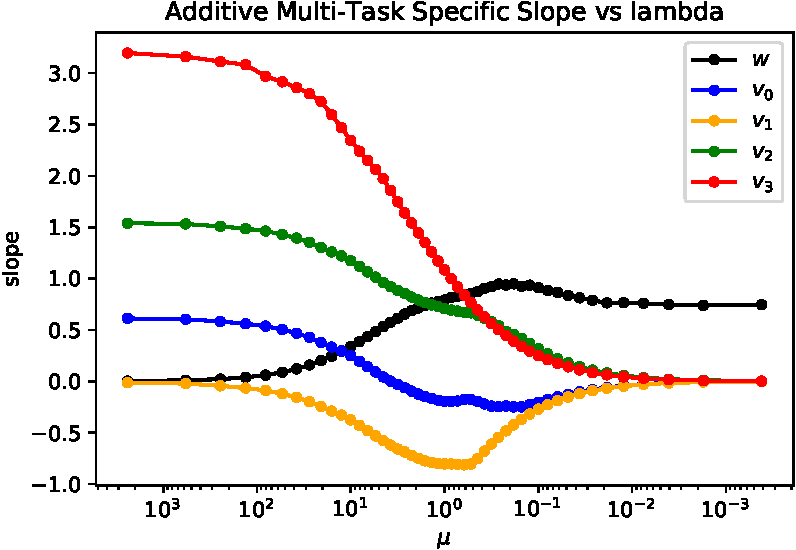
\includegraphics[width=.5\textwidth]{Chapter6/HAIS2019/synthetic_specWeights_add-crop.pdf}%
    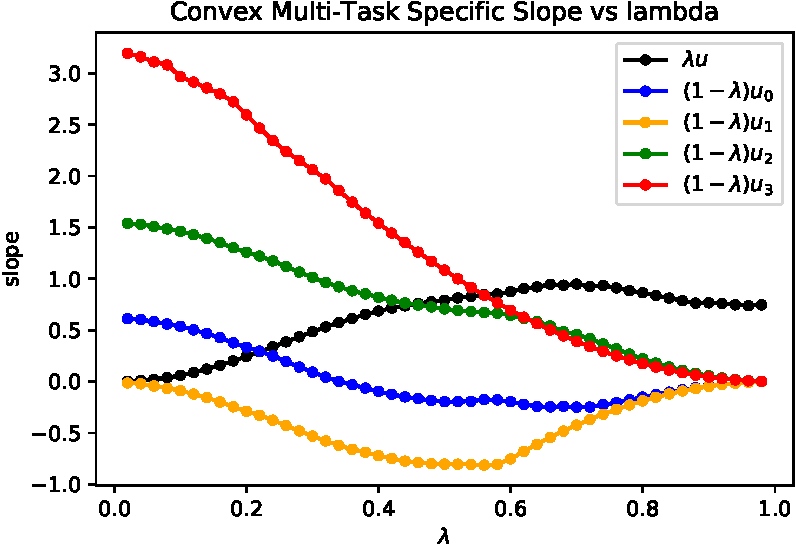
\includegraphics[width=.5\textwidth]{Chapter6/HAIS2019/synthetic_specWeights_conv-crop.pdf}%
%     \includegraphics[width=.5\textwidth]{synthetic_specWeights_conv.pdf}

    

\end{frame}



\begin{frame}
      \frametitle{Formulación Convexa para L2-SVM MT}

      \begin{block}{Problema Primal - L2-SVM MT Convexa}
            \begin{myequation}\nonumber
                  \begin{aligned}
                  & \argmin_{w, \fv{v}, b, \fv{d}, \xi}
                  & & {\frac{C}{2} \sum_{r= 1}^T \sum_{i=1}^{m_r} ({\xi_{i}^r})^2 + \frac{1}{2} \sum_{r= 1}^T{\norm{{v}_r}^2} + \frac{1}{2} {\norm{{w}}}^2} \\
                  & \text{s.t.}
                  & & y_{i}^r \left(\lambda_r \left\lbrace \dotp{w}{\phi(x_{i}^r)} + b  \right\rbrace + (1 - \lambda_r) \left\lbrace \dotp{{v}_r}{\phi_r(x_{i}^r)} + d_r \right\rbrace  \right) \geq p_{i}^r - \xi_{i}^r  \\
                  \end{aligned}
              \end{myequation}
      \end{block}

      \begin{block}{Problema Dual - L2-SVM MT Convexa}
            \begin{myequation}\nonumber
                  \begin{aligned}
                  & \min_{\fv{\alpha}} && \frac{1}{2} \fv{\alpha}^\intercal \left( \left\lbrace \Lambda \fm{Q} \Lambda + \left(\fm{I}_{\nsamples} - \Lambda \right) \fm{K} \left(\fm{I}_{\nsamples} - \Lambda \right) \right\rbrace + \frac{1}{C} \fm{I} \right) \fv{\alpha} - \fv{p} \fv{\alpha} \\
                  & \text{s.t.}
                  & & 0 \leq \alpha_i^r , \; i=1, \ldots, \npertask_r,\; r=1, \ldots, \ntasks, \\
                  & & & \sum_{i=1}^{m_r} \alpha_i^r y_i^r = 0, \;  r=1, \ldots, \ntasks  \\
                  \end{aligned}
              \end{myequation}
      \end{block}
      

\end{frame}


% \begin{frame}
%       \frametitle{Extensiones a L2 y LS-SVM}

%       \begin{itemize}
%             \item En la SVM (L1-SVM) hemos definido los modelos:
%             \begin{myequation}
%                   \nonumber
%                   h_r(\cdot) = \lambda_r \left\lbrace \dotp{w}{\phi(\cdot)} + b  \right\rbrace + (1 - \lambda_r) \left\lbrace \dotp{{v}_r}{\phi_r(\cdot)} + d_r \right\rbrace
%             \end{myequation}
%       \end{itemize}

% \end{frame}


% \begin{frame}
%       \frametitle{Formulación Convexa para L2-SVM MT}
  
%       \begin{block}{Problema Dual - L2-SVM MT Convexa}
%             \begin{myequation}\nonumber
%                   \begin{aligned}
%                   & \min_{\alpha} && \Theta(\alpha) = \frac{1}{2} \fv{\alpha}^\intercal \left( \left\lbrace \Lambda \fm{Q} \Lambda + \left(\fm{I}_{\nsamples} - \Lambda \right) \fm{K} \left(\fm{I}_{\nsamples} - \Lambda \right) \right\rbrace + \frac{1}{C} \fm{I} \right) \fv{\alpha} - \fv{p} \fv{\alpha} \\
%                   & \text{s.t.}
%                   & & 0 \leq \alpha_i^r , \; i=1, \ldots, \npertask_r,\; r=1, \ldots, \ntasks, \\
%                   & & & \sum_{i=1}^{m_r} \alpha_i^r y_i^r = 0, \;  r=1, \ldots, \ntasks . \\
%                   \end{aligned}
%               \end{myequation}
%       \end{block}

%   \end{frame}


  \begin{frame}
      \frametitle{Formulación Convexa para LS-SVM MT}

      \begin{block}{Problema Primal - LS-SVM MT Convexa}
            \begin{myequation}\nonumber
                  \begin{aligned}
                  & \argmin_{w, \fv{v}, b, \fv{d}, \xi}
                  & & {\frac{C}{2} \sum_{r= 1}^T \sum_{i=1}^{m_r} \left({\xi_{i}^r}\right)^2 + \frac{1}{2} \sum_{r= 1}^T{\norm{{v}_r}^2} + \frac{1}{2} {\norm{{w}}}^2} \\
                  & \text{s.t.}
                  & & y_{i}^r \left(\lambda_r \left\lbrace \dotp{w}{\phi(x_{i}^r)} + b  \right\rbrace + (1 - \lambda_r) \left\lbrace \dotp{{v}_r}{\phi_r(x_{i}^r)} + d_r \right\rbrace  \right) = p_{i}^r - \xi_{i}^r   \\
                  \end{aligned}
              \end{myequation}
      \end{block}

      \begin{block}{Problema Dual - LS-SVM MT Convexa}
            \begin{myequation}
                  \nonumber
                  \begin{aligned}
                  \left[
                  \begin{array}{c|c|c}
                  0 & \fv{0}_\ntasks^\intercal &  \fv{y}^\intercal \Lambda \\
                  \hline
                  \fv{0}_\ntasks & \fv{0}_{\ntasks \times \ntasks} & \fm{A}^\intercal \fm{y} (I_\nsamples - \Lambda)\\
                  \hline
                  \fv{y} & \fm{y} \fm{A} & \left\lbrace \Lambda \fm{Q} \Lambda + \left(\fm{I}_{\nsamples} - \Lambda \right) \fm{K} \left(\fm{I}_{\nsamples} - \Lambda \right) \right\rbrace + \frac{1}{C} \fm{I} 
                  \end{array}
                  \right] 
                  \begin{pmatrix}
                      b \\
                      d_1 \\
                      \vdots \\
                      d_\ntasks \\
                      \fv{\alpha}
                  \end{pmatrix}
                  = 
                  \begin{pmatrix}
                      0 \\
                      \fv{0}_\ntasks \\
                      \fv{p}
                  \end{pmatrix}
                  \end{aligned}
              \end{myequation}
      \end{block}

\end{frame}










% \begin{frame}
%       \frametitle{Formulación Convexa para LS-SVM MT}
  
%       \begin{block}{Problema Dual - LS-SVM MT Convexa}
%             \begin{myequation}
%                   \nonumber
%                   \begin{aligned}
%                   \left[
%                   \begin{array}{c|c|c}
%                   0 & \fv{0}_\ntasks^\intercal &  \fv{y}^\intercal \Lambda \\
%                   \hline
%                   \fv{0}_\ntasks & \fv{0}_{\ntasks \times \ntasks} & \fm{A}^\intercal \fm{y} (I_\nsamples - \Lambda)\\
%                   \hline
%                   \fv{y} & \fm{y} \fm{A} & \widehat{\fm{Q}} + \frac{1}{C} \fm{I}_\nsamples
%                   \end{array}
%                   \right] 
%                   \begin{pmatrix}
%                       b \\
%                       d_1 \\
%                       \vdots \\
%                       d_\ntasks \\
%                       \fv{\alpha}
%                   \end{pmatrix}
%                   = 
%                   \begin{pmatrix}
%                       0 \\
%                       \fv{0}_\ntasks \\
%                       \fv{p}
%                   \end{pmatrix}, 
%                   \end{aligned}
%               \end{myequation}
%       \end{block}

%   \end{frame}



  


\subsection{Combinación Convexa de Modelos Preentrenados}

\begin{frame}
      \frametitle{Combinación Convexa de Modelos Preentrenados}

      \begin{itemize}
            \item Como alternativa natural, consideramos~\footfullcite{RuizAD21} la combinación convexa de
            \begin{itemize}
                  \item modelo común $g(\cdot)$ ya entrenado
                  \item modelos específicos $g_r(\cdot)$ ya entrenados
            \end{itemize}
            frente al aprendizaje MT con formulación convexa
            \item Minimizamos el riesgo eligiendo los hiperparámetros $\lambda_1, \ldots, \lambda_\ntasks$ óptimos
            \begin{myequation}
                  \nonumber
                  \emprisk(\lambda_1, \ldots, \lambda_\ntasks) = \sum_{r=1}^\ntasks \sum_{i=1}^{\npertask_r} \lossf(\lambda_r g(x_i^r) + (1 - \lambda_r) g_r(x_i^r), y_i^r) ,
              \end{myequation}
            \item Consideramos las pérdidas:
            \begin{itemize}
                  \item Cuadrática y Absoluta (regresión)
                  \item Hinge y Hinge Cuadrática (clasificación)
            \end{itemize}
      \end{itemize}

\end{frame}



% \begin{frame}
%       \frametitle{Formulación Unificada Clasificación}

%       \begin{itemize}
%             \item Hinge loss (classification):
%             \begin{myequation}
%                 \nonumber%\label{eq:hingeloss_emprisk}
%                 \emprisk(\lambda_1, \ldots, \lambda_\ntasks) = \sum_{r=1}^\ntasks \sum_{i=1}^{\npertask_r} \pospart{1 - y_i^r \left\lbrace\lambda_r g(x_i^r) + (1 - \lambda_r) g_r(x_i^r) \right \rbrace} .
%             \end{myequation}
%             \item Squared hinge loss (classification):
%             \begin{myequation}
%                 \nonumber%\label{eq:sqhingeloss_emprisk}
%                 \emprisk(\lambda_1, \ldots, \lambda_\ntasks) = \sum_{r=1}^\ntasks \sum_{i=1}^{\npertask_r} \pospart{1 - y_i^r \left\lbrace\lambda_r g(x_i^r) + (1 - \lambda_r) g_r(x_i^r) \right \rbrace}^2 .
%             \end{myequation}
%             \item Ambas se pueden expresar como:
%             \begin{myequation}
%                   \nonumber
%                   \sum_{r=1}^\ntasks \sum_{i=1}^{\npertask_r} u(\lambda_r c_i^r + d_i^r) , \; \text{donde} \; c_i^r =  y_i^r (g_r(x_i^r) - g(x_i^r))  , \;  d_i^r =  1 - y_i^r g_r(x_i^r)
%               \end{myequation}
%             %   donde
%             %   \begin{myequation}
%             %       \label{eq:changevar_clas}
%             %       c_i^r =  y_i^r (g_r(x_i^r) - g(x_i^r))  , \;  d_i^r =  1 - y_i^r g_r(x_i^r) ,
%             %   \end{myequation}
%         \end{itemize}

% \end{frame}


% \begin{frame}
%       \frametitle{Formulación Unificada Regresión}

%       \begin{itemize}
%             \item Absolute loss (regression):
%             \begin{myequation}
%                 \nonumber%\label{eq:absloss_emprisk}
%                 \emprisk(\lambda_1, \ldots, \lambda_\ntasks) = \sum_{r=1}^\ntasks \sum_{i=1}^{\npertask_r} \abs{y_i^r - \left\lbrace\lambda_r g(x_i^r) + (1 - \lambda_r) g_r(x_i^r) \right \rbrace} .
%             \end{myequation}
%             \item Squared loss (regression):
%             \begin{myequation}
%                 \nonumber%\label{eq:sqloss_emprisk}
%                 \emprisk(\lambda_1, \ldots, \lambda_\ntasks) = \sum_{r=1}^\ntasks \sum_{i=1}^{\npertask_r} \left( {y_i^r - \left\lbrace\lambda_r g(x_i^r) + (1 - \lambda_r) g_r(x_i^r) \right \rbrace} \right)^2 .
%             \end{myequation}
%             \item Ambas se pueden expresar como:
%             \begin{myequation}
%                   \nonumber
%                   \sum_{r=1}^\ntasks \sum_{i=1}^{\npertask_r} u(\lambda_r c_i^r + d_i^r) ,\; \text{donde} \; c_i^r = g(x_i^r) - g_r(x_i^r)  , \;  d_i^r =  g_r(x_i^r) - y_i^r
%               \end{myequation}
%             % donde $c_i^r = g(x_i^r) - g_r(x_i^r)  , \;  d_i^r =  g_r(x_i^r) - y_i^r .$
%             %   \begin{myequation}
%             %       \label{eq:changevar_reg}
%             %       c_i^r = g(x_i^r) - g_r(x_i^r)  , \;  d_i^r =  g_r(x_i^r) - y_i^r .
%             %   \end{myequation}
%         \end{itemize}

% \end{frame}

\begin{frame}
      \frametitle{Formulación Unificada}

      \begin{itemize}
            \item En todos los casos el riesgo lo podemos expresar como
            \begin{myequation}
                  \nonumber
                  \emprisk(\lambda_1, \ldots, \lambda_\ntasks) =
                  \sum_{r=1}^\ntasks \sum_{i=1}^{\npertask_r} u(\lambda_r c_i^r + d_i^r)
            \end{myequation}
            \item Como $\emprisk(\lambda_1, \ldots, \lambda_\ntasks)$ es separable, tenemos en cada tarea el problema
            \begin{myequation}
                  \nonumber
                  \argmin_{\lambda_r \in [0, 1]} \mathcal{J}(\lambda_r) = \sum_{i=1}^{\npertask_r} u(\lambda_r c_i^r + d_i^r)
            \end{myequation}
            \item Usando el Teorema de Fermat
            \begin{myequation}
                  \nonumber
                  \lambda^* = \argmin_{0 \leq \lambda \leq 1} \mathcal{J}(\lambda) \iff (0 \in \partial \mathcal{J}(\lambda^*) \text{ y } \lambda^* \in (0, 1) ) \text{ o } \lambda^*=0 \text{ o } \lambda^*=1 
              \end{myequation}
      \end{itemize}

\end{frame}


\begin{frame}
      \frametitle{Combinación Convexa con Error Cuadrático}

      \begin{itemize}
            \item La función a minimizar es 
            \begin{myequation}
                  \nonumber
                  %\label{eq:opt_sq}
                  \argmin_{\lambda \in [0, 1]} \mathcal{J}(\lambda) = \sum_{i=1}^{\npertask} \left({\lambda c_i + d_i}\right)^2 
            \end{myequation}
            \item La derivada es
            \begin{myequation}
                  \nonumber
                  \mathcal{J}'(\lambda) = \sum_{i=1}^\npertask 2 c_i (\lambda c_i + d_i) 
            \end{myequation}
            \item Como es derivable, resolviendo $\mathcal{J}'(\lambda)= 0$ obtenemos
            \begin{myequation*}
                  \lambda' =  -\frac{\sum_{i=1}^{\npertask} d_i c_i }{\sum_{i=1}^{\npertask} (c_i)^2 } 
                  \end{myequation*}
            \item La solución es entonces $\opt{\lambda} = \max(\min(\lambda', 1), 0)$
      \end{itemize}
        %
        
\end{frame}


% \begin{frame}

%       \begin{figure}[t!]
%             \centering
%             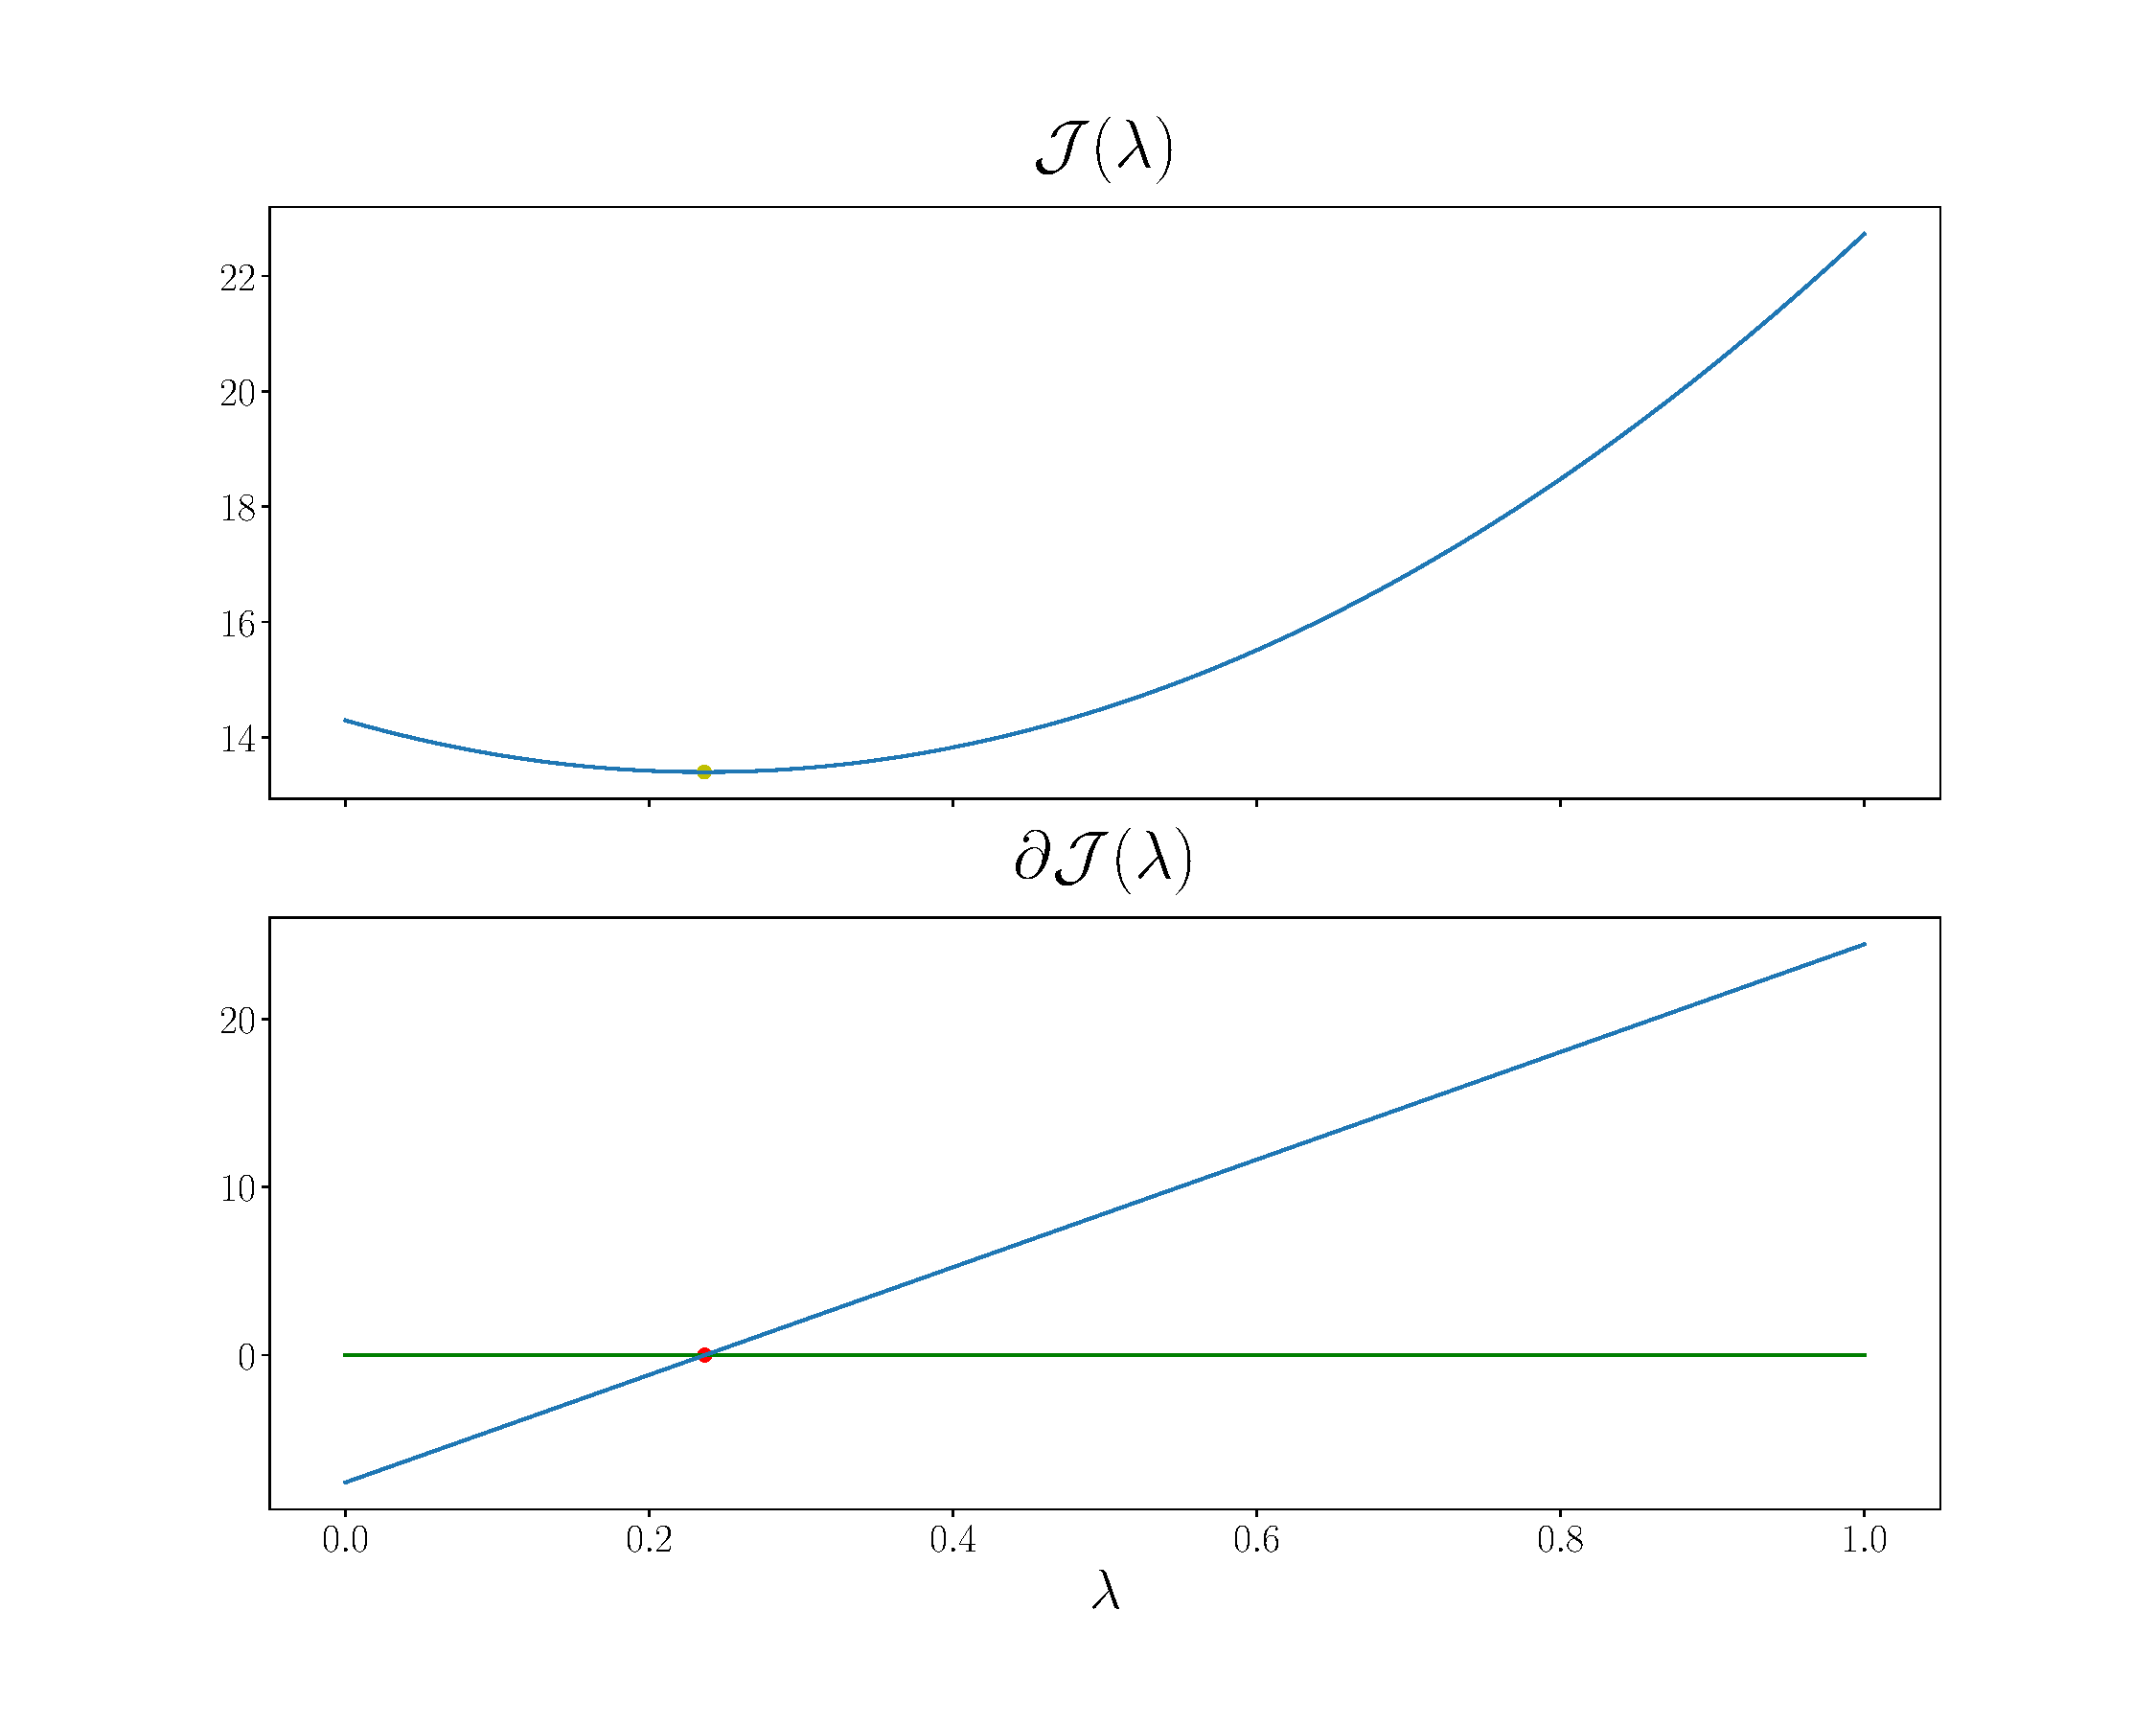
\includegraphics[width=.6\textwidth]{Chapter4/NeuroCom2021/ejemplo2_mse.pdf}
%             \caption{Error using the squared loss function (top) and its corresponding derivative (bottom). The green line represents the $0$ constant function. The yellow dot is the point minimizing the error, and whose corresponding derivative contains the value $0$.}
%             \label{fig:sq_error}
%         \end{figure}      

% \end{frame}

\begin{frame}      
      \frametitle{Combinación Convexa con Error Absoluto}


      \begin{columns}
            \begin{column}{0.5\textwidth}
                  \begin{itemize}
                        \item Hay que resolver
                        \begin{myequation}
                              \nonumber %\label{eq:opt_abs}
                              \argmin_{\lambda \in [0, 1]} \mathcal{J}(\lambda) = \sum_{i=1}^{\npertask} \abs{\lambda c_i + d_i}
                          \end{myequation}
                          \item El subgradiente de cada sumando es
                          \begin{myequation}
                              \nonumber %\label{eq:subdiff_abs}
                              \begin{aligned}
                                  \partial \abs{\lambda c_i + d_i} = 
                              \begin{cases}
                                  -\abs{c_i} ,& \lambda c_i + d_i  < 0, \\
                                  [-\abs{c_i}, \abs{c_i}] ,& \lambda c_i + d_i  = 0, \\
                                  \abs{c_i} ,& \lambda c_i + d_i  > 0 \\
                              \end{cases}
                              \end{aligned}
                          \end{myequation}
                  \end{itemize}
            \end{column}
            \begin{column}{0.5\textwidth}
                  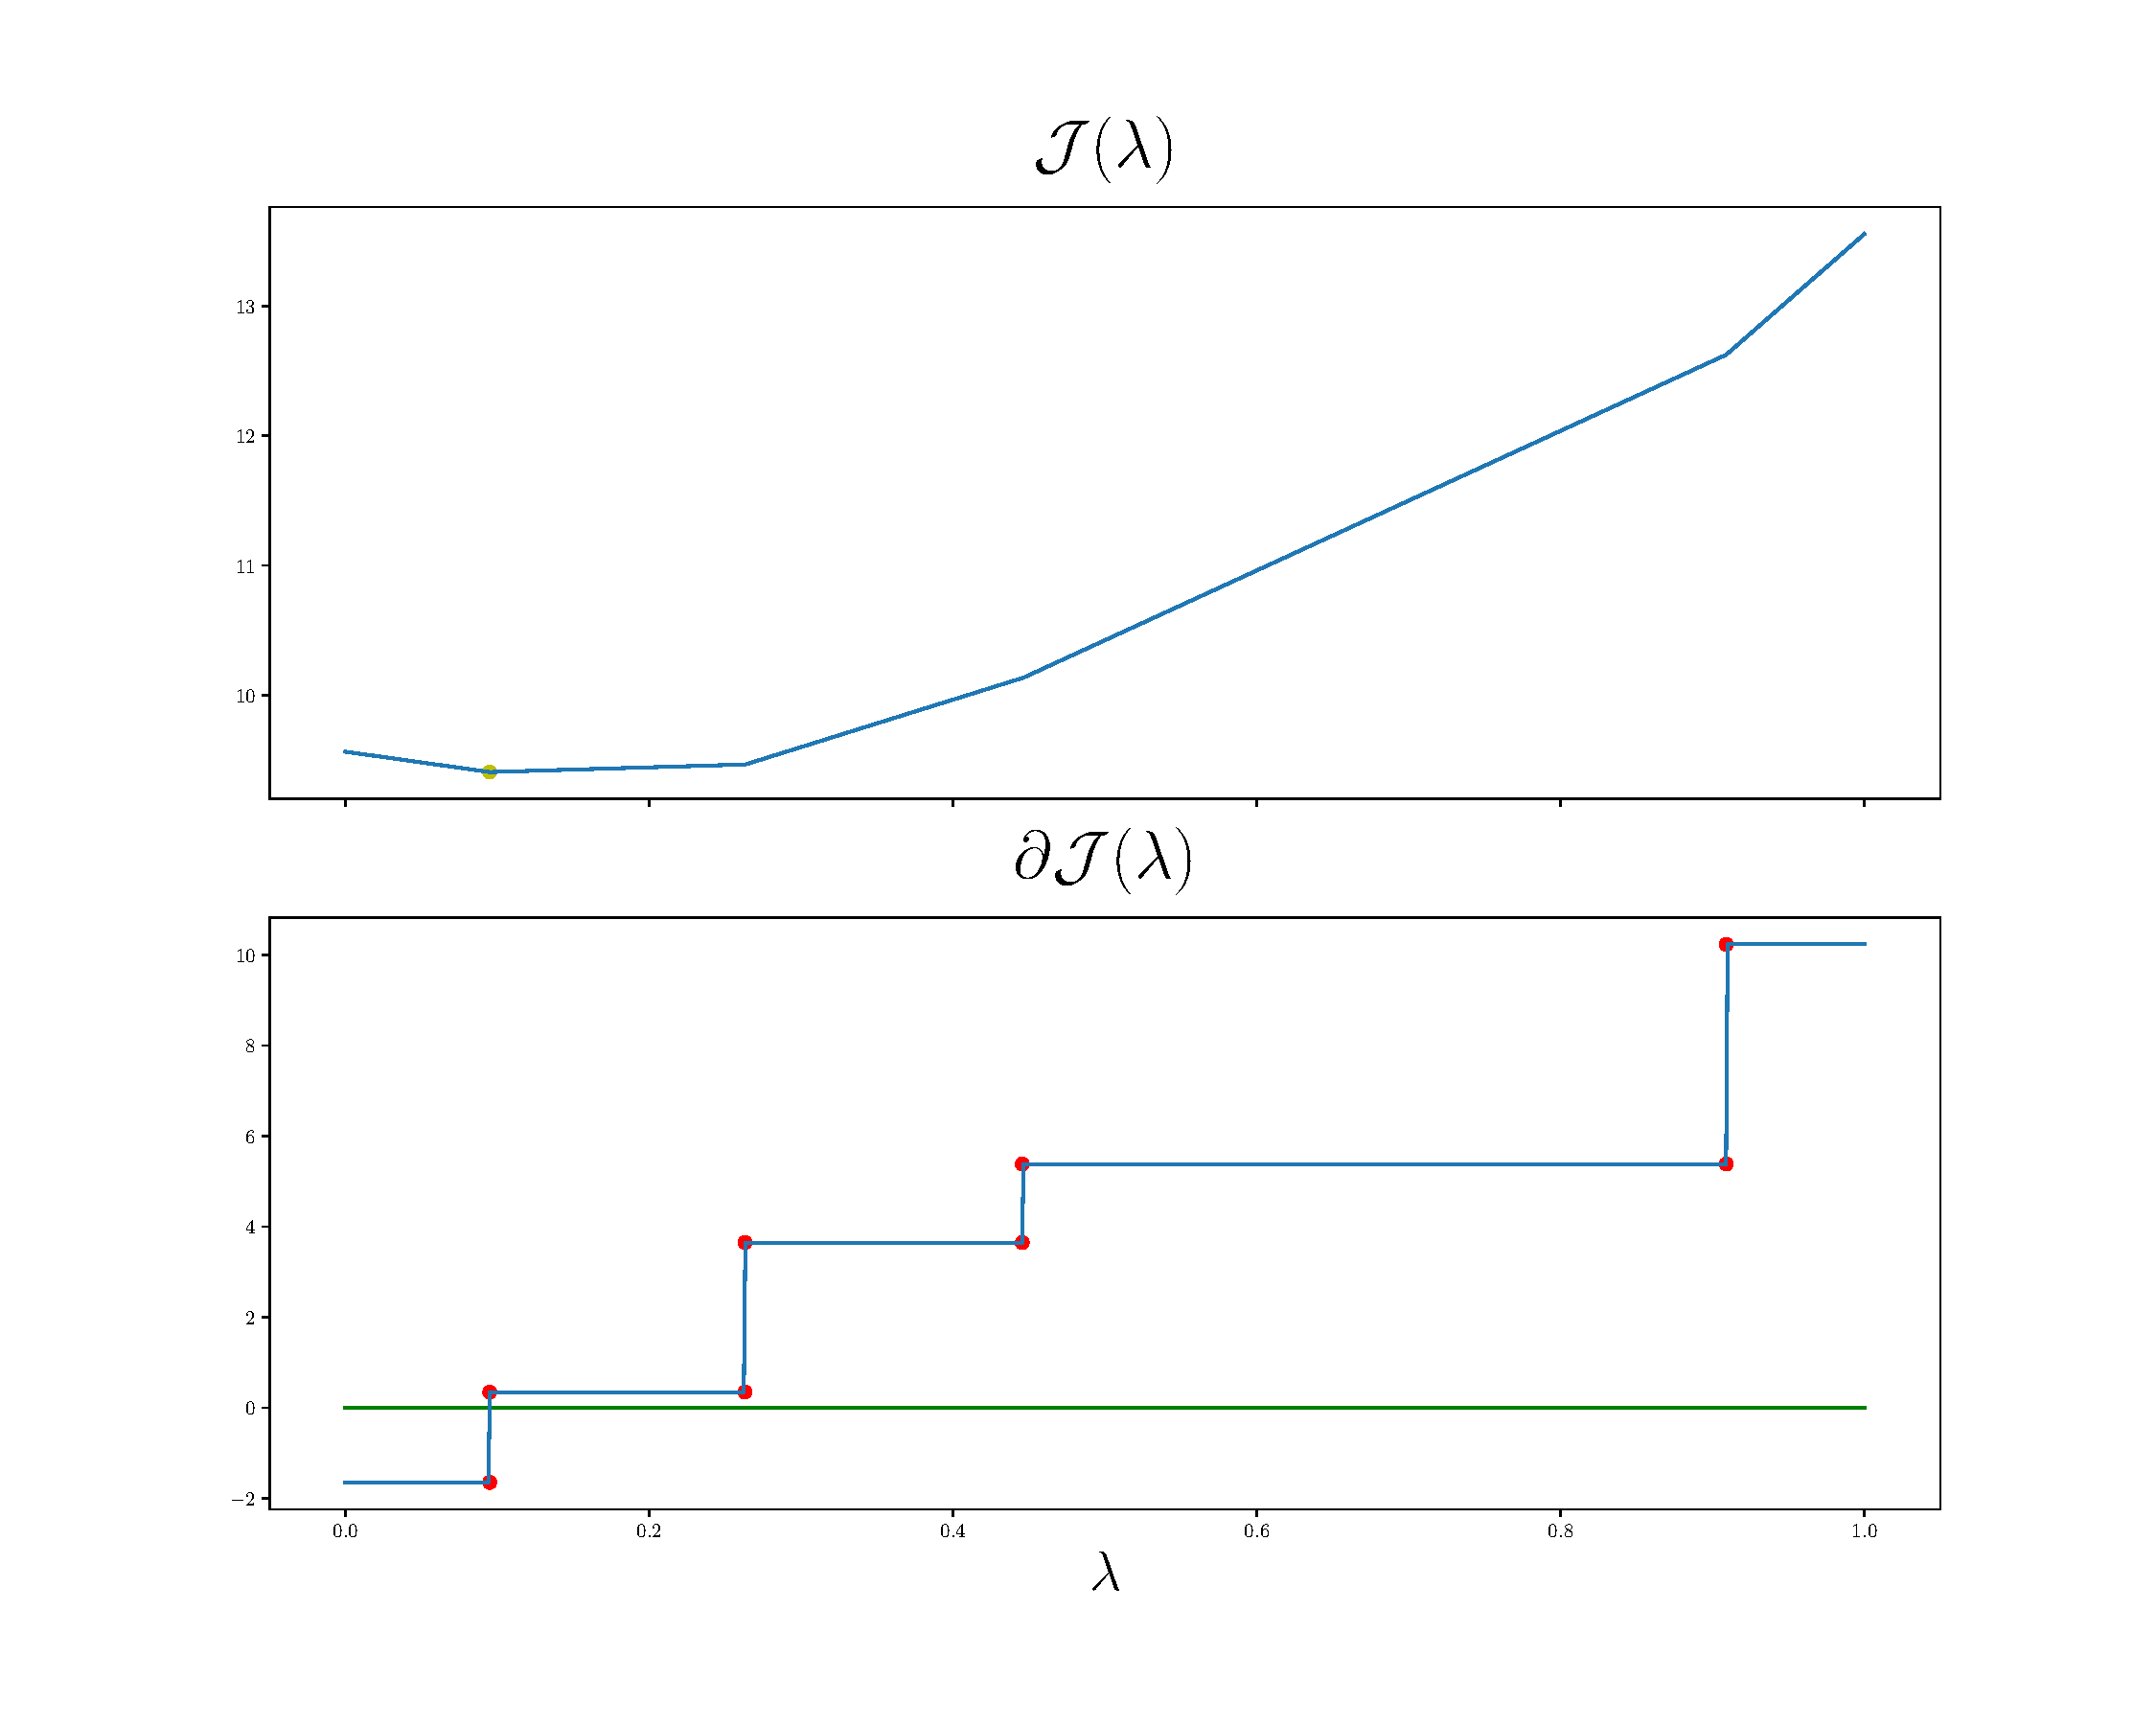
\includegraphics[width=\textwidth]{Chapter4/NeuroCom2021/ejemplo2_mae.pdf}
            \end{column}
      \end{columns}

\end{frame}

\begin{frame}
      \frametitle{Combinación Convexa con Error Absoluto}

      \begin{proposition}[$\lambda^*$ óptimo para el problema con valor absoluto]\label{prop:abs_neurocom2020}
            \begin{itemize}
                  \item $\lambda^*=0$ es óptimo si y solo si: $- \sum_{i: \; 0 > \lambda_{(i)}} \abs{c_{(i)}} + \sum_{i: \; 0 < \lambda_{(i)}} \abs{c_{(i)}} \leq 0$
                  \item $\lambda^* \in (0,1)$ es óptimo si y solo si $0 < \lambda^* = \lambda_{(k)} < 1$ para algún $k=1, \dotsc, \npertask$, y
                  \begin{myequation}
                  \nonumber    
                  - \sum_{i:\; \lambda_{(k)} > \lambda_{(i)}} \abs{c_{(i)}} + \sum_{i:\; \lambda_{(k)} < \lambda_{(i)}} \abs{c_{(i)}} \in \left[ -  \abs{c_{(k)}},  \abs{c_{(k)}}  \right] 
                  \end{myequation}
                  \item $\lambda^*=1$ es óptimo en otro caso
            \end{itemize}
        \end{proposition}
\end{frame}



\begin{frame}
      \frametitle{Combinación Convexa: Tabla}

      \begin{table}[t]
            \centering
            \scalebox{.7}{
             \begin{tabular}{c|c}
               \toprule
               \fhead{} & \fhead{$\opt{\lambda} \in (0, 1)$}  \\
               \midrule
             Cuadrática & $ 0 < -\frac{\sum_{i=1}^{\npertask} d_i c_i }{\sum_{i=1}^{\npertask} (c_i)^2 } < 1$ \\   
             \midrule
               Absoluta & $- \sum_{i:\; \lambda_{(k)} > \lambda_{(i)}} \abs{c_{(i)}} + \sum_{i:\; \lambda_{(k)} < \lambda_{(i)}} \abs{c_{(i)}} \in \left[ -  \abs{c_{(k)}},  \abs{c_{(k)}}  \right] $   \\ 
               \midrule
               Hinge & $-\sum_{i:\; \lambda_{(k)} > \lambda_{(i)}} \mymax{0, c_{(i)}} - \sum_{i:\; \lambda_{(k)} <\lambda_{(i)}} \mymin{0, c_{(i)}} \in \left[\mymin{0, c_{(k)}}, \mymax{0, c_{(k)}} \right]  $   \\ 
               \midrule
               Hinge Cuad. & $  - \frac{\sum_{i:\; \lambda_{(k+1)} \geq \lambda_{(i)}} \mymax{0, c_{(i)}} d_{(i)} + \sum_{i:\; \lambda_{(k)} \leq \lambda_{(i)}} \mymin{0, c_{(i)}} d_{(i)}}{\sum_{i:\; \lambda_{(k+1)} \geq \lambda_{(i)}} \mymax{0, c_{(i)}}^2 + \sum_{i:\; \lambda_{(k)} \leq \lambda_{(i)}} \mymin{0, c_{(i)}}^2} \in [\lambda_{(k)}, \lambda_{(k+1)}]  $   \\ 
               \toprule
             \fhead{} & \fhead{$\opt{\lambda}=0$}  \\
             \midrule
             Cuadrática & $ -\frac{\sum_{i=1}^{\npertask} d_i c_i }{\sum_{i=1}^{\npertask} (c_i)^2 } \leq 0$ \\             
              \midrule
               Absoluta & $- \sum_{i: \; 0 > \lambda_{(i)}} \abs{c_{(i)}} + \sum_{i: \; 0 < \lambda_{(i)}} \abs{c_{(i)}} \leq 0$   \\ 
               \midrule
               Hinge & $-\sum_{i:\; 0 > \lambda_{(i)}} \mymax{0, c_{(i)}} - \sum_{0 < \lambda_{(i)}} \mymin{0, c_{(i)}} \leq 0 $    \\ 
               \midrule
               Hinge Cuad. & $-\sum_{i:\; 0 > c_{(i)}, 0 < \lambda_{(i)}} {2 c_i d_i} - \sum_{i:\; 0 < c_{(i)}, 0 > \lambda_{(i)}} {2 c_{(i)} d_{(i)}}  \leq 0 $ \\ 
               \toprule
             \fhead{} & \fhead{$\opt{\lambda}=1$ en otro caso}  \\
               \bottomrule
             \end{tabular}
             }
        \end{table}
\end{frame}







% \begin{frame}
%       \frametitle{Combinación Convexa con Error Hinge}
%       \begin{proposition}[$\lambda^*$ óptimo para el problema con error hinge]\label{prop:hinge_neurocom2020}
%             \begin{itemize}
%                   \item $\lambda^*=0$ es óptimo si y solo si: $-\sum_{i:\; 0 > \lambda_{(i)}} \mymax{0, c_{(i)}} - \sum_{0 < \lambda_{(i)}} \mymin{0, c_{(i)}} \leq 0 $
%                   \item $\lambda^* \in (0,1)$ es óptimo si y solo si $0 < \lambda^* = \lambda_{(k)} < 1$ para algún $k=1, \dotsc, \npertask$, y
%                   \begin{myequation}
%                         \nonumber%\label{eq:sol_hinge}
%                         -\sum_{i:\; \lambda_{(k)} > \lambda_{(i)}} \mymax{0, c_{(i)}} - \sum_{i:\; \lambda_{(k)} <\lambda_{(i)}} \mymin{0, c_{(i)}} \in \left[\mymin{0, c_{(k)}}, \mymax{0, c_{(k)}} \right] 
%                   \end{myequation}
%                   \item $\lambda^*=1$ es óptimo en otro caso
%             \end{itemize}
%         \end{proposition}
%       % \begin{proposition}[Optimal $\lambda^*$ with Hinge Loss]\label{prop:hinge_neurocom2020}
%       %       In~\eqref{eq:opt_hinge_l1}, $\lambda^*=0$ is optimal iff
%       %       \begin{myequation}
%       %           \nonumber
%       %           %\label{eq:sol_hinge_0}
%       %           -\sum_{i:\; 0 > \lambda_{(i)}} \mymax{0, c_{(i)}} - \sum_{0 < \lambda_{(i)}} \mymin{0, c_{(i)}} \leq 0 .
%       %           \end{myequation}
%       %           If this condition does not hold, a value $\lambda^* \in (0, 1)$ is optimal for problem~\eqref{eq:opt_hinge_l1} \emph{iff} $\lambda^*$ is a feasible elbow, that is, $0 < \lambda^* = \lambda_{(k)} < 1$ for some $k=1, \dotsc, \npertask$, and
%       %       \begin{myequation}
%       %           \label{eq:sol_hinge}
%       %           -\sum_{i:\; \lambda_{(k)} > \lambda_{(i)}} \mymax{0, c_{(i)}} - \sum_{i:\; \lambda_{(k)} <\lambda_{(i)}} \mymin{0, c_{(i)}} \in \left[\mymin{0, c_{(k)}}, \mymax{0, c_{(k)}} \right] .
%       %       \end{myequation}
%       %       If none of the previous conditions hold, then $\lambda^*=1$ is optimal.
%       %   \end{proposition}
% \end{frame}


% % \begin{frame}

% %       \begin{figure}[t!]
% %             \centering
% %             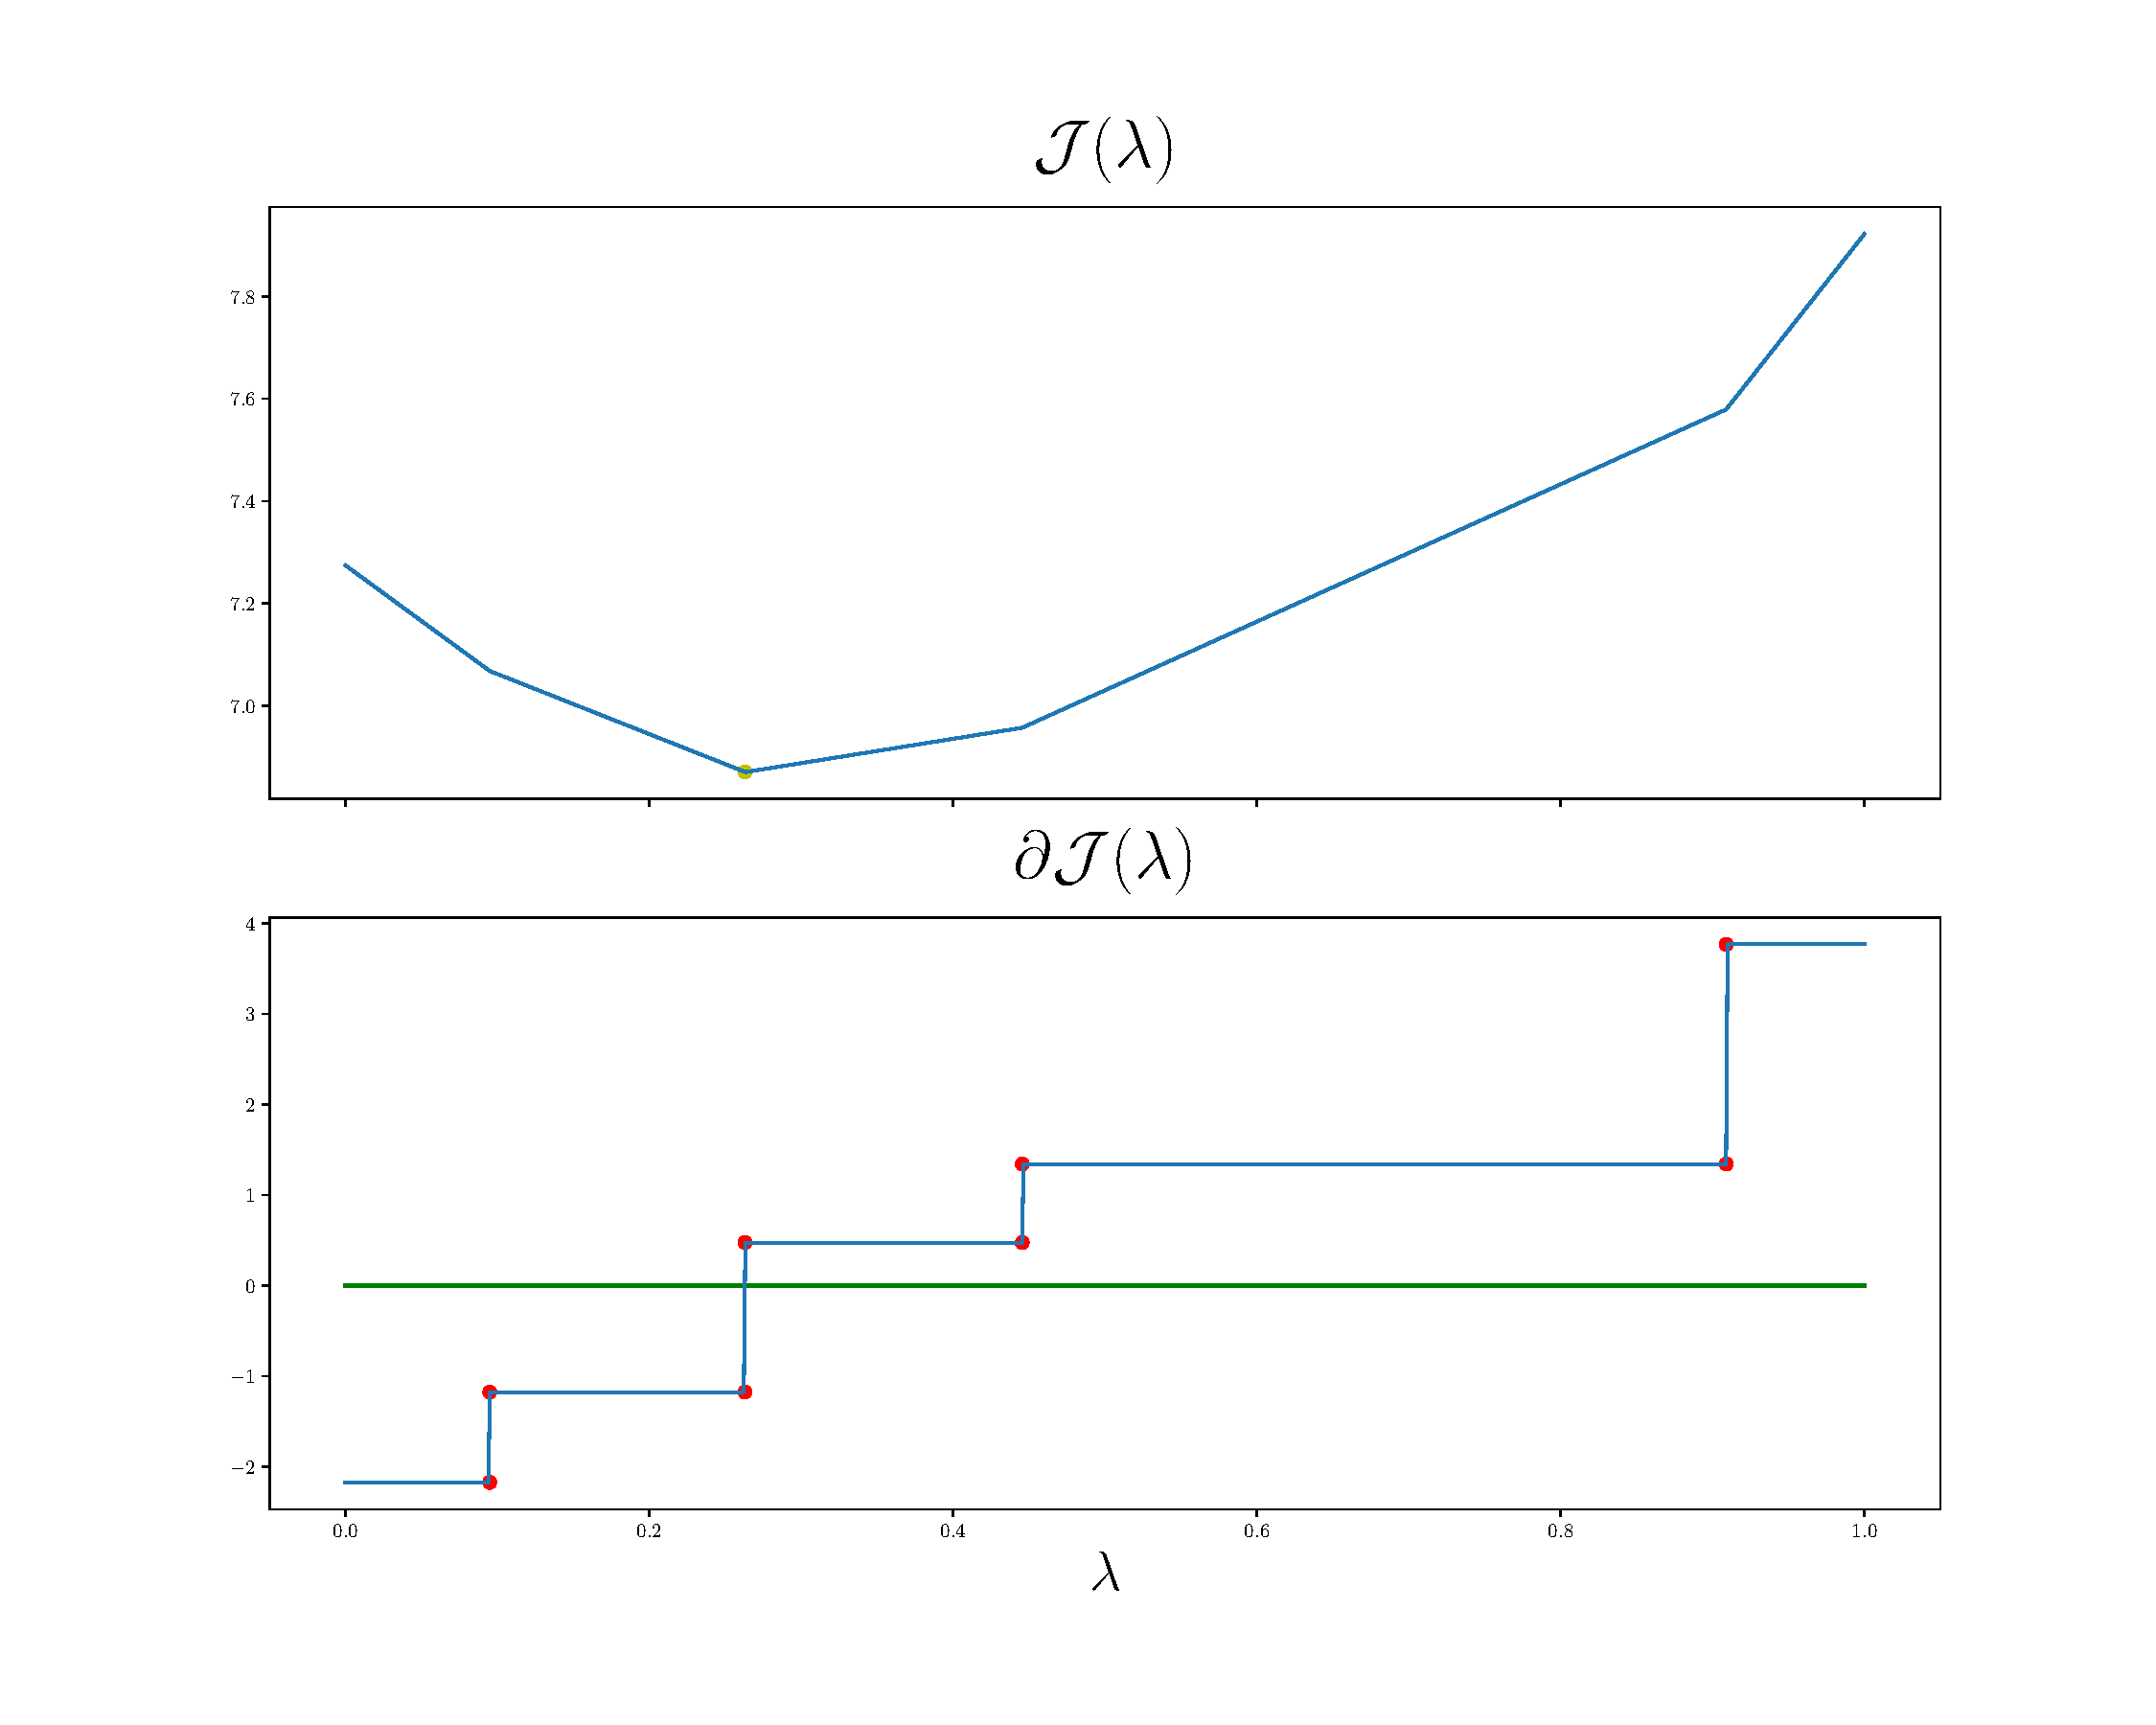
\includegraphics[width=.6\textwidth]{Chapter4/NeuroCom2021/ejemplo2_hinge.pdf}
% %             \label{fig:sq_error}
% %         \end{figure}      

% % \end{frame}


% \begin{frame}
%       \frametitle{Combinación Convexa con Error Hinge Cuadrático}


%       \begin{proposition}[$\lambda^*$ óptimo para el problema con error hinge cuadrático]\nonumber%\label{prop:hinge_neurocom2020}
%             \begin{itemize}
%                   \item $\lambda^*=0$ es óptimo si y solo si: $-\sum_{i:\; 0 > c_{(i)}, 0 < \lambda_{(i)}} {2 c_i d_i} - \sum_{i:\; 0 < c_{(i)}, 0 > \lambda_{(i)}} {2 c_i d_i}  \leq 0 $
%                   \item $\lambda^* \in (0,1)$ es óptimo si y solo si $0 < \lambda^* = \widehat{\lambda}_{(k)} < 1$ para algún $k=1, \dotsc, \npertask$, donde
%                   \begin{myequation}\nonumber%\label{eq:sol_hinge_2}
%                         \widehat{\lambda}_{(k)} = - \frac{\sum_{i:\; \lambda_{(k+1)} \geq \lambda_{(i)}} \mymax{0, c_{(i)}} d_{(i)} + \sum_{i:\; \lambda_{(k)} \leq \lambda_{(i)}} \mymin{0, c_{(i)}} d_{(i)}}{\sum_{i:\; \lambda_{(k+1)} \geq \lambda_{(i)}} \mymax{0, c_{(i)}}^2 + \sum_{i:\; \lambda_{(k)} \leq \lambda_{(i)}} \mymin{0, c_{(i)}}^2} ,
%                   \end{myequation}
%                   y además $\lambda_{(k)} \leq \widehat{\lambda}_k \leq  \lambda_{(k+1)}$
%                   \item $\lambda^*=1$ es óptimo en otro caso
%             \end{itemize}
%         \end{proposition}

%       % \begin{proposition}[Optimal $\lambda^*$ with Squared Hinge Loss]\label{prop:sqhinge_neurocom2020}
%       %       In~\eqref{eq:opt_hinge_l2},
%       %       $\lambda^*=0$ is optimal iff 
%       %       \begin{myequation}\nonumber
%       %           -\sum_{\substack{i:\; 0 > c_{(i)},\\ \;\; 0 < \lambda_{(i)}}} {2 c_i d_i} - \sum_{\substack{i:\; 0 < c_{(i)},\\ \;\; 0 > \lambda_{(i)}}} {2 c_i d_i}  \leq 0 .
%       %          \end{myequation}
%       %       If this condition does not hold, 
%       %       consider the sorted list of elbows $\lambda_{(1)}, \ldots, \lambda_{(\npertask)}$; then, for each interval between elbows $(\lambda_{(k)}, \lambda_{(k+1)})$, we define the value $\widehat{\lambda}_k$ for $k=1, \ldots,  \npertask-1$ as %
%       %   \begin{myequation}\label{eq:sol_hinge_2}
%       %       \widehat{\lambda}_{(k)} = - \frac{\sum_{i:\; \lambda_{(k+1)} \geq \lambda_{(i)}} \mymax{0, c_{(i)}} d_{(i)} + \sum_{i:\; \lambda_{(k)} \leq \lambda_{(i)}} \mymin{0, c_{(i)}} d_{(i)}}{\sum_{i:\; \lambda_{(k+1)} \geq \lambda_{(i)}} \mymax{0, c_{(i)}}^2 + \sum_{i:\; \lambda_{(k)} \leq \lambda_{(i)}} \mymin{0, c_{(i)}}^2} .
%       %   \end{myequation}
%       %   %
%       %   If $\widehat{\lambda}_k$ satisfies that $\lambda_{(k)} \leq \widehat{\lambda}_k \leq  \lambda_{(k+1)}$ and $0 \leq \widehat{\lambda}_{(k)} \leq 1$ for some $k=1, \ldots, \npertask$ then $\lambda^* = \widehat{\lambda}_k$ is optimal.
%       %   Finally, if none of the previous conditions holds, \eqref{eq:opt_hinge_l2} has a minimum at $\lambda^* = 1$.
%       %   \end{proposition}
% \end{frame}

% \begin{frame}

%       \begin{figure}[t!]
%             \centering
%             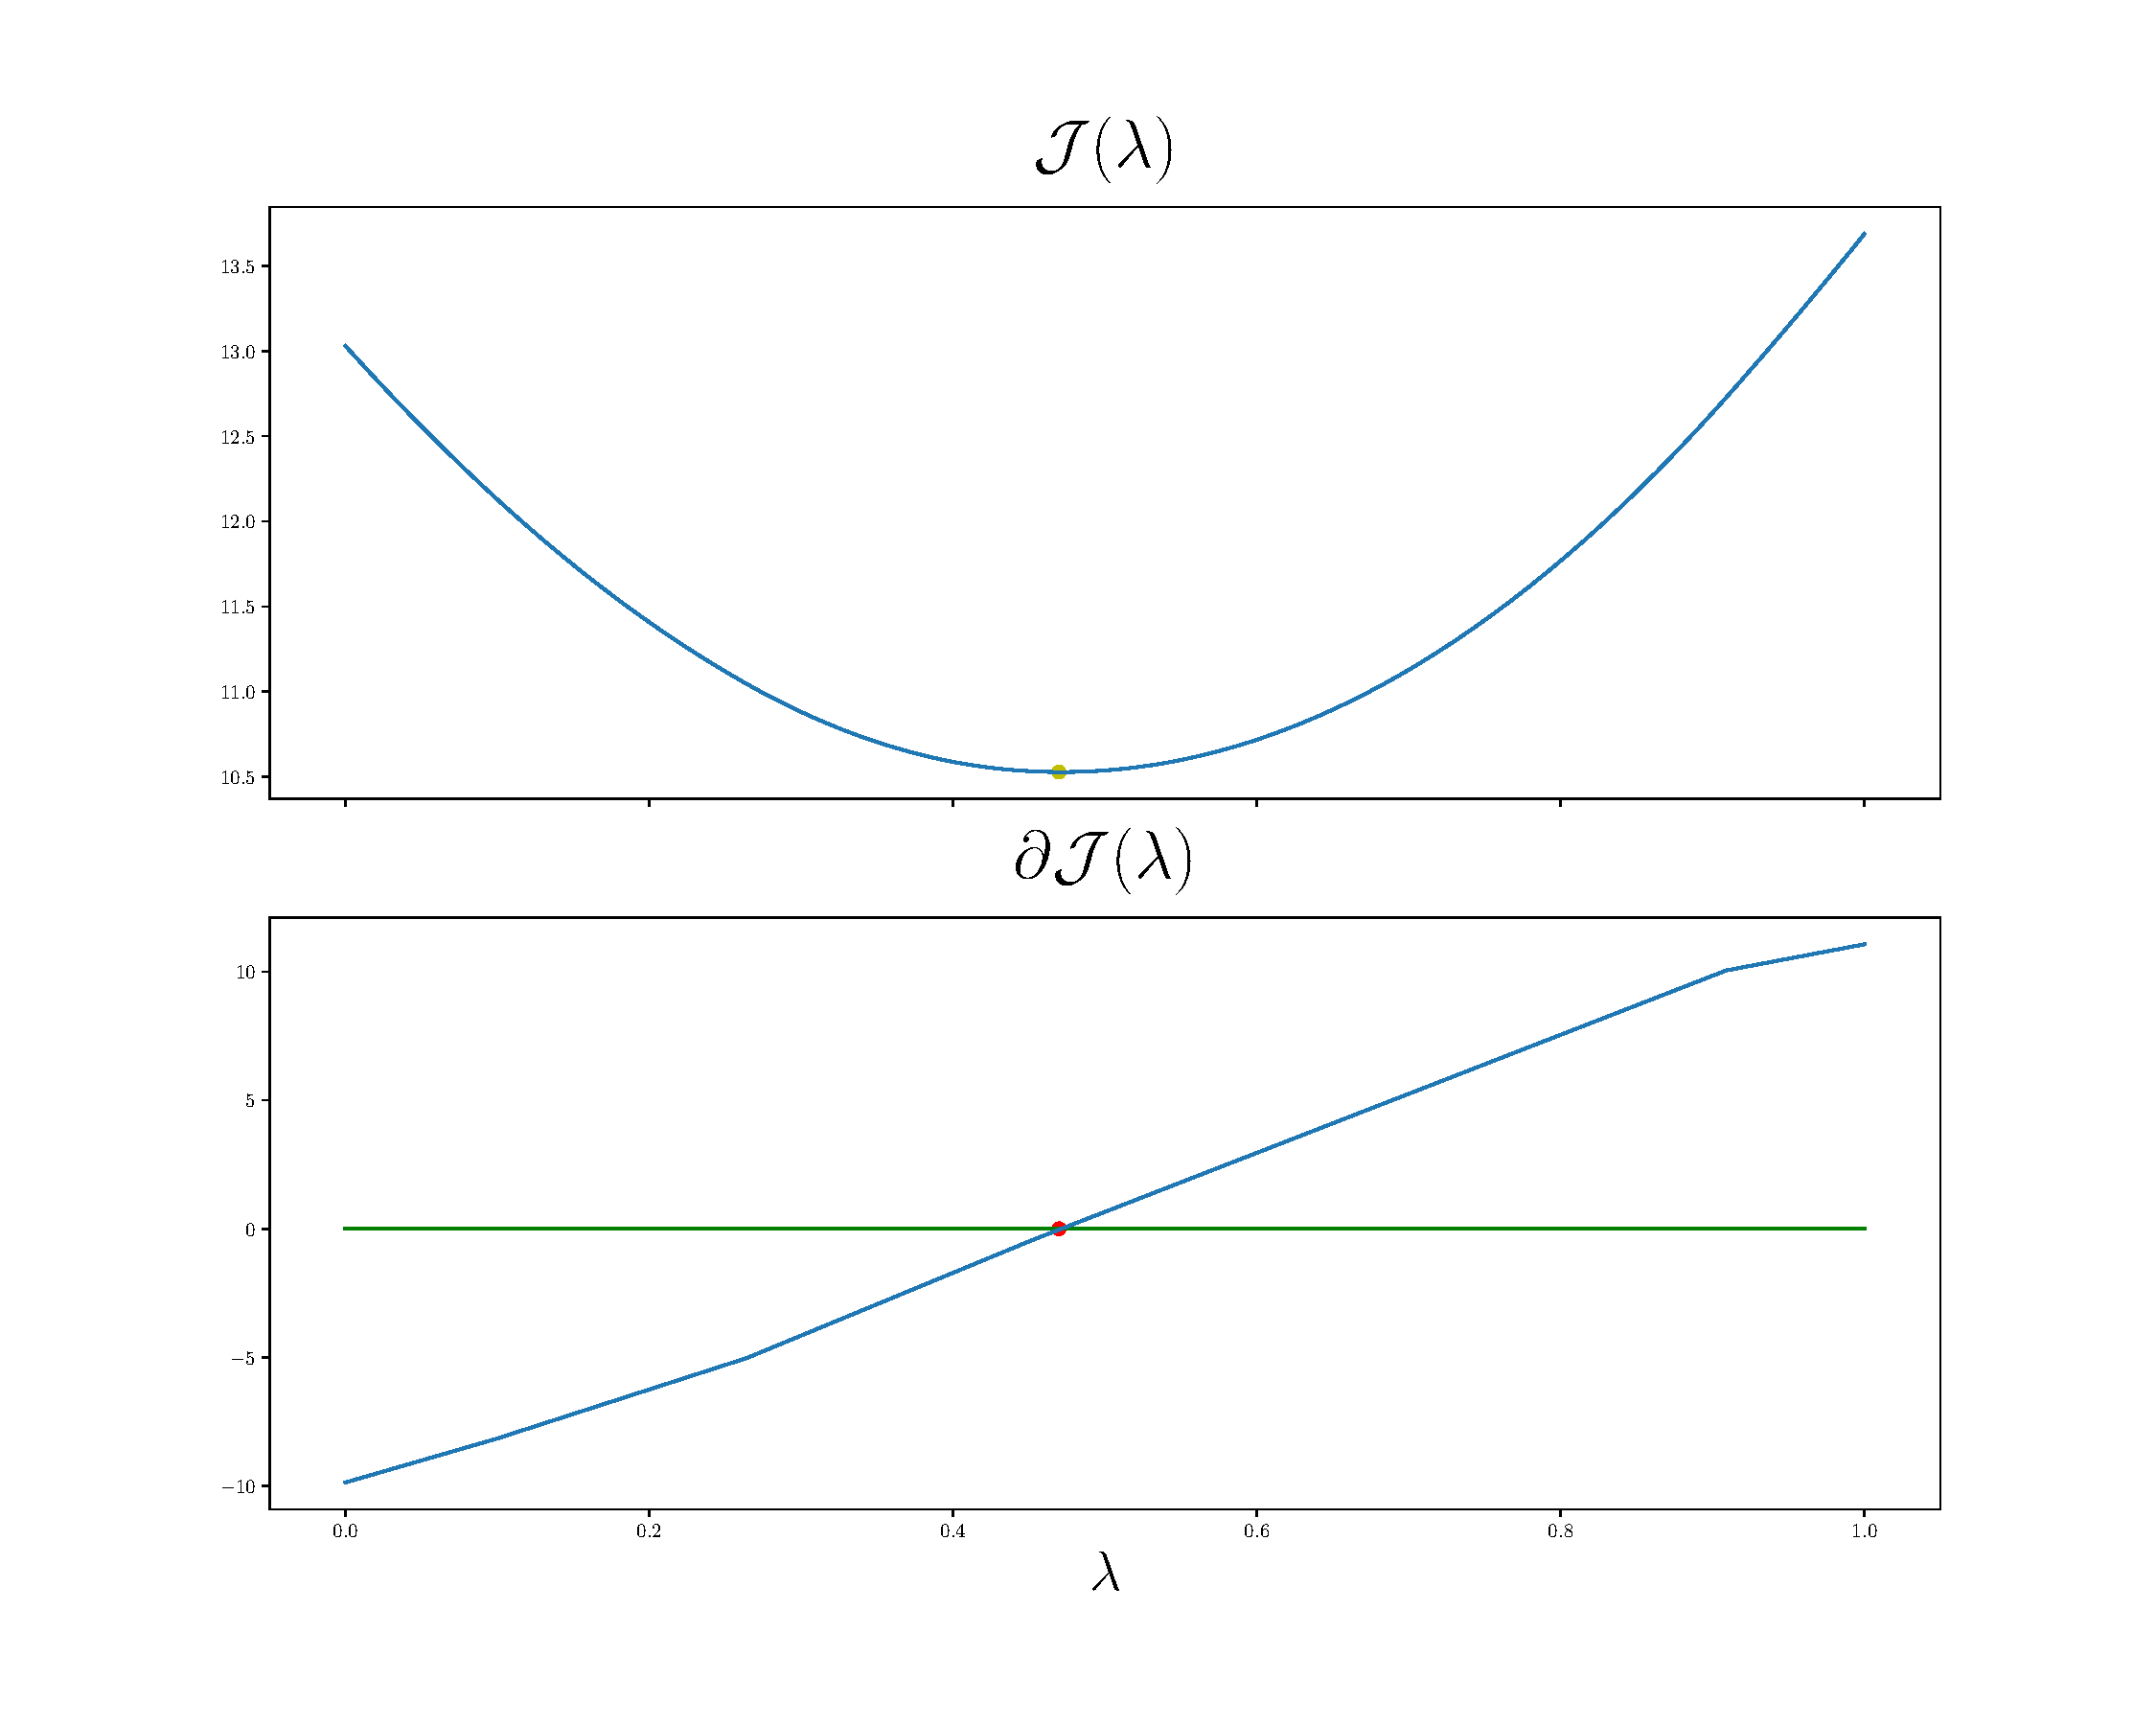
\includegraphics[width=.6\textwidth]{Chapter4/NeuroCom2021/ejemplo2_sqhinge.pdf}
%             \label{fig:sq_error}
%         \end{figure}      

% \end{frame}


% \begin{frame}
%       \frametitle{Experimentos}

      
%       \scalebox{.7}{
%       \begin{tabular}{l*{2}{c@{ }l}*{4}{r@{$\pm$}l@{ }l } }
%       \toprule
%       & \fheadmulti{2}{\fdata{maj.}} & \fheadmulti{2}{\fdata{ten.}} & \fheadmulti{3}{\fdata{boston}} & \fheadmulti{3}{\fdata{california}} &  \fheadmulti{3}{\fdata{abalone}} & \fheadmulti{3}{\fdata{crime}}\\
%       \midrule
%       & \fheadmulti{16}{MAE} \\
%       \midrule
%       \fmod{ITL-L1}            &  {5.087} &   (6) &  {5.743} &   (3) &  {2.341} & {0.229} &   \fmaxn{(1)} &  {36883.582} & {418.435} &   (2) &  {1.481} & {0.051} &   (3) &  {0.078} & {0.001} &   (2) \\
%       \fmod{CTL-L1}            &  {5.175} &   (7) &  {5.891} &   (5) &  \fmaxn{2.192} & \fmaxn{0.244} &   \fmaxn{(1)} &  {41754.337} & {270.908} &   (6) &  {1.482} & {0.050} &   (3) &  {0.078} & {0.001} &   (2) \\
%       \fmod{CMB-L1} &  \fmaxn{5.047} &   (5) &  \fmaxn{5.340} &  \fmaxn{(1)} &  {2.239} & {0.255} &   \fmaxn{(1)} &  {36880.238} & {420.417} &   \fmaxn{(1)} &  {1.470} & {0.052} &   (2) &  {0.077} & {0.002} &   (2) \\
%       \fmod{MTL-L1}     &  {5.050} &   (5) &  {5.535} &   (2) &  {2.206} & {0.292} &   \fmaxn{(1)} &  \fmaxn{36711.383} & \fmaxn{343.333} &  \fmaxn{(1)} &  \fmaxn{1.454} & \fmaxn{0.048} &  \fmaxn{(1)} &  \fmaxn{0.074} & \fmaxn{0.002} &  \fmaxn{(1)} \\
%       \midrule
%       \fmod{ITL-L2}            &  {4.952} &   (3) &  \fmaxn{5.629} &   (3) &  {2.356} & {0.300} &   \fmaxn{(1)} &  {37374.618} & {433.511} &   (5) &  {1.498} & {0.054} &   (4) &  {0.079} & {0.002} &   (2) \\
%       \fmod{CTL-L2}            &  {5.193} &   (7) &  {6.107} &   (8) &  \fmaxn{2.083} & \fmaxn{0.136} &   \fmaxn{(1)} &  {42335.612} & {163.773} &   (8) &  {1.503} & {0.047} &   (5) &  {0.080} & {0.002} &   (2) \\
%       \fmod{CMB-L2} &  {4.869} &   (3) &  {5.963} &   (6) &  {2.089} & {0.128} &   \fmaxn{(1)} &  {37374.618} & {433.511} &   (4) &  {1.494} & {0.050} &   (4) &  {0.077} & {0.003} &   (2) \\
%       \fmod{MTL-L2}     &  \fmaxn{4.854} &   (2) &  {5.784} &   (4) &  {2.089} & {0.134} &   \fmaxn{(1)} &  \fmaxn{37202.603} & \fmaxn{419.166} &   (3) &  \fmaxn{1.482} & \fmaxn{0.049} &   (3) &  \fmaxn{0.077} & \fmaxn{0.002} &   (2) \\
%       \midrule
%       \fmod{ITL-LS}            &  {4.937} &   (3) &  {5.649} &   (3) &  {2.204} & {0.116} &   \fmaxn{(1)} &  {37348.347} & {441.240} &   (4) &  {1.496} & {0.051} &   (4) &  {0.079} & {0.002} &   (2) \\
%       \fmod{CTL-LS}            &  {5.193} &   (7) &  {6.005} &   (7) &  \fmaxn{2.072} & \fmaxn{0.143} &  \fmaxn{(1)} &  {42259.492} & {146.825} &   (7) &  {1.502} & {0.052} &   (5) &  {0.079} & {0.002} &   (2) \\
%       \fmod{CMB-LS} &  {4.977} &   (4) &  \fmaxn{5.593} &   (3) &  {2.081} & {0.146} &   \fmaxn{(1)} &  {37339.179} & {430.288} &   (4) &  {1.486} & {0.049} &   (4) &  {0.079} & {0.002} &   (2) \\
%       \fmod{MTL-LS}     &  \fmaxn{4.824} &  \fmaxn{(1)} &  {5.754} &   (4) &  {2.077} & {0.152} &   \fmaxn{(1)} &  \fmaxn{37231.043} & \fmaxn{420.992} &   (4) &  \fmaxn{1.478} & \fmaxn{0.050} &   (3) &  \fmaxn{0.076} & \fmaxn{0.002} &   (2) \\
%       % \midrule
%       % & \fheadmulti{16}{R2} \\
%       % \midrule
%       % \fmod{ITL-L1}            &  {0.845} &   (6) &  {0.901} &   (7) &  {0.821} & {0.041} &   (2) &  {0.699} & {0.009} &   (7) &  {0.543} & {0.022} &   (8) &  {0.732} & {0.021} &   (3) \\
%       % \fmod{CTL-L1}            &  {0.837} &   (9) &  {0.901} &   (6) &  {0.854} & {0.036} &   \fmaxn{(1)} &  {0.639} & {0.006} &  (10) &  {0.559} & {0.014} &   (6) &  {0.740} & {0.027} &   (3) \\
%       % \fmod{CMB-L1} &  {0.844} &   (6) &  {0.905} &   (4) &  {0.845} & {0.053} &   \fmaxn{(1)} &  {0.699} & {0.009} &   (6) &  {0.555} & {0.018} &   (7) &  {0.741} & {0.029} &   (3) \\
%       % \fmod{MTL-L1}     &  \fmaxn{0.846} &   (4) &  \fmaxn{0.908} &   (2) &  \fmaxn{0.858} & \fmaxn{0.057} &   \fmaxn{(1)} &  \fmaxn{0.703} & \fmaxn{0.007} &   (6) &  \fmaxn{0.568} & \fmaxn{0.012} &   (5) &  \fmaxn{0.760} & \fmaxn{0.024} &   (2) \\
%       % \midrule
%       % \fmod{ITL-L2}            &  {0.846} &   (5) &  {0.906} &   (3) &  {0.836} & {0.045} &   (2) &  {0.707} & {0.009} &   (5) &  {0.565} & {0.025} &   (6) &  {0.743} & {0.017} &   (3) \\
%       % \fmod{CTL-L2}            &  {0.840} &   (8) &  {0.901} &   (8) &  \fmaxn{0.889} & \fmaxn{0.017} &   \fmaxn{(1)} &  {0.645} & {0.005} &   (9) &  {0.574} & {0.013} &   (4) &  {0.744} & {0.028} &   (3) \\
%       % \fmod{CMB-L2} &  {0.850} &   (3) &  {0.900} &   (9) &  {0.885} & {0.013} &   \fmaxn{(1)} &  {0.707} & {0.009} &   (4) &  {0.571} & {0.018} &   (4) &  {0.755} & {0.024} &   (3) \\
%       % \fmod{MTL-L2}     &  \fmaxn{0.863} &   (2) &  \fmaxn{0.908} &   \fmaxn{(1)} &  {0.888} & {0.015} &   \fmaxn{(1)} &  \fmaxn{0.709} & \fmaxn{0.008} &  \fmaxn{(1)} &  \fmaxn{0.580} & \fmaxn{0.014} &   (3) &  \fmaxn{0.762} & \fmaxn{0.028} &   \fmaxn{(1)} \\
%       % \midrule
%       % \fmod{ITL-LS}            &  {0.849} &   (3) &  {0.907} &   (3) &  {0.856} & {0.008} &   \fmaxn{(1)} &  {0.707} & {0.009} &   (3) &  {0.573} & {0.015} &   (4) &  {0.743} & {0.022} &   (3) \\
%       % \fmod{CTL-LS}            &  {0.838} &   (9) &  {0.904} &   (5) &  \fmaxn{0.894} & \fmaxn{0.015} &  \fmaxn{(1)} &  {0.646} & {0.005} &   (8) &  {0.576} & {0.016} &   (4) &  {0.746} & {0.032} &   (3) \\
%       % \fmod{CMB-LS} &  {0.843} &   (7) &  {0.907} &   (2) &  {0.886} & {0.024} &   \fmaxn{(1)} &  {0.707} & {0.009} &   (2) &  {0.581} & {0.012} &   (2) &  {0.746} & {0.021} &   (3) \\
%       % \fmod{MTL-LS}     &  \fmaxn{0.863} &  \fmaxn{(1)} &  \fmaxn{0.910} &  \fmaxn{(1)} &  {0.890} & {0.016} &   \fmaxn{(1)} &  \fmaxn{0.709} & \fmaxn{0.008} &   (2) &  \fmaxn{0.581} & \fmaxn{0.015} &  \fmaxn{(1)} &  \fmaxn{0.763} & \fmaxn{0.028} &  \fmaxn{(1)} \\
%       \bottomrule
%       \end{tabular}}

% \end{frame}


\begin{frame}
      \frametitle{Experimentos: Modelos}
  
  \begin{itemize}
      \item \textbf{Common Task Learning LX-SVM (\fmod{CTL-LX})}: Un único modelo LX-SVM que es común para todas las tareas
      \item \textbf{Independent Task Learning LX-SVM (\fmod{ITL-LX})}: Un modelo LX-SVM independiente para cada tarea
      \item \textbf{Direct Convex Combination of LX-SVMs (\fmod{CMB-LX})}: Una combinación convexa de los mejores \fmod{CTL-LX} y \fmod{ITL-LX}
      \item \textbf{Convex Multi-Task Learning LX-SVM (\fmod{MTL-LX})}: Un modelo multitarea con la formulación convexa basado en la LX-SVM
  
  \end{itemize}   
  
  \end{frame}
  
  \begin{frame}
      \frametitle{Experimentos: Problemas}
  
      \begin{table}
          \centering
          \scalebox{.7}{
          \begin{tabular}{l*{7}{S[table-format=5]}}
          \toprule
          \fhead{Problema} & \fhead{Tamaño} & \fhead{Dimensión} & \fhead{Nº tareas} & \fhead{Tam. tarea medio} & \fhead{Tam. tarea mín.} & \fhead{Tam. tarea máx.}\\
          \midrule
      %      & \multicolumn{6}{c}{\fhead{Regresión}} \\
      %     \midrule
          \fdata{majorca} & 15330 & 765 & 14 & 1095 & 1095 & 1095 \\ 
          \fdata{tenerife} & 15330 & 765 & 14 & 1095 & 1095 & 1095 \\
          \fdata{california} & 19269 & 9 & 5 & 3853 & 5 & 8468\\
          \fdata{boston} & 506 & 12 & 2 & 253 & 35 & 471 \\
          \fdata{abalone} & 4177 & 8 & 3 & 1392 & 1307 & 1527 \\
          \fdata{crime} & 1195 & 127 & 9 & 132 & 60  & 278 \\
          \midrule
      %     \multicolumn{7}{c}{\fhead{Regresión}} \\
      %     \midrule
          \fdata{binding} & 32302 & 184 & 47 & 687 & 59 & 3089 \\ 
          \fdata{landmine} & 14820 & 10 & 28 & 511 & 445 & 690 \\
          \fdata{adult\_(G)} & 48842 & 106 & 2 & 24421 & 16192 & 32650 \\
          \fdata{adult\_(R)} & 48842 & 103 & 5 & 9768 & 406 & 41762 \\
          \fdata{adult\_(G, R)} & 48842 & 101 & 10 & 4884 & 155 & 28735 \\
          \fdata{compas\_(G)} & 3987 & 11 & 2 & 1993 & 840 & 3147 \\
          \fdata{compas\_(R)} & 3987 & 9 & 4 & 997 & 255 & 1918 \\
          \fdata{compas\_(G, R)} & 3987 & 7 & 8 & 498 & 50 & 1525 \\
          \bottomrule
         \end{tabular}}
      \end{table}
  
  \end{frame}
  
  \begin{frame}
      \frametitle{Experimentos: Procedimiento}
  
      \begin{itemize}
          \item Para \fdata{majorca} y \fdata{tenerife}, usamos los datos de 2013, 2014 and 2015 como conjuntos de entrenamiento, validación y test, respectivamente
          \item Para el resto, usamos una CV anidada con 3 particiones externas e internas estratificadas por tareas
          \item Los hiperparámetros se eligen con una búsqueda en rejilla con las particiones de entrenamiento y validación
          \item Obtenemos $3$ scores de test para cada modelo en cada problema
      \end{itemize}
  
  \end{frame}
  
  \begin{frame}
      \frametitle{Experimentos: Hiperparámetros}
  
      \begin{itemize}
          \item Por limitaciones computacionales nos restringimos a la búsqueda de tres hiperparámetros para la búsqueda en rejilla
          \item Las anchuras de kernel para los modelos MTL se extraen de los modelos CTL e ITL
      \end{itemize}
  
      \begin{table}[t]
          \centering
          \scalebox{.7}{
           \begin{tabular}{*{9}{c}}
           \toprule
           \fhead{} & \fhead{Rejilla} & \fhead{\fmod{CTL-L1,2}} & \fhead{\fmod{ITL-L1,2}} & \fhead{\fmod{MTL-L1,2}}  & \fhead{\fmod{CTL-LS}} & \fhead{\fmod{ITL-LS}} & \fhead{\fmod{MTL-LS}}   \\
           \midrule
            $C$ &  \scalebox{.9}{$\set{4^k: -2 \leq k \leq 6}$} & CV & CV & CV & CV & CV & CV  \\ 
            $\epsilon$ & \scalebox{.9}{$\set{\frac{\sigma}{4^k}: 1 \leq k \leq 6}$} & CV & CV & CV & - & - & - \\
            $\gamma_c$ & \scalebox{.9}{$\set{\frac{4^k}{d}: -2 \leq k \leq 3}$} & CV & - & \fmod{CTL-L1,2} & CV & - & \fmod{CTL-LS} \\
            $\gamma_s^r$ & \scalebox{.9}{$\set{\frac{4^k}{d}: -2 \leq k \leq 3}$} & - & CV & \fmod{ITL-L1,2} & - & CV & \fmod{ITL-LS}\\
            $\lambda$ & \scalebox{.9}{$\set{0.1 k : 0 \leq k \leq 10}$} & - & - & CV & - & - & CV \\
            \bottomrule
           \end{tabular}
           }
      \end{table}
  
  \end{frame}
  
  \begin{frame}{Experimentos: Resultados de Regresión (MAE)}
  
      \begin{table}[t]
          % \caption{Test MAE for the models selected using the MAE for hyperparametrization. The best model is shown in bold in each block of models. The global ranking given by the pairwise Wilcoxon test is also given.}
          \label{tab:error_models_reg_mae_mae}
          \centering
          \scalebox{.7}{
          \begin{tabular}{l*{2}{S[table-format=1.3]@{ }l}*{4}{S[table-format=1.3]@{$\pm$}S[table-format=1.3]@{ }l } }
          \toprule
          & \fheadmulti{2}{\fdata{maj.}} & \fheadmulti{2}{\fdata{ten.}} & \fheadmulti{3}{\fdata{boston}} & \fheadmulti{3}{\fdata{california}} &  \fheadmulti{3}{\fdata{abalone}} & \fheadmulti{3}{\fdata{crime}}\\
          \midrule
          \fmod{ITL-L1}            &  {5.087} &   (6) &  {5.743} &   (3) &  {2.341} & {0.229} &   \fmaxn{(1)} &  {36883.582} & {418.435} &   (2) &  {1.481} & {0.051} &   (3) &  {0.078} & {0.001} &   (2) \\
          \fmod{CTL-L1}            &  {5.175} &   (7) &  {5.891} &   (5) &  \fmaxn{2.192} & \fmaxn{0.244} &   \fmaxn{(1)} &  {41754.337} & {270.908} &   (6) &  {1.482} & {0.050} &   (3) &  {0.078} & {0.001} &   (2) \\
          \fmod{CMB-L1} &  \fmaxn{5.047} &   (5) &  \fmaxn{5.340} &  \fmaxn{(1)} &  {2.239} & {0.255} &   \fmaxn{(1)} &  {36880.238} & {420.417} &   \fmaxn{(1)} &  {1.470} & {0.052} &   (2) &  {0.077} & {0.002} &   (2) \\
          \fmod{MTL-L1}     &  {5.050} &   (5) &  {5.535} &   (2) &  {2.206} & {0.292} &   \fmaxn{(1)} &  \fmaxn{36711.383} & \fmaxn{343.333} &  \fmaxn{(1)} &  \fmaxn{1.454} & \fmaxn{0.048} &  \fmaxn{(1)} &  \fmaxn{0.074} & \fmaxn{0.002} &  \fmaxn{(1)} \\
          \midrule
          \fmod{ITL-L2}            &  {4.952} &   (3) &  \fmaxn{5.629} &   (3) &  {2.356} & {0.300} &   \fmaxn{(1)} &  {37374.618} & {433.511} &   (5) &  {1.498} & {0.054} &   (4) &  {0.079} & {0.002} &   (2) \\
          \fmod{CTL-L2}            &  {5.193} &   (7) &  {6.107} &   (8) &  \fmaxn{2.083} & \fmaxn{0.136} &   \fmaxn{(1)} &  {42335.612} & {163.773} &   (8) &  {1.503} & {0.047} &   (5) &  {0.080} & {0.002} &   (2) \\
          \fmod{CMB-L2} &  {4.869} &   (3) &  {5.963} &   (6) &  {2.089} & {0.128} &   \fmaxn{(1)} &  {37374.618} & {433.511} &   (4) &  {1.494} & {0.050} &   (4) &  {0.077} & {0.003} &   (2) \\
          \fmod{MTL-L2}     &  \fmaxn{4.854} &   (2) &  {5.784} &   (4) &  {2.089} & {0.134} &   \fmaxn{(1)} &  \fmaxn{37202.603} & \fmaxn{419.166} &   (3) &  \fmaxn{1.482} & \fmaxn{0.049} &   (3) &  \fmaxn{0.077} & \fmaxn{0.002} &   (2) \\
          \midrule
          \fmod{ITL-LS}            &  {4.937} &   (3) &  {5.649} &   (3) &  {2.204} & {0.116} &   \fmaxn{(1)} &  {37348.347} & {441.240} &   (4) &  {1.496} & {0.051} &   (4) &  {0.079} & {0.002} &   (2) \\
          \fmod{CTL-LS}            &  {5.193} &   (7) &  {6.005} &   (7) &  \fmaxn{2.072} & \fmaxn{0.143} &  \fmaxn{(1)} &  {42259.492} & {146.825} &   (7) &  {1.502} & {0.052} &   (5) &  {0.079} & {0.002} &   (2) \\
          \fmod{CMB-LS} &  {4.977} &   (4) &  \fmaxn{5.593} &   (3) &  {2.081} & {0.146} &   \fmaxn{(1)} &  {37339.179} & {430.288} &   (4) &  {1.486} & {0.049} &   (4) &  {0.079} & {0.002} &   (2) \\
          \fmod{MTL-LS}     &  \fmaxn{4.824} &  \fmaxn{(1)} &  {5.754} &   (4) &  {2.077} & {0.152} &   \fmaxn{(1)} &  \fmaxn{37231.043} & \fmaxn{420.992} &   (4) &  \fmaxn{1.478} & \fmaxn{0.050} &   (3) &  \fmaxn{0.076} & \fmaxn{0.002} &   (2) \\
          \bottomrule
          \end{tabular}}
        \end{table}
  
  \end{frame}
  
  
%   \begin{frame}{Experimentos: Resultados de Regresión (MSE)}
  
%       \begin{table}[t]
%           \label{tab:error_models_reg_mae_r2}
%           \centering
%           \scalebox{.7}{
%           \begin{tabular}{l*{2}{S[table-format=1.3]@{ }l}*{4}{S[table-format=1.3]@{$\pm$}S[table-format=1.3]@{ }l } }
%           \toprule
%               & \fheadmulti{2}{\fdata{maj.}} & \fheadmulti{2}{\fdata{ten.}} & \fheadmulti{3}{\fdata{boston}} & \fheadmulti{3}{\fdata{california}} &  \fheadmulti{3}{\fdata{abalone}} & \fheadmulti{3}{\fdata{crime}}\\
%               \midrule
%           \fmod{ITL-L1}            &  {0.845} &   (6) &  {0.901} &   (7) &  {0.821} & {0.041} &   (2) &  {0.699} & {0.009} &   (7) &  {0.543} & {0.022} &   (8) &  {0.732} & {0.021} &   (3) \\
%           \fmod{CTL-L1}            &  {0.837} &   (9) &  {0.901} &   (6) &  {0.854} & {0.036} &   \fmaxn{(1)} &  {0.639} & {0.006} &  (10) &  {0.559} & {0.014} &   (6) &  {0.740} & {0.027} &   (3) \\
%           \fmod{CMB-L1} &  {0.844} &   (6) &  {0.905} &   (4) &  {0.845} & {0.053} &   \fmaxn{(1)} &  {0.699} & {0.009} &   (6) &  {0.555} & {0.018} &   (7) &  {0.741} & {0.029} &   (3) \\
%           \fmod{MTL-L1}     &  \fmaxn{0.846} &   (4) &  \fmaxn{0.908} &   (2) &  \fmaxn{0.858} & \fmaxn{0.057} &   \fmaxn{(1)} &  \fmaxn{0.703} & \fmaxn{0.007} &   (6) &  \fmaxn{0.568} & \fmaxn{0.012} &   (5) &  \fmaxn{0.760} & \fmaxn{0.024} &   (2) \\
%           \midrule
%           \fmod{ITL-L2}            &  {0.846} &   (5) &  {0.906} &   (3) &  {0.836} & {0.045} &   (2) &  {0.707} & {0.009} &   (5) &  {0.565} & {0.025} &   (6) &  {0.743} & {0.017} &   (3) \\
%           \fmod{CTL-L2}            &  {0.840} &   (8) &  {0.901} &   (8) &  \fmaxn{0.889} & \fmaxn{0.017} &   \fmaxn{(1)} &  {0.645} & {0.005} &   (9) &  {0.574} & {0.013} &   (4) &  {0.744} & {0.028} &   (3) \\
%           \fmod{CMB-L2} &  {0.850} &   (3) &  {0.900} &   (9) &  {0.885} & {0.013} &   \fmaxn{(1)} &  {0.707} & {0.009} &   (4) &  {0.571} & {0.018} &   (4) &  {0.755} & {0.024} &   (3) \\
%           \fmod{MTL-L2}     &  \fmaxn{0.863} &   (2) &  \fmaxn{0.908} &   \fmaxn{(1)} &  {0.888} & {0.015} &   \fmaxn{(1)} &  \fmaxn{0.709} & \fmaxn{0.008} &  \fmaxn{(1)} &  \fmaxn{0.580} & \fmaxn{0.014} &   (3) &  \fmaxn{0.762} & \fmaxn{0.028} &   \fmaxn{(1)} \\
%           \midrule
%           \fmod{ITL-LS}            &  {0.849} &   (3) &  {0.907} &   (3) &  {0.856} & {0.008} &   \fmaxn{(1)} &  {0.707} & {0.009} &   (3) &  {0.573} & {0.015} &   (4) &  {0.743} & {0.022} &   (3) \\
%           \fmod{CTL-LS}            &  {0.838} &   (9) &  {0.904} &   (5) &  \fmaxn{0.894} & \fmaxn{0.015} &  \fmaxn{(1)} &  {0.646} & {0.005} &   (8) &  {0.576} & {0.016} &   (4) &  {0.746} & {0.032} &   (3) \\
%           \fmod{CMB-LS} &  {0.843} &   (7) &  {0.907} &   (2) &  {0.886} & {0.024} &   \fmaxn{(1)} &  {0.707} & {0.009} &   (2) &  {0.581} & {0.012} &   (2) &  {0.746} & {0.021} &   (3) \\
%           \fmod{MTL-LS}     &  \fmaxn{0.863} &  \fmaxn{(1)} &  \fmaxn{0.910} &  \fmaxn{(1)} &  {0.890} & {0.016} &   \fmaxn{(1)} &  \fmaxn{0.709} & \fmaxn{0.008} &   (2) &  \fmaxn{0.581} & \fmaxn{0.015} &  \fmaxn{(1)} &  \fmaxn{0.763} & \fmaxn{0.028} &  \fmaxn{(1)} \\
%           \bottomrule
%          \end{tabular}}
%         \end{table}
  
%   \end{frame}
  
  
  
  \begin{frame}{Experimentos: Resultados de Clasificación (Score F1)}
  
      \begin{table}[t]
          \label{tab:error_models_class_f1}
          \centering
          \scalebox{.7}{
            \begin{tabular}{ l*{8}{S[table-format=1.3]} c c c}
              \toprule
              & \fhead{\fdata{comp\_(G)}} & \fhead{\fdata{comp\_(R)}} & \fhead{\fdata{comp\_(G,R)}} & \fhead{\fdata{ad\_(G)}} & \fhead{\fdata{ad\_(R)}} & \fhead{\fdata{ad\_(G,R)}} & \fhead{\fdata{landmine}} & \fhead{\fdata{binding}} & \fhead{mean} & \fhead{rank} & \fhead{Wil.}\\
              \midrule
              \fmod{ITL-L1}    &          0.625 &           \fmaxn{0.639} &                  0.630 &         \fmaxn{0.659} &          0.653 &                 0.657 &    0.231 &   0.867 & 0.620 &     10 & 2 \\
              \fmod{CTL-L1}    &          0.623 &           0.638 &                  0.638 &         0.657 &          0.650 &                 0.653 &    0.255 &   0.901 & 0.627 &      7 & 2 \\
              \fmod{CMB-L1} &          0.616 &           0.638 &                  0.638 &         0.658 &          0.650 &                 0.653 &    \fmaxn{0.270} &   0.901 & \fmaxn{0.628} &      6 & 2 \\
              \fmod{MTL-L1}    &          \fmaxn{0.627} &           0.636 &                  \fmaxn{0.640} &         \fmaxn{0.659} &          \fmaxn{0.655} &                 \fmaxn{0.659} &    0.242 &   \fmaxn{0.907} & \fmaxn{0.628} &      5 & 2 \\
              \midrule
              \fmod{ITL-L2}    &          0.636 &           0.623 &                  0.607 &         \fmaxn{0.668} &          \fmaxn{0.666} &                 \fmaxn{0.668} &    0.256 &   0.867 & 0.624 &      8 & 2 \\
              \fmod{CTL-L2}    &          \fmaxn{0.640} &           0.647 &                  \fmaxn{0.651} &         0.665 &          0.661 &                 0.659 &    \fmaxn{0.270} &   0.903 & 0.637 &      2 & 2 \\
              \fmod{CMB-L2} &          0.629 &           0.640 &                  0.645 &         0.666 &          0.662 &                 0.661 &    \fmaxn{0.270} &   0.903 & 0.634 &      3 & 2 \\
              \fmod{MTL-L2}    &          0.634 &           \fmaxn{0.651} &                  0.650 &         \fmaxn{0.668} &          \fmaxn{0.666} &                 \fmaxn{0.668} &    0.263 &   \fmaxn{0.909} & \fmaxn{0.639} &      1 & 1 \\
              \midrule
              \fmod{ITL-LS}    &          \fmaxn{0.631} &           0.622 &                  0.608 &         \fmaxn{0.659} &          \fmaxn{0.659} &                 \fmaxn{0.660} &    0.243 &   0.867 & 0.619 &     12 & 2 \\
              \fmod{CTL-LS}    &          0.628 &           \fmaxn{0.644} &                  \fmaxn{0.649} &         0.650 &          0.653 &                 0.647 &    0.230 &   0.853 & 0.619 &     11 & 2 \\
              \fmod{CMB-LS} &          0.630 &           0.635 &                  0.642 &         0.657 &          0.658 &                 0.654 &    0.238 &   0.873 & 0.623 &      9 & 2 \\
              \fmod{MTL-LS}    &          0.630 &           0.641 &                  0.648 &         \fmaxn{0.659} &          \fmaxn{0.659} &                 0.659 &    \fmaxn{0.257} &   \fmaxn{0.906} & \fmaxn{0.632} &      4 & 2 \\
              \bottomrule
            \end{tabular}}
        \end{table}
  
  \end{frame}
  
  
%   \begin{frame}{Experimentos: Resultados de Clasificación (Accuracy)}
  
%       \begin{table}[t]
%           \label{tab:error_models_class_acc}
%           \centering
%           \scalebox{.7}{
%           \begin{tabular}{ l*{8}{S[table-format=1.3]} c c c}
%           \toprule
%           & \fhead{\fdata{comp\_(G)}} & \fhead{\fdata{comp\_(R)}} & \fhead{\fdata{comp\_(G,R)}} & \fhead{\fdata{ad\_(G)}} & \fhead{\fdata{ad\_(R)}} & \fhead{\fdata{ad\_(G,R)}} & \fhead{\fdata{landmine}} & \fhead{\fdata{binding}} & \fhead{mean} & \fhead{rank}  & \fhead{Wil.}\\
%           \midrule
%           \fmod{ITL-L1}    &          0.750 &           0.749 &                  0.746 &         0.852 &          0.851 &                 \fmaxn{0.853} &    \fmaxn{0.941} &   0.790 & 0.817 &     11 & 3 \\
%           \fmod{CTL-L1}    &          \fmaxn{0.757} &           0.759 &                  \fmaxn{0.763} &         0.852 &          0.847 &                 0.849 &    0.938 &   0.850 & 0.827 &      6 & 1 \\
%           \fmod{CMB-L1} &          0.754 &           0.759 &                  \fmaxn{0.763} &         0.852 &          0.847 &                 0.849 &    0.935 &   0.850 & 0.826 &      7 & 2 \\
%           \fmod{MTL-L1}    &          0.753 &           \fmaxn{0.760} &                  \fmaxn{0.763} &         \fmaxn{0.853} &          \fmaxn{0.852} &                 \fmaxn{0.853} &    0.933 &   \fmaxn{0.861} & \fmaxn{0.829} &      5 & 1 \\
%           \midrule
%           \fmod{ITL-L2}    &          0.754 &           0.762 &                  0.751 &         \fmaxn{0.856} &          \fmaxn{0.855} &                 \fmaxn{0.856} &    \fmaxn{0.942} &   0.791 & 0.821 &      8 & 2 \\
%           \fmod{CTL-L2}    &          \fmaxn{0.762} &           0.765 &                  \fmaxn{0.767} &         0.854 &          0.853 &                 0.851 &    0.933 &   0.853 & 0.830 &      3 & 1 \\
%           \fmod{CMB-L2} &          0.757 &           0.764 &                  0.766 &         0.854 &          0.853 &                 0.853 &    0.934 &   0.853 & 0.829 &      4 & 1 \\
%           \fmod{MTL-L2}    &          0.753 &           \fmaxn{0.766} &                  0.766 &         \fmaxn{0.856} &          \fmaxn{0.855} &                 \fmaxn{0.856} &    0.933 &   \fmaxn{0.864} & \fmaxn{0.831} &      1 & 1 \\
%           \midrule
%           \fmod{ITL-LS}    &          0.754 &           0.761 &                  0.750 &         \fmaxn{0.851} &          \fmaxn{0.850} &                 \fmaxn{0.851} &    0.943 &   0.791 & 0.819 &      9 & 3 \\
%           \fmod{CTL-LS}    &          \fmaxn{0.757} &           \fmaxn{0.764} &                  0.766 &         0.845 &          0.847 &                 0.842 &    0.914 &   0.750 & 0.811 &     12 & 3 \\
%           \fmod{CMB-LS} &          0.754 &           \fmaxn{0.764} &                  0.765 &         0.849 &          \fmaxn{0.850} &                 0.848 &    0.925 &   0.793 & 0.818 &     10 & 3 \\
%           \fmod{MTL-LS}    &          \fmaxn{0.757} &           \fmaxn{0.764} &                  \fmaxn{0.767} &         \fmaxn{0.851} &          \fmaxn{0.850} &                 \fmaxn{0.851} &    \fmaxn{0.944} &   \fmaxn{0.858} & \fmaxn{0.830} &      2 & 1 \\
%           \bottomrule  
%         \end{tabular}}
%         \end{table}
  
%   \end{frame}

  


%%%%%%%%%%%%%%%%%%%%%%%%%%%%%%%%%%%%%%%%%%%%%%%%%%%%%%%%%%%%%%%%%%%%%%%%5
  \section{Formulación Convexa para Aprendizaje Multitarea: Redes Neuronales}


\begin{frame}
      \frametitle{Redes Neuronales MT}

      \begin{itemize}
            \item Los métodos de kernel ofrecen propiedades deseables como
            \begin{itemize}
                  \item convexidad
                  \item dualidad
                  \item truco del kernel
            \end{itemize}
            pero tienen una limitación computacional
            \item Las redes neuronales son mejores alternativas para grandes volúmenes de datos
            \item Existen arquitecturas neuronales específicas para algunos tipos de datos:
            \begin{itemize}
                  \item imágenes
                  \item texto
                  \item sonido
            \end{itemize}
            \item Proponemos una arquitectura MT para redes basada en la combinación convexa
      \end{itemize}

\end{frame}

%\subsection{Convex Multi-Task Learning with Neural Networks}
\begin{frame}
      \frametitle{Redes Neuronales MT: \emph{Hard Sharing}}

      \begin{itemize}
            \item La manera más común de adaptar las redes neuronales es el \emph{hard sharing}~\footfullcite{Caruana97}
            \begin{itemize}
                  \item Capas ocultas compartidas por todas las tareas
                  \item Capas de salida específicas para cada tarea
            \end{itemize}
            \item El modelo se puede expresar como:
            \begin{myequation}
                  \nonumber
                  %\label{eq:convexmtl_nn}
                  \begin{aligned}
                      h_r(\cdot) &=  g_r(\cdot; w_r, d_r, \Theta)
                     =  \lbrace \dotp{w_r}{f(\cdot; \Theta)} \rbrace + d_r
                  \end{aligned}
            \end{myequation}
            \begin{itemize}
                  \item $w_r, d_r$ son los parámetros de las capas de salida específicas
                  \item $\Theta$ son los parámetros de las capas ocultas compartidas
            \end{itemize}
            \item Se comparte la misma representación en todas las tareas 
      \end{itemize}

\end{frame}


\begin{frame}{Ejemplo de \emph{Hard Sharing} para dos tareas}

      \begin{figure}[t!]
    \centering
    \begin{tikzpicture}
 
        % Input Layer
        \foreach \i in {1,...,\inputnum}
        {
            \node[circle, 
                minimum size = 6mm,
                fill=orange!30] (Input-\i) at (0,-\i) {};
        }
         
        
        % Hidden Layer 1
        \foreach \i in {1,...,\hiddennumhs}
        {
            \node[circle, 
                minimum size = 6mm,
                fill=teal!50,
                yshift=(\hiddennumhs-\inputnum)*5 mm
            ] (Hidden1-\i) at (2.5,-\i) {};
        }
        
        % Hidden Layer 2
        \foreach \i in {1,...,\hiddennumhs}
        {
            \node[circle, 
                minimum size = 6mm,
                fill=teal!50,
                yshift=(\hiddennumhs-\inputnum)*5 mm
            ] (Hidden2-\i) at (5,-\i) {};
        }
         
        % Output Layer
        \foreach \i in {1,...,\outputnum}
        {
            \node[circle, 
                minimum size = 6mm,
                fill=purple!50,
                yshift=(\outputnum-\inputnum)*5 mm
            ] (Output-\i) at (7.5,-\i) {};
        }
         
        % Connect neurons In-Hidden
        \foreach \i in {1,...,\inputnum}
        {
            \foreach \j in {1,...,\hiddennumhs}
            {
                \draw[->, shorten >=1pt, red!80!black, densely dashdotted] (Input-\i) -- (Hidden1-\j);   
            }
        }

        % Connect neurons Hidden-Hidden
        \foreach \i in {1,...,\hiddennumhs}
        {
            \foreach \j in {1,...,\hiddennumhs}
            {
                \draw[->, shorten >=1pt, red!80!black, densely dashdotted] (Hidden1-\i) -- (Hidden2-\j);   
            }
        }
         
        % Connect neurons Hidden-Out
        \foreach \i in {1,...,\hiddennumhs}
        {
            \foreach \j in {1}
            {
                \draw[->, shorten >=1pt, blue!80!black, dashed] (Hidden2-\i) -- (Output-\j);
            }
        }

        \foreach \i in {1,...,\hiddennumhs}
        {
            \foreach \j in {2,...,\outputnum}
            {
                \draw[->, shorten >=1pt] (Hidden2-\i) -- (Output-\j);
            }
        }
         
        % Inputs
        \foreach \i in {1,...,\inputnum}
        {            
            \draw[<-, shorten <=1pt] (Input-\i) -- ++(-1,0)
                node[left]{};
        }
         
        % Outputs
        \foreach \i in {1,...,\outputnum}
        {            
            \draw[->, shorten <=1pt] (Output-\i) -- ++(1,0)
                node[right]{$h_{\i}(\fv{x})$};
        }
         
    \end{tikzpicture}
    \caption{\emph{Hard Sharing} Neural Network for two tasks and a two-dimensional input. Assuming a sample belonging to task $1$ is used, the updated shared weights are represented in red, and in blue the updated specific weights. 
    The input neurons are shown in yellow, the hidden ones in cyan and the output ones in magenta.
    }
    \label{fig:hardsharing_nn}
\end{figure}

\end{frame}

\begin{frame}
      \frametitle{Formulación Convexa para Redes Neuronales MT}

      \begin{itemize}
            \item Proponemos~\footfullcite{RuizAD22_hais} la formulación convexa para redes neuronales MT, combinando:
            \begin{itemize}
                  \item Una parte común $g(\cdot; w, b, \Theta)$
                  \item Una parte específica $g_r(\cdot; w_r, d_r, \Theta_r)$
            \end{itemize}
            \item Los modelos son:
            \begin{myequation}
                  \nonumber
                  \begin{aligned}
                      h_r(\cdot) &= \lambda_r g(\cdot; w, b, \Theta) + (1 - \lambda_r) g_r(\cdot; w_r, d_r, \Theta_r)
                     \\&= \lambda_r \lbrace \dotp{w}{f(\cdot; \Theta)} + b \rbrace + (1 - \lambda_r) \lbrace \dotp{w_r}{f_r(\cdot; \Theta_r)} + d_r \rbrace
                  \end{aligned} 
              \end{myequation}
              \begin{itemize}
                  \item $w, \Theta$ son los parámetros de la red común (capa de salida y ocultas)
                  \item $w_r, \Theta_r$ son los parámetros de las redes específicas (capa de salida y ocultas)

              \end{itemize}
              \item No se comparte la representación, se combinan una parte común y partes específicas
      \end{itemize}

\end{frame}

\begin{frame}{Ejemplo de formulación convexa para dos tareas}

      \begin{figure}[t!]
    \centering
    \begin{tikzpicture}

        % Input Layer
        \foreach \i in {1,...,\inputnum}
        {
            \node[circle, 
                minimum size = \minnodesize,
                fill=orange!30] (Input_common-\i) at (0,-\i- \hiddennum) {};
        }

        \node[circle, 
            minimum size = \minnodesize,
            fill=purple!30] (Pred1) at (8,-1.2 * \hiddennum) {};

        \node[circle, 
        minimum size = \minnodesize,
        fill=purple!30] (Pred2) at (8,-2.2 * \hiddennum) {};

        \draw[->, shorten <=1pt] (Pred1) -- ++(1,0)
            node[right]{$h_1(\fv{x})$};

        \draw[->, shorten <=1pt] (Pred2) -- ++(1,0)
        node[right]{$h_2(\fv{x})$};

        %%%%%%%%%%%%%%%%%%%% Specific NN 1 %%%%%%%%%%%%%%%%%%%%%%%%%%
    %     % Input Layer
    % \foreach \i in {1,...,\inputnum}
    % {
    %     \node[circle, 
    %         minimum size = \minnodesize,
    %         fill=orange!30] (Input_sp1-\i) at (0,-\i) {};
    % }
     
    
    % Hidden Layer 1
    \foreach \i in {1,...,\hiddennum}
    {
        \node[circle, 
            minimum size = \minnodesize,
            fill=teal!50,
            yshift=(\hiddennum-\inputnum)*5 mm
        ] (Hidden1_sp1-\i) at (2,-\i) {};
    }
    
    % Hidden Layer 2
    \foreach \i in {1,...,\hiddennum}
    {
        \node[circle, 
            minimum size = \minnodesize,
            fill=teal!50,
            yshift=(\hiddennum-\inputnum)*5 mm
        ] (Hidden2_sp1-\i) at (4,-\i) {};
    }
     
    % Output Layer
    \foreach \i in {1,...,1}
    {
        \node[circle, 
            minimum size = \minnodesize,
            fill=black!50,
            yshift=(1-\inputnum)*5 mm
        ] (Output_sp1-\i) at (6,-\i) {$g_1(\fv{x})$};
    }
     
    % Connect neurons In-Hidden
    \foreach \i in {1,...,\inputnum}
    {
        \foreach \j in {1,...,\hiddennum}
        {
            \draw[->, shorten >=1pt,blue!80!black, dashed] (Input_common-\i) -- (Hidden1_sp1-\j);   
        }
    }


    % Connect neurons Hidden-Hidden
    \foreach \i in {1,...,\hiddennum}
    {
        \foreach \j in {1,...,\hiddennum}
        {
            \draw[->, shorten >=1pt,blue!80!black, dashed] (Hidden1_sp1-\i) -- (Hidden2_sp1-\j);   
        }
    }
     
    % Connect neurons Hidden-Out
    \foreach \i in {1,...,\hiddennum}
    {
        \foreach \j in {1,...,1}
        {
            \draw[->, shorten >=1pt,blue!80!black, dashed] (Hidden2_sp1-\i) -- (Output_sp1-\j);
        }
    }
     
    % % Inputs
    % \foreach \i in {1,...,\inputnum}
    % {            
    %     \draw[<-, shorten <=1pt] (Input_sp1-\i) -- ++(-1,0)
    %         node[left]{$x_{\i}$};
    % }
     
    % Outputs
    % \foreach \i in {1,...,1}
    % {            
    %     \draw[->, shorten <=1pt] (Output_sp1-\i) -- ++(2,0)
    %         node[right]{$g_1(x)$};
    % }

    \draw[->, ultra thick] (Output_sp1-1) -- (Pred1) node [midway, fill=white] {$1 - \lambda$};

    
    
    \draw[thick]     ($(Hidden1_sp1-1.north west)+(-0.5,0.15)$) rectangle ($(Output_sp1-1.south east)+(0.3,-0.45)$);
    
    
    %%%%%%%%%%%%%%%%%% Common NN %%%%%%%%%%%%%%%%%%%%%%%%%%%%%%%%%%%

    
     
    
    % Hidden Layer 1
    \foreach \i in {1,...,\hiddennum}
    {
        \node[circle, 
            minimum size = \minnodesize,
            fill=teal!50,
            yshift=(\hiddennum-\inputnum)*5 mm
        ] (Hidden1_common-\i) at (2,-\i- \hiddennum) {};
    }
    
    % Hidden Layer 2
    \foreach \i in {1,...,\hiddennum}
    {
        \node[circle, 
            minimum size = \minnodesize,
            fill=teal!50,
            yshift=(\hiddennum-\inputnum)*5 mm
        ] (Hidden2_common-\i) at (4,-\i- \hiddennum) {};
    }
     
    % Output Layer
    \foreach \i in {1,...,1}
    {
        \node[circle, 
            minimum size = \minnodesize,
            fill=black!50,
            yshift=(1-\inputnum)*5 mm
        ] (Output_common-\i) at (6,-\i- \hiddennum) {$g(\fv{x})$};
    }
     
    % Connect neurons In-Hidden
    \foreach \i in {1,...,\inputnum}
    {
        \foreach \j in {1,...,\hiddennum}
        {
            \draw[->, shorten >=1pt,red!80!black, densely dashdotted] (Input_common-\i) -- (Hidden1_common-\j);   
        }
    }

    % Connect neurons In-Hidden
    \foreach \i in {1,...,\hiddennum}
    {
        \foreach \j in {1,...,\hiddennum}
        {
            \draw[->, shorten >=1pt,red!80!black, densely dashdotted] (Hidden1_common-\i) -- (Hidden2_common-\j);   
        }
    }
     
    % Connect neurons Hidden-Out
    \foreach \i in {1,...,\hiddennum}
    {
        \foreach \j in {1,...,1}
        {
            \draw[->, shorten >=1pt,red!80!black, densely dashdotted] (Hidden2_common-\i) -- (Output_common-\j);
        }
    }
     
    % Inputs
    \foreach \i in {1,...,\inputnum}
    {            
        \draw[<-, shorten <=1pt] (Input_common-\i) -- ++(-1,0)
            node[left]{};
    }
     
    % % Outputs
    % \foreach \i in {1,...,1}
    % {            
    %     \draw[->, shorten <=1pt] (Output_common-\i) -- ++(2,0)
    %         node[right]{$g(x)$};
    % }

    \draw[->, ultra thick] (Output_common-1) -- (Pred1) node [midway, fill=white] {$\lambda$};
    \draw[->, ultra thick] (Output_common-1) -- (Pred2) node [midway, fill=white] {$\lambda$};


    \draw[thick,blue,dotted]     ($(Hidden1_common-1.north west)+(-0.5,0.15)$) rectangle ($(Output_common-1.south east)+(0.3,-0.45)$);

    %%%%%%%%%%%%%%%%%%%% Specific NN 2 %%%%%%%%%%%%%%%%%%%%%%%%%%
        % % Input Layer
        % \foreach \i in {1,...,\inputnum}
        % {
        %     \node[circle, 
        %         minimum size = \minnodesize,
        %         fill=orange!30] (Input_sp2-\i) at (0,-\i- 2*\hiddennum) {};
        % }
         
        
        % Hidden Layer 1
        \foreach \i in {1,...,\hiddennum}
        {
            \node[circle, 
                minimum size = \minnodesize,
                fill=teal!50,
                yshift=(\hiddennum-\inputnum)*5 mm
            ] (Hidden1_sp2-\i) at (2,-\i- 2*\hiddennum) {};
        }
        
        % Hidden Layer 2
        \foreach \i in {1,...,\hiddennum}
        {
            \node[circle, 
                minimum size = \minnodesize,
                fill=teal!50,
                yshift=(\hiddennum-\inputnum)*5 mm
            ] (Hidden2_sp2-\i) at (4,-\i- 2*\hiddennum) {};
        }
         
        % Output Layer
        \foreach \i in {1,...,1}
        {
            \node[circle, 
                minimum size = \minnodesize,
                fill=black!50,
                yshift=(1-\inputnum)*5 mm
            ] (Output_sp2-\i) at (6,-\i- 2*\hiddennum) {$g_2(\fv{x})$};
        }
         
        % Connect neurons In-Hidden
        \foreach \i in {1,...,\inputnum}
        {
            \foreach \j in {1,...,\hiddennum}
            {
                \draw[->, shorten >=1pt] (Input_common-\i) -- (Hidden1_sp2-\j);   
            }
        }
    
        % Connect neurons In-Hidden
        \foreach \i in {1,...,\hiddennum}
        {
            \foreach \j in {1,...,\hiddennum}
            {
                \draw[->, shorten >=1pt] (Hidden1_sp2-\i) -- (Hidden2_sp2-\j);   
            }
        }
         
        % Connect neurons Hidden-Out
        \foreach \i in {1,...,\hiddennum}
        {
            \foreach \j in {1,...,1}
            {
                \draw[->, shorten >=1pt] (Hidden2_sp2-\i) -- (Output_sp2-\j);
            }
        }
         
        % % Inputs
        % \foreach \i in {1,...,\inputnum}
        % {            
        %     \draw[<-, shorten <=1pt] (Input_sp2-\i) -- ++(-1,0)
        %         node[left]{$x_{\i}$};
        % }
         
        % Outputs
        % \foreach \i in {1,...,1}
        % {            
        %     \draw[->, shorten <=1pt] (Output_sp2-\i) -- ++(2,0)
        %         node[right]{$g_2(x)$};
        % }

        \draw  [->, ultra thick] (Output_sp2-1) -- (Pred2) node [midway, fill=white] {$1 - \lambda$};
         
        \draw[thick]     ($(Hidden1_sp2-1.north west)+(-0.5,0.15)$) rectangle ($(Output_sp2-1.south east)+(0.3,-0.45)$);

    \end{tikzpicture}
    \caption[Convex \acrshort{mtl} neural network for two tasks and a two-dimensional input.]{Convex \acrshort{mtl} neural network for two tasks and a two-dimensional input.
    Assuming a sample belonging to task $1$ is used, the updated shared weights are represented in red, and in blue the updated specific weights. 
    Specific networks are framed in black boxes and the common one in a blue box.
    The input neurons are shown in yellow, the hidden ones in cyan (except those in grey), and the output ones in magenta. 
    We use the grey color for hidden neurons containing the intermediate functions that will be combined for the final output: $g_1(\fv{x})$, $g_2(\fv{x})$ and $g(\fv{x})$.
    The thick lines are the hyperparameters $\lambda$ and $1-\lambda$ of the convex combination. 
	}
    \label{fig:convexmtl_nn}
\end{figure}


\end{frame}

\begin{frame}
      \frametitle{Formulación Convexa para Redes Neuronales MT}

      \begin{itemize}
            \item El riesgo a minimizar en este caso es
            \begin{myequation}
                  \nonumber
                  %\label{eq:regrisk_convex_nn}
                  \begin{aligned}
                      \emprisk = \sum_{r=1}^\ntasks \sum_{i=1}^{m_r} \lossf(h_r(x_i^r), y_i^r) + \frac{\mu}{2} \left( \norm{w}^2 + \sum_{r=1}^\ntasks \norm{w_r}^2 + \Omega(\Theta) + \Omega(\Theta_r)\right) 
                  \end{aligned}
            \end{myequation}
            \item Se puede aplicar el descenso por gradiente con
            \begin{myequation}\nonumber
                  \begin{aligned}       
                      &\nabla_{w} h_t(x_i^t)  
                      = \lambda_t  f(x_i^t, \Theta) ,
                      &&\nabla_{\Theta} h_t(x_i^t)  
                      = \lambda_t  \dotp{w}{\nabla_\Theta f(x_i^t, \Theta)} ; \\
                      &\nabla_{w_t} h_t(x_i^t)  
                      = (1 - \lambda_t)  f_t(x_i^t, \Theta) ,
                      &&\nabla_{\Theta_t} h_t(x_i^t)  
                      = (1 - \lambda_t)   \dotp{w}{\nabla_{\Theta_t} f_t(x_i^t, \Theta_t)} ; \\
                      &\nabla_{w_r} h_t(x_i^t)  
                      =  0 , 
                      &&\nabla_{\Theta_r} h_t(x_i^t)  
                      =  0 , \text{ for } r \neq t \\
                  \end{aligned}    
              \end{myequation}
            \item Los gradientes se escalan adecuadamente con $\lambda_t$ y $(1 - \lambda_t)$
      \end{itemize}

\end{frame}


% \begin{frame}
%       \frametitle{Formulación Convexa para Redes Neuronales MT}

%       \centering
%       \scalebox{0.9}{\begin{algorithm}[H]
%             \caption{Pase ``forward''}
%             \DontPrintSemicolon
%               \KwInput{$X_\text{mb}, t_\text{mb}$ \tcp*{Minibatch data and task labels}}
%               \KwOutput{$f$ \tcp*{Forward pass for the minibatch}}
%               \KwData{$\lambda$ \tcp*{Parameter of convex combination}}
%               \KwData{$g; g_1, \ldots, g_\ntasks$ \tcp*{Modules of the common and specific networks}}      
%               \For{$x_i, t_i \in (X_\text{mb}, t_\text{mb}) $}    
%                     { 
%                         $f_i \gets \lambda g(x_i) + (1 - \lambda) g_{t_i}(x_i)$   \tcp*{Convex combination}
        
%                     }
%       \end{algorithm}}
%       \vfill
%       \begin{itemize}
%             \item El pase ``backward'' se hace con la diferenciación automática de \texttt{PyTorch}
%       \end{itemize}

% \end{frame}


\begin{frame}{Experimentos: Conjuntos de Datos}

      \begin{itemize}
          \item Usamos cuatro conjuntos de datos de imágenes $28 \times 28$ en escala de grises:
          \begin{itemize}
              \item \fdata{var-MNIST}
              \item \fdata{rot-MNIST}
              \item \fdata{var-FMNIST}
              \item \fdata{rot-FMNIST}
          \end{itemize}
          \item Cada uno con 70k ejemplos y 10 clases
          \item Los conjuntos de datos \emph{variations} tienen 3 tareas: \emph{standard}, \emph{random}, \emph{images}
          \item Los conjuntos de datos \emph{rotated} tienen 6 tareas: $0, 15, 30, 45, 60, 75$
      \end{itemize}
  
  \end{frame}

\begin{frame}
      %\frametitle{Experimentos: Conjuntos de Datos}
      \centering
      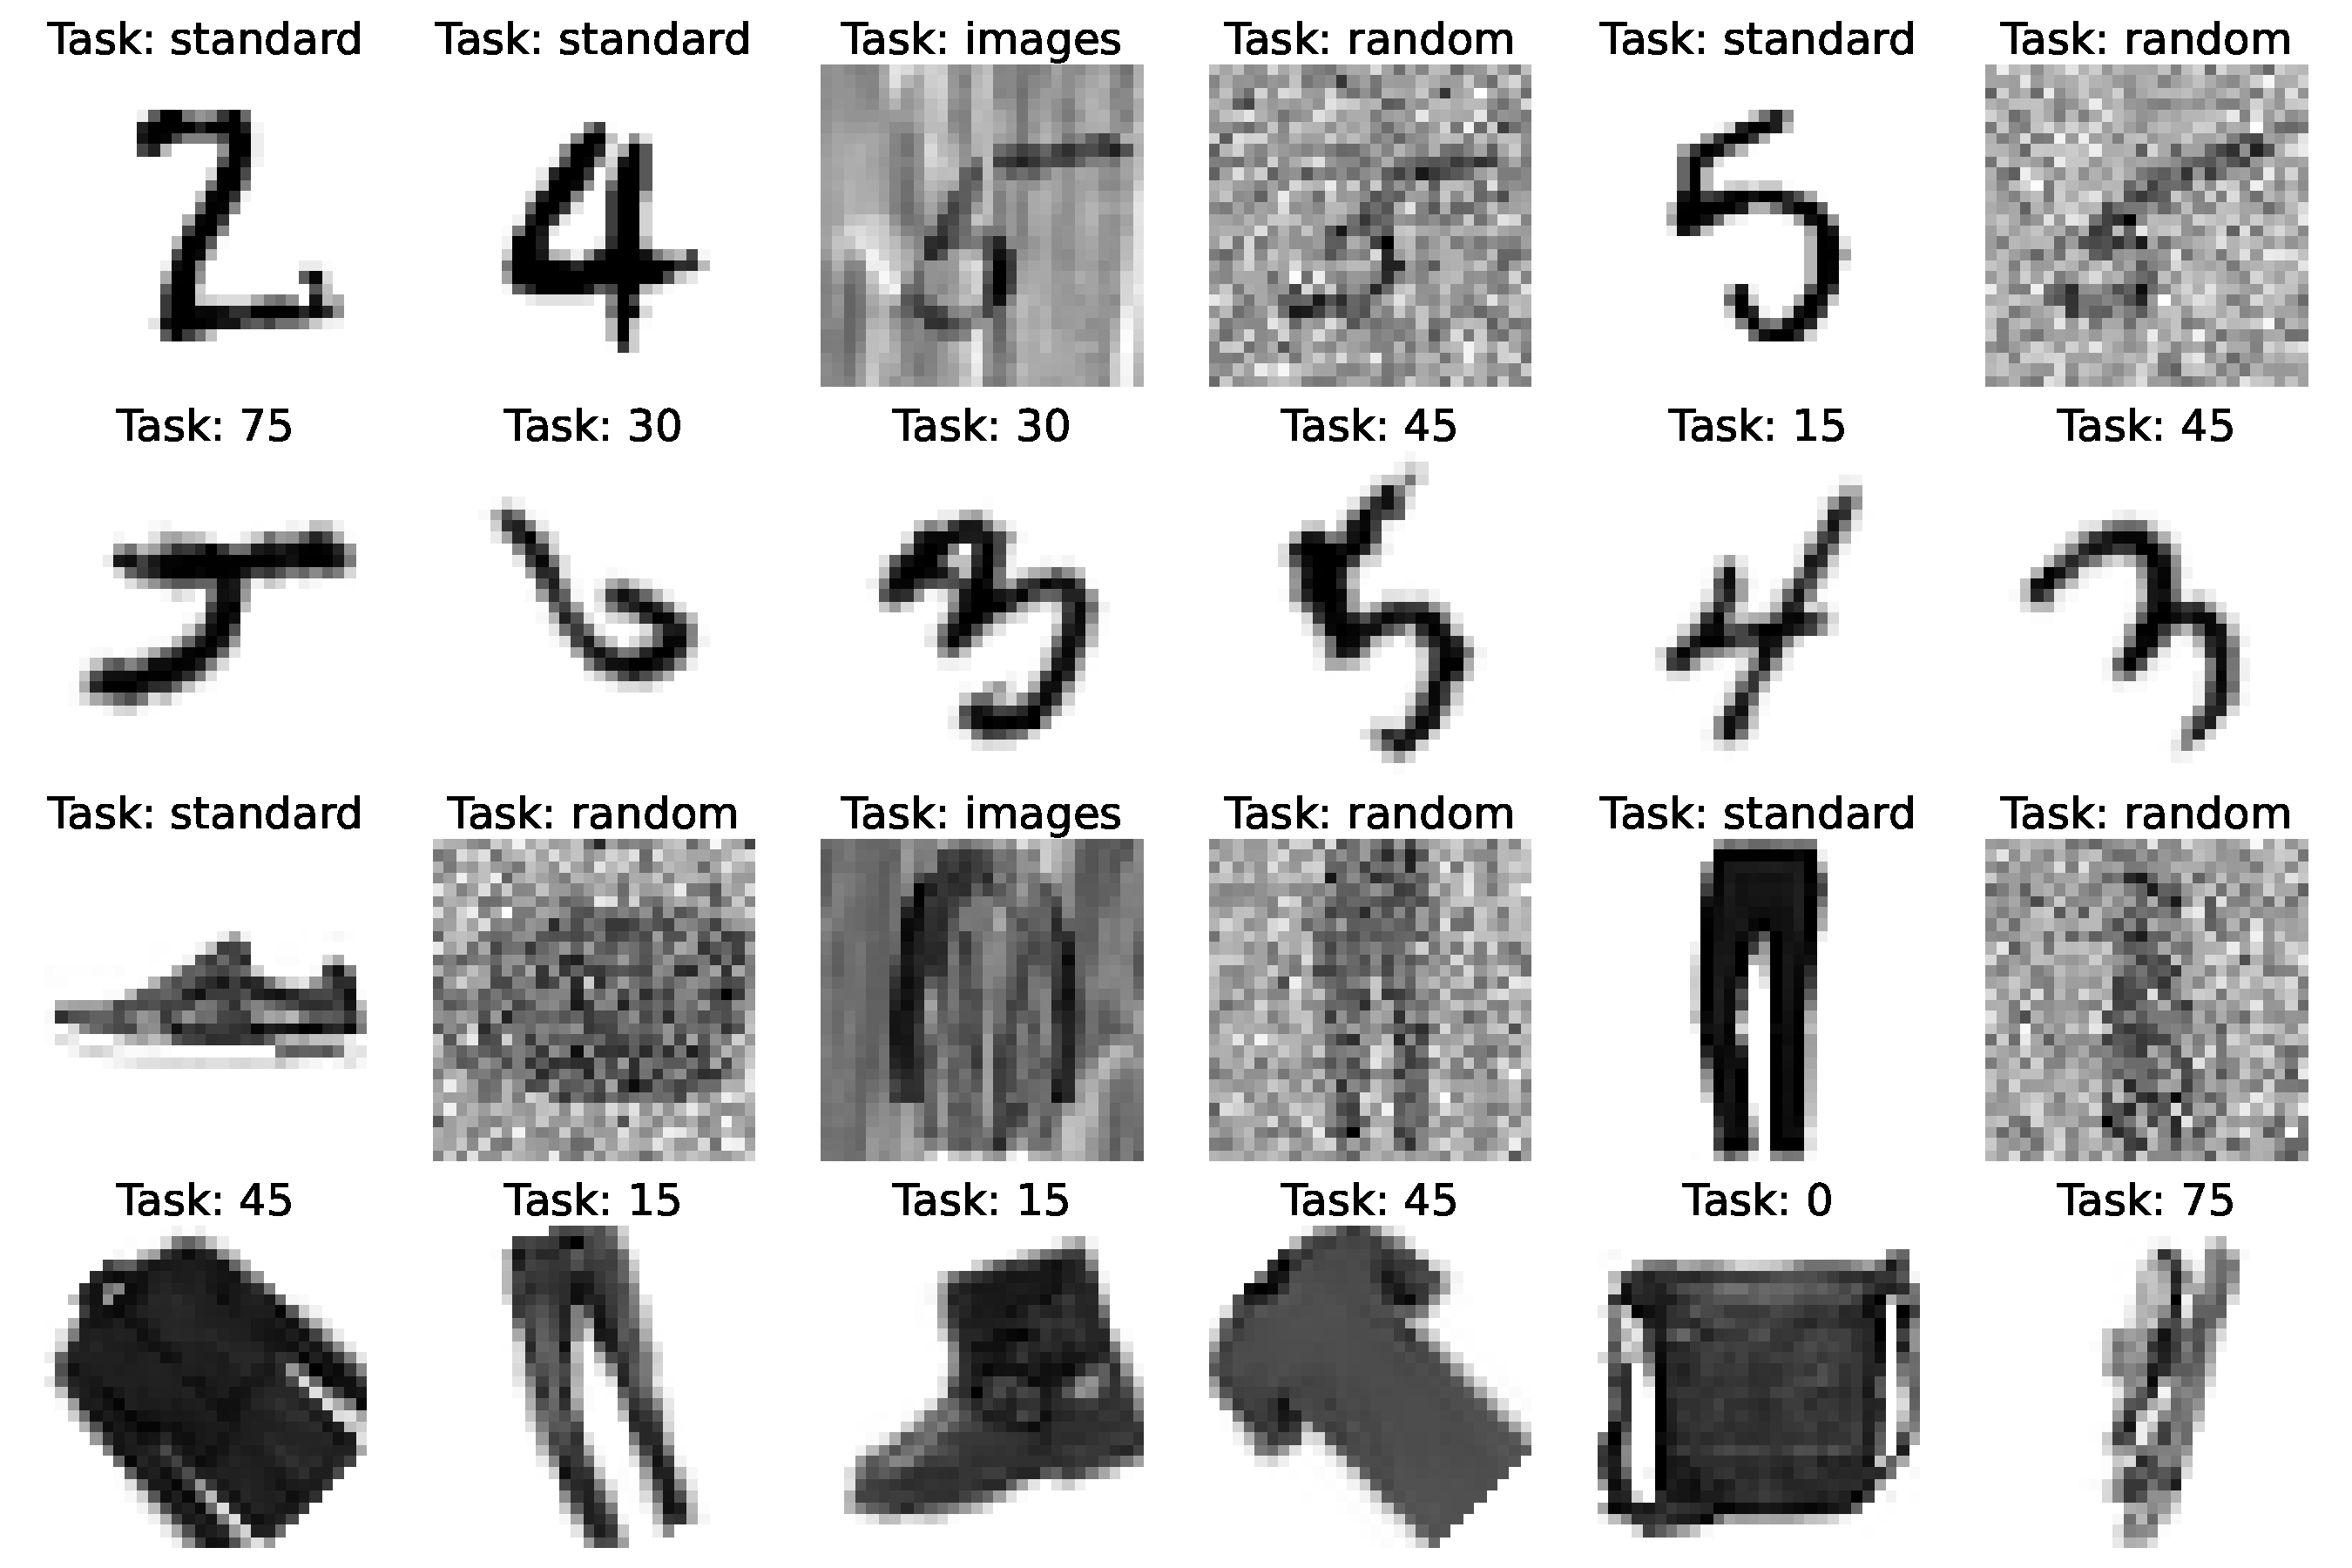
\includegraphics[width=.7\linewidth]{Chapter6/HAIS2022/hais22_datasets.pdf}

\end{frame}

\begin{frame}{Experimentos: Modelos}

      \begin{itemize}
          \item Comparamos cuatro modelos:
          \begin{itemize}
              \item \fmod{ctlNN\_conv}
              \item \fmod{itlNN\_conv}
              \item \fmod{cvxmtlNN\_conv}
              \item \fmod{hsmtlNN\_conv}
          \end{itemize}
          \item Todos están basados en una red convolucional de \texttt{Pytorch} con
          \begin{itemize}
              \item Conv. Layer (10 output channels)
              \item Conv. Layer (20 output channels)
              \item Dropout ($p=0.5$) and Max. Pooling
              \item Fully Connected Layer (320 neurons)
              \item Fully Connected Layer (50 neurons)
          \end{itemize}
          \item Todos los modelos se entrenan con el algoritmo \emph{AdamW}. CV para hiperpar.
          \begin{itemize}
            \item $\alpha$ (weight decay)
            \item $\lambda$ (en el modelo convexo)
          \end{itemize}
      \end{itemize}
  
  \end{frame}

% \begin{frame}
%       \frametitle{Resultados}
%       \centering
%       \scalebox{.9}{
%             \begin{tabular}{l*{4}{c}}
%                 \hline
%                                    &   \fdata{var-MNIST} &   \fdata{rot-MNIST} &   \fdata{var-FMNIST} &   \fdata{rot-FMNIST} \\
%                 \hline
%                  \fmod{ctlNN} &              0.964 &           0.973 &                     0.784 &                  0.834 \\
%                  \fmod{itlNN} &              0.968 &           0.981 &                     0.795 &                  0.873 \\
%                  \fmod{hsNN}  &              0.971 &           0.980  &                    0.770  &                 0.852 \\
%                  \multirow{2}*{\fmod{mtlNN}} &              \fmaxn{0.974} &           \fmaxn{0.984} &                     \fmaxn{0.812} &                  \fmaxn{0.880} \\
%                  & ($\lambda^* = {0.6}$)  & ($\lambda^* = {0.8}$) & ($\lambda^* = {0.6}$)  & ($\lambda^* = {0.6}$) \\
%                  \hline
%             \end{tabular}
%       }
% \end{frame}


\begin{frame}
      \frametitle{Experimentos: Resultados}
  
      % \begin{itemize}
      %     \item The accuracy test scores are computed using majority voting   
      %     \item The categorical cross-entropy test scores are computed using a combination of the outputs (of the $5$ refitted models) 
      % \end{itemize}
  
      \begin{table}[t!]
          \centering
              %\caption{Test Accuracy with Majority Voting.}
              \label{tab:test_accuracy_majority}
          \scalebox{.7}{
          \begin{tabular}{l*{4}{c}}
              \hline
                                 &   \fdata{var-MNIST} &   \fdata{rot-MNIST} &   \fdata{var-FMNIST} &   \fdata{rot-FMNIST} \\
              \hline
              & \multicolumn{4}{c}{accuracy} \\
              \hline
               \fmod{ctlNN} &              0.964 &           0.973 &                     0.784 &                  0.834 \\
               \fmod{itlNN} &              0.968 &           0.981 &                     0.795 &                  0.873 \\
               \fmod{hsmtlNN}  &              0.971 &           0.980  &                    0.770  &                 0.852 \\
               \multirow{2}*{\fmod{cvxmtlNN}} &              \fmaxn{0.974} &           \fmaxn{0.984} &                     \fmaxn{0.812} &                  \fmaxn{0.880} \\
               & ($\lambda^* = {0.6}$)  & ($\lambda^* = {0.8}$) & ($\lambda^* = {0.6}$)  & ($\lambda^* = {0.6}$) \\
               \hline
               & \multicolumn{4}{c}{categorical cross-entropy} \\
              \hline
               \fmod{ctlNN} & 1.274 $\pm$ 0.143  & 1.145 $\pm$ 0.039 & 2.369 $\pm$ 0.183         & 1.757 $\pm$ 0.075      \\
               \fmod{itlNN} & 1.072 $\pm$ 0.029  & 0.873 $\pm$ 0.058 & 2.356 $\pm$ 0.130         & 1.598 $\pm$ 0.042      \\
               \fmod{hsmtlNN}  & 1.087 $\pm$ 0.253  & 0.898 $\pm$ 0.073 & 3.067 $\pm$ 0.888         & 1.888 $\pm$ 0.075      \\
               \multirow{2}*{\fmod{cvxmtlNN}} & \fmaxn{0.924} $\pm$ \fmaxn{0.024}  & \fmaxn{0.831} $\pm$ \fmaxn{0.029} & \fmaxn{2.147} $\pm$ \fmaxn{0.090}         & \fmaxn{1.482} $\pm$ \fmaxn{0.063}      \\
               & ($\lambda^* = {0.6}$)  & ($\lambda^* = {0.8}$) & ($\lambda^* = {0.6}$)  & ($\lambda^* = {0.6}$)      \\
               \hline
              \end{tabular}
          }
      \end{table}
  
  \end{frame}




%%%%%%%%%%%%%%%%%%%%%%%%%%%%%%%%%%%%%%%%%%%%%%%%%%%%%%%%%%%%%%%%%%%%%%%%%%%%%%%%%%%%%%%%
\section{Laplaciano Adaptativo para Aprendizaje Multitarea}

\begin{frame}
      \frametitle{Aprendizaje Multitarea con Regularización Laplaciana}

      \begin{itemize}
            \item La formulación convexa asume que hay una parte común a todas las tareas
            \item Sin embargo, pueden existir distintos grados de relación entre las tareas
            \vfill
            \item Por otra parte, la definición de tareas puede ser arbitraria
            \item Es posible que definamos tareas distintas que realmente son la misma
            \vfill
            \item Una alternativa para el aprendizaje MT es usar una regularización laplaciana de grafo:
            \begin{itemize}
                  \item para mejorar modelos
                  \item para encontrar relaciones entre tareas
            \end{itemize}
      \end{itemize}

\end{frame}

\begin{frame}
      \frametitle{Aprendizaje Multitarea con Regularización Laplaciana}

      \begin{itemize}
            
            \item Consideramos un grafo donde
            \begin{itemize}
                  \item Los nodos representan tareas
                  \item Las aristas y sus pesos representan las relaciones entre las tareas
            \end{itemize}
            \item La matriz de adyacencia $A$ tiene los pesos de las aristas
            \item La matriz de grados $D$ es una matriz diagonal donde
            \begin{myequation*}
                  (D)_{rr} = \sum_{s=1}^\ntasks (A)_{rs}
            \end{myequation*}
            \item La matriz Laplaciana se define como $L = D - A$
      \end{itemize}
      
\end{frame}


\begin{frame}
      \frametitle{Aprendizaje Multitarea con Regularización Laplaciana}

      \begin{itemize}
            \item Dados los modelos para cada tarea definidos como
            \begin{myequation*}
                  \hypf_r(\cdot) = \dotp{w_r}{\cdot} + b_r,
            \end{myequation*}
            definimos la regularización
            \begin{myequation}
                  \nonumber
                  %\label{eq:gl_regularization}
                  \sum_{r=1}^\ntasks \sum_{s=1}^\ntasks (A)_{rs} \norm{w_r - w_s}^2 
              \end{myequation}
            \item Esta regularización se puede expresar como
            \begin{myequation}
                  \nonumber
                  %\label{eq:gl_regularization}
                  \sum_{r=1}^\ntasks \sum_{s=1}^\ntasks (A)_{rs} \norm{w_r - w_s}^2 = \sum_{r=1}^\ntasks \sum_{s=1}^\ntasks (L)_{rs} \dotp{w_r}{w_s} 
              \end{myequation}
              \item ¿Cómo definimos la regularización laplaciana en un espacio de kernel?
      \end{itemize}
      
\end{frame}




\subsection{Laplaciano de Grafo con Métodos de Kernel}

\begin{frame}
      \frametitle{Laplaciano de Grafo con Métodos de Kernel}

      \begin{itemize}
            % \item La regularización Laplaciana penaliza las distancias
            % \item ¿Cómo calcular las distancias en un Espacio de Hilbert con Kernel Reproductor?
            \item Inspirados por el trabajo en~\footfullcite{EvgeniouMP05} proponemos lo siguiente:
            \begin{itemize}
            \item Consideramos el problema de minimización (con $E$ una matriz def. pos.)
            \begin{myequation}
                  \label{eq:mtl_kernel_altext_original}
                  \begin{aligned}
                       & R({u_1, \ldots, u_T}) = \sum_{r=1}^{\ntasks} \sum_{i=1}^{\npertask_r} \lossf(y_i^r, \dotp{u_r}{\phi(x_i^r)}) + \mu \sum_r \sum_s (E)_{rs} \dotp{u_r}{u_s}  \\
                  \end{aligned}
            \end{myequation}
            \item Si usamos el vector $\fv{u}^\intercal = (u_1^\intercal, \ldots, u_\ntasks^\intercal)$ lo expresamos como
            \begin{myequation}
                  \label{eq:mtl_kernel_altext_tensor}
                  \begin{aligned}
                          & R(\myvec{u}) = \sum_{r=1}^{\ntasks} \sum_{i=1}^{\npertask_r} \lossf(y_i^r, \dotp{\myvec{u}}{e_r \otimes \phi(x_i^r)}) + \mu \left(  \myvec{u}^\intercal (E \otimes I) \myvec{u} \right) \\
                  \end{aligned}
              \end{myequation}
              donde $\otimes$ indica el producto tensorial y $e_1, \ldots e_\ntasks$ es la base canónica de $\reals^\ntasks$
              %\item Aquí $E$ es una matriz definida positiva (ej. $E = L$)
            \end{itemize}
      \end{itemize}

\end{frame}

\begin{frame}
      \frametitle{Laplaciano de Grafo con Métodos de Kernel}

      \begin{lemma}\label{lemma:regproblems_kernel}
            Las soluciones $u_1^*, \ldots, u_\ntasks^*$ de~\eqref{eq:mtl_kernel_altext_original}, o equivalentemente la solución $\opt{\fv{u}}$ de~\eqref{eq:mtl_kernel_altext_tensor},    
            se pueden obtener minimizando
            \begin{myequation}
                \nonumber%\label{eq:mtl_kernel_tensor}
                \begin{aligned}
                     & S(\myvec{w}) = \sum_{r=1}^{\ntasks} \sum_{i=1}^{\npertask_r} \lossf(y_i^r, \dotp{\myvec{w}}{(B_r \otimes \phi(x_i^r))}) + \mu  \myvec{w}^\intercal \myvec{w} , \\
                \end{aligned}
            \end{myequation}
            donde $\bm{w} \in \reals^p \otimes \hilbertspace$ con $p \geq \ntasks$ y $B_r$ son las columnas de $B \in \reals^{p \times \ntasks}$, una matriz de rango máximo tal que $\mymat{E}^{-1} = \mymat{B}^\intercal \mymat{B}$.
        \end{lemma}
        El kernel reproductor correspondiente es:
        \begin{myequation}
            \nonumber
            \dotp{B_r \otimes \phi(x_i^r)}{B_s \otimes \phi(x_j^s)} = \left(E^{-1} \right)_{rs} k(x_i^r, x_j^s) 
        \end{myequation}

\end{frame}


\begin{frame}
      \frametitle{Laplaciano de Grafo con Métodos de Kernel y Formulación Convexa}
      \begin{itemize}
            \item Proponemos combinar la formulación convexa con la regularización Laplaciana~\footfullcite{RuizAD20}
            %\item El problema de minimización es
            \begin{myequation}
                  \nonumber%\label{eq:mtl_kernel_altext_original}
                  \begin{aligned}
                       & \sum_{r=1}^{\ntasks} \sum_{i=1}^{\npertask_r} \lossf(y_i^r, \lambda_r \dotp{w}{\phi(x_i^r)} + (1- \lambda_r) \dotp{ v_r}{\phi(x_i^r)}) 
                       + \sum_r \sum_s (I + \mu L)_{rs} \dotp{v_r}{v_s} + \dotp{w}{w}
                  \end{aligned}
            \end{myequation}
            \item Usando esta formulación y el lema anterior proponemos:
            \begin{itemize}
                  \item L1-SVM MT convexa con regularización laplaciana
                  \item L2-SVM MT convexa con regularización laplaciana
                  \item LS-SVM MT convexa con regularización laplaciana
            \end{itemize}
            
      \end{itemize}
      

\end{frame}

\begin{frame}
      \frametitle{Formulación Convexa para L1-SVM MT con Laplaciano}
  
      \begin{block}{Problema Primal - L1-SVM Convexa con Laplaciano}
            \begin{myequation}\nonumber
                  \begin{aligned}
                       & \min_{\fv{v}, \fv{b}, \fv{\xi}, w}
                       &                                             & { C \sum_{r=1}^\ntasks \sum_{i=1}^{\npertask_r} {\xi_i^r}  + \frac{\nu}{2} \sum_{r=1}^\ntasks \sum_{s=1}^T (L)_{rs} \dotp{v_r}{v_s} + \frac{1}{2} \sum_r \norm{{v}_r}^2 + \frac{1}{2} \norm{{w}}^2}                                                                              \\
                       & \text{s.t.}
                       &                                             & y_i^r (\lambda_r (\dotp{w}{\phi({x}_i^r)}) + (1 - \lambda_r) (\dotp{{v}_r}{\psi({x}_i^r})) + b_r) \geq p_i^r - \xi_i^r  ,                                                                                                                                                                            \\
                       &                                             &                                                                                                                                                                                                           & \xi_i^r \geq 0,  \;  i = 1, \dotsc, \npertask_r, \; r=1, \dotsc, \ntasks 
                  \end{aligned}
              \end{myequation}
      \end{block}
      \begin{itemize}
            \item Los hiperparámetros $\lambda_r$ regulan la influencia de cada parte:
            \begin{itemize}
                \item $\lambda_1, \ldots, \lambda_\ntasks=0$: modelos independientes (ITL)
                \item $\lambda_1, \ldots, \lambda_\ntasks=1$: modelo común (CTL)
            \end{itemize}
            \item La matriz laplaciana $L$ establece relaciones entre las partes específicas $v_r$
      \end{itemize}

\end{frame}


\begin{frame}
      \frametitle{Formulación Convexa para L1-SVM MT con Laplaciano}
  
      \begin{block}{Problema Dual - L1-SVM Convexa con Laplaciano}
            \begin{myequation}\nonumber%\label{eq:dual_cvxgl_l1_kernel}
                  \begin{aligned}
                       & \min_{\fv{\alpha}}
                       &                       & \Theta(\fv{\alpha}) = \frac{1}{2} \fv{\alpha}^t \left( \Lambda \fm{Q} \Lambda + \left(\fm{I}_{\nsamples} - \Lambda \right) \fm{\widetilde{Q}} \left(\fm{I}_{\nsamples} - \Lambda \right) \right) \fv{\alpha} - \fv{p} \fv{\alpha}                                                             \\
                       & \text{s.t.}
                       &                       & 0 \leq \alpha_i^r \leq C, \;  i=1,\ldots,m_r, r=1,\ldots,T ,                                                                                                                                                                                                                                  \\
                       &                       &                                                                                                                                                                                                                                   & \sum_{i=1}^{n_r}{\alpha_i^r y_i^r} = 0, \; r=1,\ldots,\ntasks
                  \end{aligned}
              \end{myequation}
      \end{block}
      \begin{itemize}
            \item Usamos la matriz $  \Lambda = \Diag(\overbrace{\lambda_1, \ldots, \lambda_1}^{\npertask_1}, \ldots, \overbrace{\lambda_\ntasks, \ldots, \lambda_\ntasks}^{\npertask_\ntasks}) $
            \item La matriz $Q$ es común entre todas las tareas usando el kernel $k_\phi$ correspondiente a $\phi$
            \item La matriz $\tilde{Q}$ se define usando el kernel: $\widetilde{k}_\psi(x_i^r, x_j^s) = \left( \left(\nu \fm{L} + \fm{I}_\ntasks\right)^{-1} \right)_{rs} k_\psi(x_i^r, x_j^s) $
            % \begin{myequation}
            %       \label{eq:kernelfun_gl_kernel}
            %       \widetilde{k}(x_i^r, x_j^s) = \left( \left(\nu \fm{L} + \fm{I}_\ntasks\right)^{-1} \right)_{rs} k(x_i^r, x_j^s) ,
            %   \end{myequation}
            \item La función de kernel es: 
            $    \widehat{k}({x}_i^r, {x}_j^s) = \lambda_r \lambda_s k_\phi({x}_i^r, {x}_j^s) +  (1-\lambda_r) (1 - \lambda_s) \widetilde{k}_\psi({x}_i^r, {x}_j^s) 
            $
      \end{itemize}

\end{frame}


\begin{frame}
      \frametitle{Formulación Convexa para L2-SVM MT con Laplaciano}
  
      \begin{block}{Problema Primal - L2-SVM Convexa con Laplaciano}
            \begin{myequation}\nonumber
                  \begin{aligned}
                       & \min_{\substack{v_1, \ldots, v_\ntasks ;                                                                                                                                                                                                                                                                                          \\ \substack{b_1, \ldots, b_\ntasks } ; \\ \substack{\fv{\xi}}, w; }}
                       &                                             & { C \sum_{r=1}^\ntasks \sum_{i=1}^{\npertask_r} {(\xi_i^r)^2}  + \frac{\nu}{2} \sum_{r=1}^\ntasks \sum_{s=1}^T (A)_{rs} {\| {v}_r - {v}_s \|}^2 + \frac{1}{2} \sum_r \norm{{v}_r}^2 + \frac{1}{2} \norm{{w}}^2}                                                                              \\
                       & \text{s.t.}
                       &                                             & y_i^r (\lambda_r (\dotp{w}{\phi({x}_i^r)}) + (1 - \lambda_r) (\dotp{{v}_r}{\psi({x}_i^r})) + b_r) \geq p_i^r - \xi_i^r  ;
                  \end{aligned}
              \end{myequation}
      \end{block}
      \begin{block}{Problema Dual - L2-SVM Convexa con Laplaciano}
            \begin{myequation}\nonumber
                  \begin{aligned}
                       & \min_{\fv{\alpha}}
                       &                       & \Theta(\fv{\alpha}) = \frac{1}{2} \fv{\alpha}^t \left\lbrace  \left( \Lambda \fm{Q} \Lambda + \left(\fm{I}_{\nsamples} - \Lambda \right) \fm{\widetilde{Q}} \left(\fm{I}_{\nsamples} - \Lambda \right) \right) + \frac{1}{C} \fm{I}_\nsamples \right\rbrace \fv{\alpha} - \fv{p} \fv{\alpha}                                                            \\
                       & \text{s.t.}
                       &                       & 0 \leq \alpha_i^r, \;  i=1,\ldots,m_r,\; r=1,\ldots,T ,   \;  \sum_{i=1}^{n_r}{\alpha_i^r y_i^r} = 0, \; r=1,\ldots,T
                  \end{aligned}
              \end{myequation}
      \end{block}
      

\end{frame}

\begin{frame}
      \frametitle{Formulación Convexa para LS-SVM MT con Laplaciano}
  
      \begin{block}{Problema Primal - LS-SVM Convexa con Laplaciano}
            \begin{myequation}\nonumber
                  \begin{aligned}
                       & \min_{\substack{v_1, \ldots, v_\ntasks ;                                                                                                                                                                                                                                                                                          \\ \substack{b_1, \ldots, b_\ntasks } ; \\ \substack{\fv{\xi}}, w; }}
                       &                                             & { C \sum_{r=1}^\ntasks \sum_{i=1}^{\npertask_r} {(\xi_i^r)^2}  + \frac{\nu}{2} \sum_{r=1}^\ntasks \sum_{s=1}^T (A)_{rs} {\| {v}_r - {v}_s \|}^2 + \frac{1}{2} \sum_r \norm{{v}_r}^2 + \frac{1}{2} \norm{{w}}^2}                                                                              \\
                       & \text{s.t.}
                       &                                             & y_i^r (\lambda_r (\dotp{w}{\phi({x}_i^r)}) + (1 - \lambda_r) (\dotp{{v}_r}{\psi({x}_i^r})) + b_r) = p_i^r - \xi_i^r 
                  \end{aligned}
              \end{myequation}
      \end{block}
      \begin{block}{Problema Dual - LS-SVM Convexa con Laplaciano}
            \begin{myequation}\nonumber%\label{eq:dual_cvxgl_ls_kernel}
                  \begin{aligned}
                      \left[
                          \begin{array}{c|c}
                              \fv{0}_{\ntasks \times \ntasks} & \fm{A}^\intercal \fm{y}                                                                                                                                                         \\
                              \hline
                              \fm{y} \fm{A}                   & \left( \Lambda \fm{Q} \Lambda + \left(\fm{I}_{\nsamples} - \Lambda \right) \fm{\widetilde{Q}} \left(\fm{I}_{\nsamples} - \Lambda \right) \right) + \frac{1}{C} \fm{I}_\nsamples
                          \end{array}
                          \right]
                      \begin{bmatrix}
                          b_1       \\
                          \vdots    \\
                          b_\ntasks \\
                          \fv{\alpha}
                      \end{bmatrix}
                      =
                      \begin{bmatrix}
                          \fv{0}_\ntasks \\
                          \fv{p}
                      \end{bmatrix}
                  \end{aligned}
              \end{myequation}
      \end{block}
      

\end{frame}

\subsection{Algoritmo Adaptativo para Laplaciano de Grafo}

\begin{frame}
      \frametitle{Algoritmo Adaptativo para Laplaciano de Grafo}

      \begin{itemize}
            \item La selección de la matriz de adyacencia $A$ (y la respectiva $L$) es determinante
            \item Proponemos~\footfullcite{RuizAD21_hais} un método para la selección automática de $A$
            \item Tiene que tener las siguientes restricciones:
            \begin{itemize}
                  \item $A$ es simétrica
                  \item $(A)_{rs} \geq 0$, $r, s=1, \ldots, \ntasks$.
                  \item $\sum_{s=1} (A)_{rs} = 1$
              \end{itemize}
            %\item Se puede escoger usando conocimiento experto del problema
            %\item Proponemos un algoritmo para aprender la matriz $A$ de forma automática
            \item La entropía de cada fila $\fv{a}^r$ es: $H(\fv{a}^r) = \sum_{s=1}^\ntasks (A)_{rs} \log((A)_{rs})$
            %\item Definimos la entropía de $A$ como: $H(A) = \sum_{r=1}^\ntasks H(\fv{a}^r)$
            \item Interpretación:
            \begin{itemize}
                  \item $\sum_{r=1}^\ntasks H(\fv{a}^r) $ es máxima si $A$ es constante, $A = \frac{1}{\ntasks} \fv{1}_\ntasks \fv{1}_\ntasks^\intercal$
                  \item $\sum_{r=1}^\ntasks H(\fv{a}^r) $ es mínima si $A$ es la identidad, $A = I_\ntasks$ 
            \end{itemize}
            
            % \item Proponemos un algoritmo para aprender la matriz de forma automática:
            % \begin{itemize}
            %       \item Empezamos con un enfoque agnóstico: $A$ constante
            %       \item Se calculan los parámetros $\opt{v_r}$ en cada tarea
            %       \item Se calculan las distancias entre tareas para determinar su relación
            %       \item Actualizamos la matriz $A$: $A_{rs} \propto \frac{1}{\norm{v_r - v_s}}$
            % \end{itemize}
      \end{itemize}

\end{frame}


\begin{frame}
      \frametitle{Algoritmo Adaptativo para Laplaciano de Grafo}

      \begin{block}{Problema para Algoritmo Adaptativo}
            \begin{myequation}\nonumber %\label{eq:adapcvxgl_general_problem}
                  \begin{aligned}
                       & \min_{\substack{w, \fv{v}, \fv{b};                                                                                                                                                                                                                                                                                                                              \\  A \in {(\reals_{\geq 0})}^{\ntasks \times \ntasks},  \\ \fm{A} \fv{1}_\ntasks = \fv{1}_\ntasks}}
                       &                                       & C \sum_{r=1}^\ntasks \sum_{i=1}^{\npertask_r} {\lossf(\lambda_r \dotp{w}{\phi({x}_i^r)} + (1 - \lambda_r) \dotp{{v}_r}{\psi({x}_i^r)} + b_r, y_i^r)}                                                                                                                                                                       \\
                       &                                       &                                                                                                                                                      & \quad + \frac{\nu}{2} \sum_{r=1}^\ntasks \sum_{s=1}^\ntasks (A)_{rs} \norm{{v}_r - v_{s}}^2 + \frac{1}{2} \sum_{r=1}^\ntasks \norm{{v}_r}^2 + \frac{1}{2}\norm{{w}}^2 \\
                       &                                       &                                                                                                                                                      & \quad- \mu \sum_{r=1}^\ntasks H(\fv{a}^r) 
                  \end{aligned}
              \end{myequation}
            \end{block}

\end{frame}


\begin{frame}
      \frametitle{Algoritmo Adaptativo para Laplaciano de Grafo}

      \begin{itemize}
            \item Para minimizar este problema alternamos los siguientes pasos:
            \begin{itemize}
                  \item Fijamos $A$ y minimizamos en $w, \fv{v}, \fv{b}$: %resolvemos el problema dual (y obtenemos $\opt{\fv{\alpha}}$) correspondiente a
                  \begin{myequation}\nonumber %\label{eq:adapcvxgl_general_problem}
                        \begin{aligned}
                             & \min_{w, \fv{v}, \fv{b}}
                             &                                       & C \sum_{r=1}^\ntasks \sum_{i=1}^{\npertask_r} {\lossf(\lambda_r \dotp{w}{\phi({x}_i^r)} + (1 - \lambda_r) \dotp{{v}_r}{\psi({x}_i^r)} + b_r, y_i^r)}                                                                                                                                                                       \\
                             &                                       &                                                                                                                                                      & \quad + \frac{\nu}{2} \sum_{r=1}^\ntasks \sum_{s=1}^\ntasks (A)_{rs} \norm{{v}_r - v_{s}}^2 + \frac{1}{2} \sum_{r=1}^\ntasks \norm{{v}_r}^2 + \frac{1}{2}\norm{{w}}^2 
                        \end{aligned}
                    \end{myequation}
                  % \begin{myequation}\nonumber%\label{eq:dual_cvxgl_l1_kernel}
                  %       \begin{aligned}
                  %            & \min_{\fv{\alpha}}
                  %            &                       & \Theta(\fv{\alpha}) = \frac{1}{2} \fv{\alpha}^t \left( \Lambda \fm{Q} \Lambda + \left(\fm{I}_{\nsamples} - \Lambda \right) \fm{\widetilde{Q}} \left(\fm{I}_{\nsamples} - \Lambda \right) \right) \fv{\alpha} - \fv{p} \fv{\alpha}                                                             \\
                  %            & \text{s.t.}
                  %            &                       & 0 \leq \alpha_i^r \leq C, \;  i=1,\ldots,m_r, r=1,\ldots,T ,                                                                                                                                                                                                                                  \\
                  %            &                       &                                                                                                                                                                                                                                   & \sum_{i=1}^{n_r}{\alpha_i^r y_i^r} = 0, \; r=1,\ldots,T .
                  %       \end{aligned}
                  %   \end{myequation}
                  \item Fjamos $w, \fv{v}, \fv{b}$ y minimizamos en $A$: 
                  \begin{myequation}\nonumber
                        \begin{aligned}
                            \min_{\substack{A \in {(\reals_{\geq 0})}^{\ntasks \times \ntasks}, \\ \fm{A} \fv{1}_\ntasks = \fv{1}_\ntasks}}
                            J(A) = \frac{\nu}{2} \sum_{r=1}^\ntasks \sum_{s=1}^\ntasks (A)_{rs} \norm{{v}_r - v_{s}}^2 - \mu \sum_{r=1}^\ntasks H(\fv{a}^r)
                        \end{aligned}
                    \end{myequation}
            \end{itemize}
            
      \end{itemize}

\end{frame}

% \begin{frame}
%       \frametitle{Algoritmo Adaptativo para Laplaciano de Grafo}

%       \begin{itemize}
%             \item Si sabemos las distancias $\norm{v_r - v_s}^2$, la solución es
%             \begin{myequation}\nonumber%\label{eq:update_A}
%                   (A)_{rs} = \frac{\exp{-\frac{\nu}{\mu} \norm{{v}_r - {v}_s}^2 } }{\sum_t \exp{-\frac{\nu}{\mu}  \norm{{v}_r - {v}_t}^2} }
%               \end{myequation}
%             \item ¿Cómo calculamos estas distancias?
%             \begin{itemize}
%                   \item Con la matriz $ \widetilde{{\fm{Q}^{rs}}}$ correspondiente a la función
%             \begin{myequation}
%                   \nonumber%\label{eq:dot_computation_kernel}
%                   \widetilde{{k^{rs}}}(x_i^t, x_j^\tau) = (\fm{I}_\ntasks + \nu \fm{L})^{-1}_{rt} (\fm{I}_\ntasks + \nu \fm{L})^{-1}_{s\tau} k_\psi(x_i^t, x_j^\tau)
%               \end{myequation}
%             \item Los productos interiores son
%             \begin{myequation}\nonumber%\label{eq:dot_computation_matrix}
%                   \dotp{v_r}{v_s} = \fv{\alpha}^\intercal \left(\fm{I}_{\nsamples} - \Lambda \right) \widetilde{{\fm{Q}^{rs}}} \left(\fm{I}_{\nsamples} - \Lambda \right) \fv{\alpha}
%               \end{myequation}
%               \item Las distancias son entonces
%               \begin{myequation}\nonumber%\label{eq:distance_computation_matrix}
%                   \norm{v_r - v_s}^2 = \fv{\alpha}^\intercal \left(\fm{I}_{\nsamples} - \Lambda \right) (\widetilde{{\fm{Q}^{rr}}} + \widetilde{{\fm{Q}^{ss}}} - 2\widetilde{{\fm{Q}^{rs}}}) \left(\fm{I}_{\nsamples} - \Lambda \right) \fv{\alpha}
%               \end{myequation}
%             \end{itemize}     
%       \end{itemize}

% \end{frame}

\begin{frame}

      \scalebox{0.9}{
      \begin{algorithm}[H]
            \caption{Algoritmo para laplaciano adaptativo.}
            \DontPrintSemicolon
            \KwInput{$(X, y) = \set{(x_i^r, y_i^r), i=1, \ldots, \npertask_r; r=1, \ldots, \ntasks}$ \tcp*{Data}}
            % \KwOutput{$\fv{\alpha}^*$ \tcp*{Optimal dual coefficients}}
            % \KwOutput{$\fm{A}^*$ \tcp*{Optimal adjacency matrix}}
            % \KwData{params = $\set{C, \lambda, \nu, \mu, \sigma_\phi, \sigma_\psi (, \epsilon)}$ \tcp*{Hyperparameters}}
            %   $Q_\phi$ = ComputeKernelMatrix($(X, y)$, $\sigma_\phi$) \\
            %   $Q_\psi$ = ComputeKernelMatrix($(X, y)$, $\sigma_\psi$) \\
            %$o^\text{old}$ = $\infty$ \\
            $A = A_0$ \tcp*{Constant matrix}
            \While{True}{
                $L_\text{inv}$ $\gets$ getInvLaplacian($\fm{A}$) \tcp*{Step 0}
                $\alpha_\text{opt}$ $\gets$ solveDualProblem($(X, y)$, $L_\text{inv}$, params) \tcp*{Step 1}
                $o$ $\gets$ computeObjectiveValue($(X, y)$, $L_\text{inv}$, $\alpha_\text{opt}$) \tcp*{Objective function value}
                \If{$o^{old} - o \leq \delta_\text{tol}$}{break \tcp*{Exit condition}}
                %$o^{old} \gets o$ \\
                % \If{$J_\text{obj}^old - J_\text{obj} \geq \delta_\text{\tol}$}{
                %     break \\
                % }
                $D$ $\gets$ computeDistances($(X, y)$, $L_\text{inv}$, $\alpha_\text{opt}$) \tcp*{Step 2}
                $A$ $\gets$ updateAdjMatrix($D$, params) \tcp*{Step 3}
            }
            \Return{$\alpha_\text{opt}, A$}
            % \caption{Adaptive \acrshort{gl} algorithm.}
            % \label{alg:adapgl}
        \end{algorithm}}
      % \begin{itemize}
      %       \item Step 0: invert the matrix $(I_\ntasks + \nu L)$
      %       \item Step 1: minimize the Problema Dual to obtain $\alpha^*$
      %       \item Step 2: compute the distances $\norm{v_r - v_s}^2$ between task parameters
      %       \item Step 3: update the adjacency matrix $A$ using~\eqref{eq:update_A}
      % \end{itemize}

\end{frame}


\begin{frame}
      \frametitle{Experimentos Sintéticos: Problemas}

      \begin{itemize}
            \item Definimos problemas donde las tareas están agrupadas en clusters
            \begin{itemize}
                  \item Definimos $\tau$ tareas subyacentes (clusters) usando las funciones  $f_r, r=1, \ldots, \tau$
                  \item La función de regresión la usamos como frontera de clasificación
                  \item En cada una definimos $T_r$ tareas virtuales, $r=1, \ldots, \tau$ (las que ven los modelos)
            \end{itemize}
      \end{itemize}    
      \vfill
      \centering
              %\caption{Test Accuracy with Majority Voting.}
              \label{tab:test_accuracy_majority}
          \scalebox{.7}{
          \begin{tabular}{l*{5}{c}}
            \toprule
            %& \multicolumn{3}{c}{Tarea Real 1} \\
                                 &   $\tau$ &   $f_r$  & $T_r$  & Total tareas virtuales  \\
              \midrule
               \multirow{3}{*}{\fdata{regClusters0}, \fdata{clasClusters0}} & \multirow{3}{*}{3} & $f_1(x) = x^2$ & 2 & \multirow{3}{*}{7}\\
               & & $f_2(x) = \sin(10x)$ & 3 & \\ 
             & & $f_3(x) = x^3$ & 2  & \\ 
             \midrule
               \multirow{2}{*}{\fdata{regClusters1}, \fdata{clasClusters1}} & \multirow{2}{*}{2} & $f_1(x) = x^2$ & 5 & \multirow{2}{*}{7}\\
               & & $f_2(x) = \sin(10x)$ & 2 & \\ 
             \midrule
               \multirow{2}{*}{\fdata{regClusters2}, \fdata{clasClusters2}} & \multirow{2}{*}{2} & $f_1(x) = \sin(10x)$ & 4 & \multirow{2}{*}{5}\\
               & & $f_2(x) = x^3$ & 1 & \\ 
            %  \midrule
            %   \multirow{2}{*}{\fdata{regClusters1}, \fdata{clasClusters1}} & \multirow{2}{*}{2} & 5 \\
            %    & & 2 \\ 
            %  \midrule
            %   \multirow{2}{*}{\fdata{regClusters2}, \fdata{clasClusters2}} & \multirow{2}{*}{2} & 4 \\
            %    & & 1 \\ 
            %    \fdata{regClusters1}, \fdata{clasClusters1} &              0.968 &           0.981 &                     0.795 \\
            %    \fdata{regClusters2}, \fdata{clasClusters2}  &              0.971 &           0.980  &                    0.770  \\
               \bottomrule
              \end{tabular}
          }
      

\end{frame}


\begin{frame}
      \frametitle{Experimentos Sintéticos: \fdata{clusters0}}

      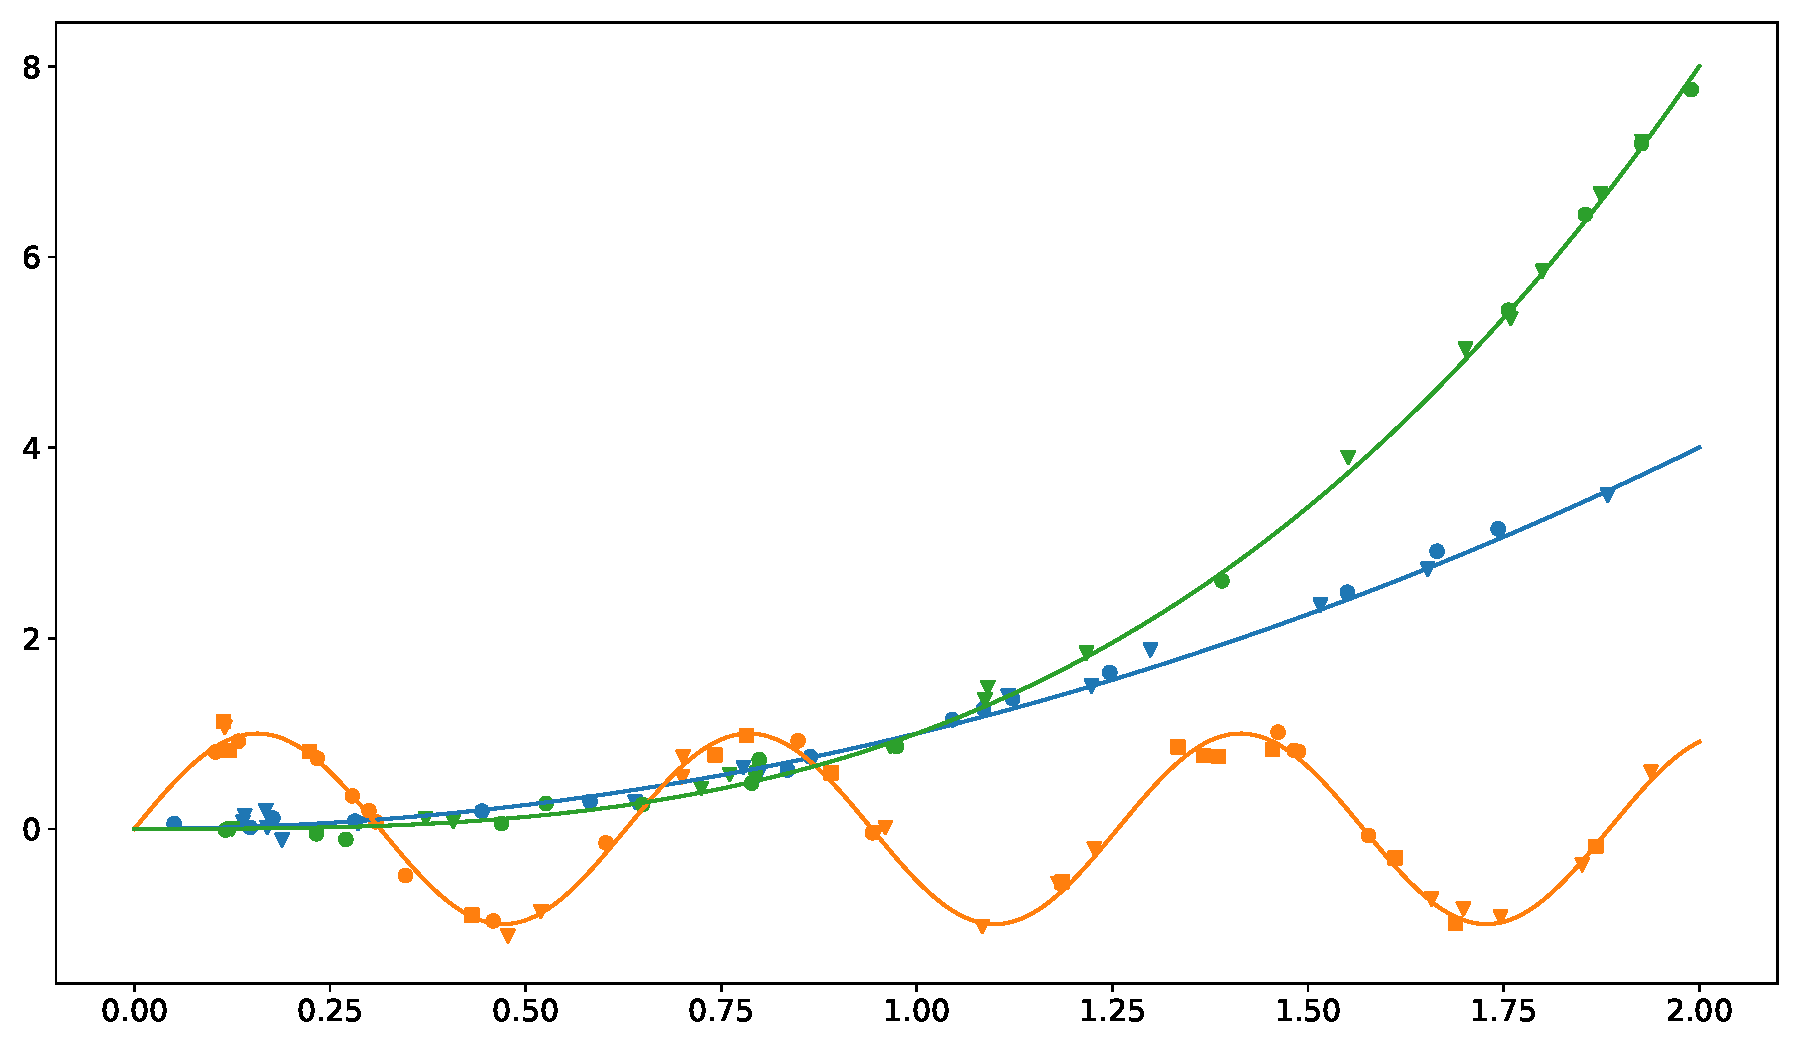
\includegraphics[width=.5\textwidth]{Chapter6/IGPL2022/regClusters__0.pdf}%
      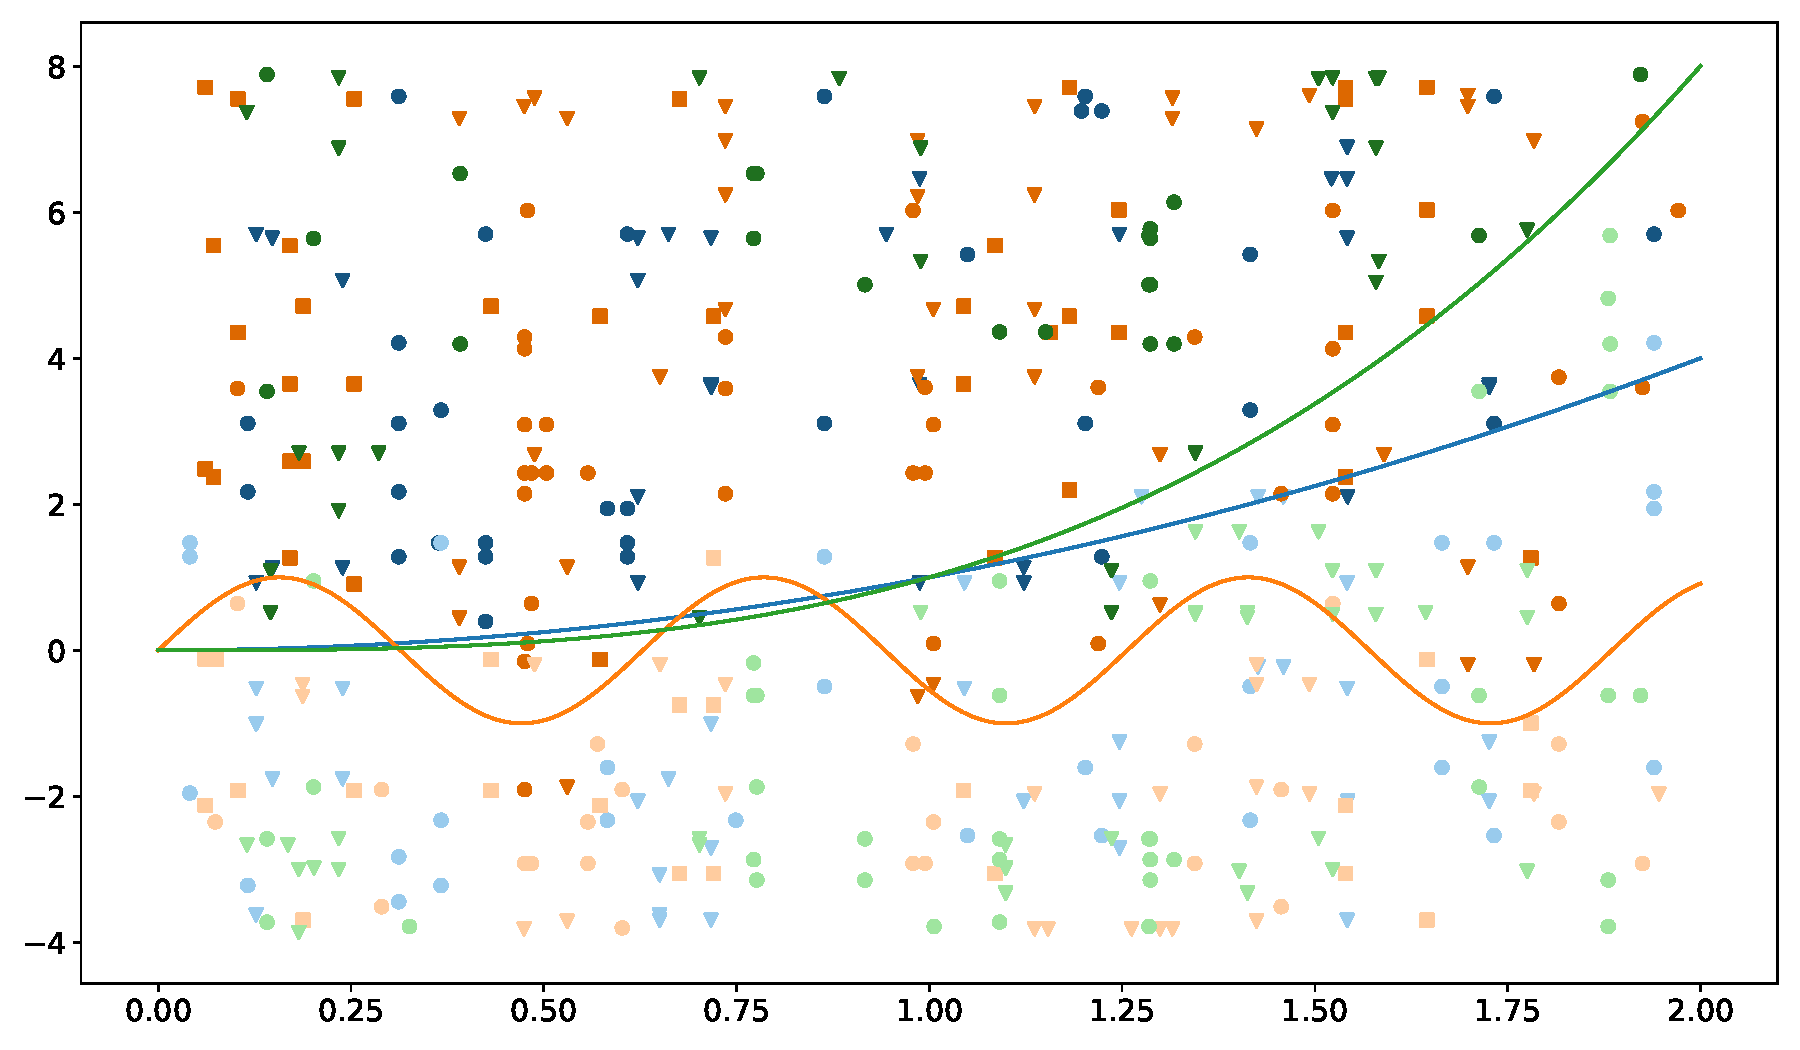
\includegraphics[width=.5\textwidth]{Chapter6/IGPL2022/clasClusters__0.pdf}
      \begin{itemize}
            \item Gráficas de \fdata{regClusters0} y \fdata{clasClusters0}
            %\item Tenemos tres clusters (o tareas )
      \end{itemize}    
      % \begin{figure}
      % \begin{subfigure}[b]{0.49\textwidth}
      %       \centering
      %       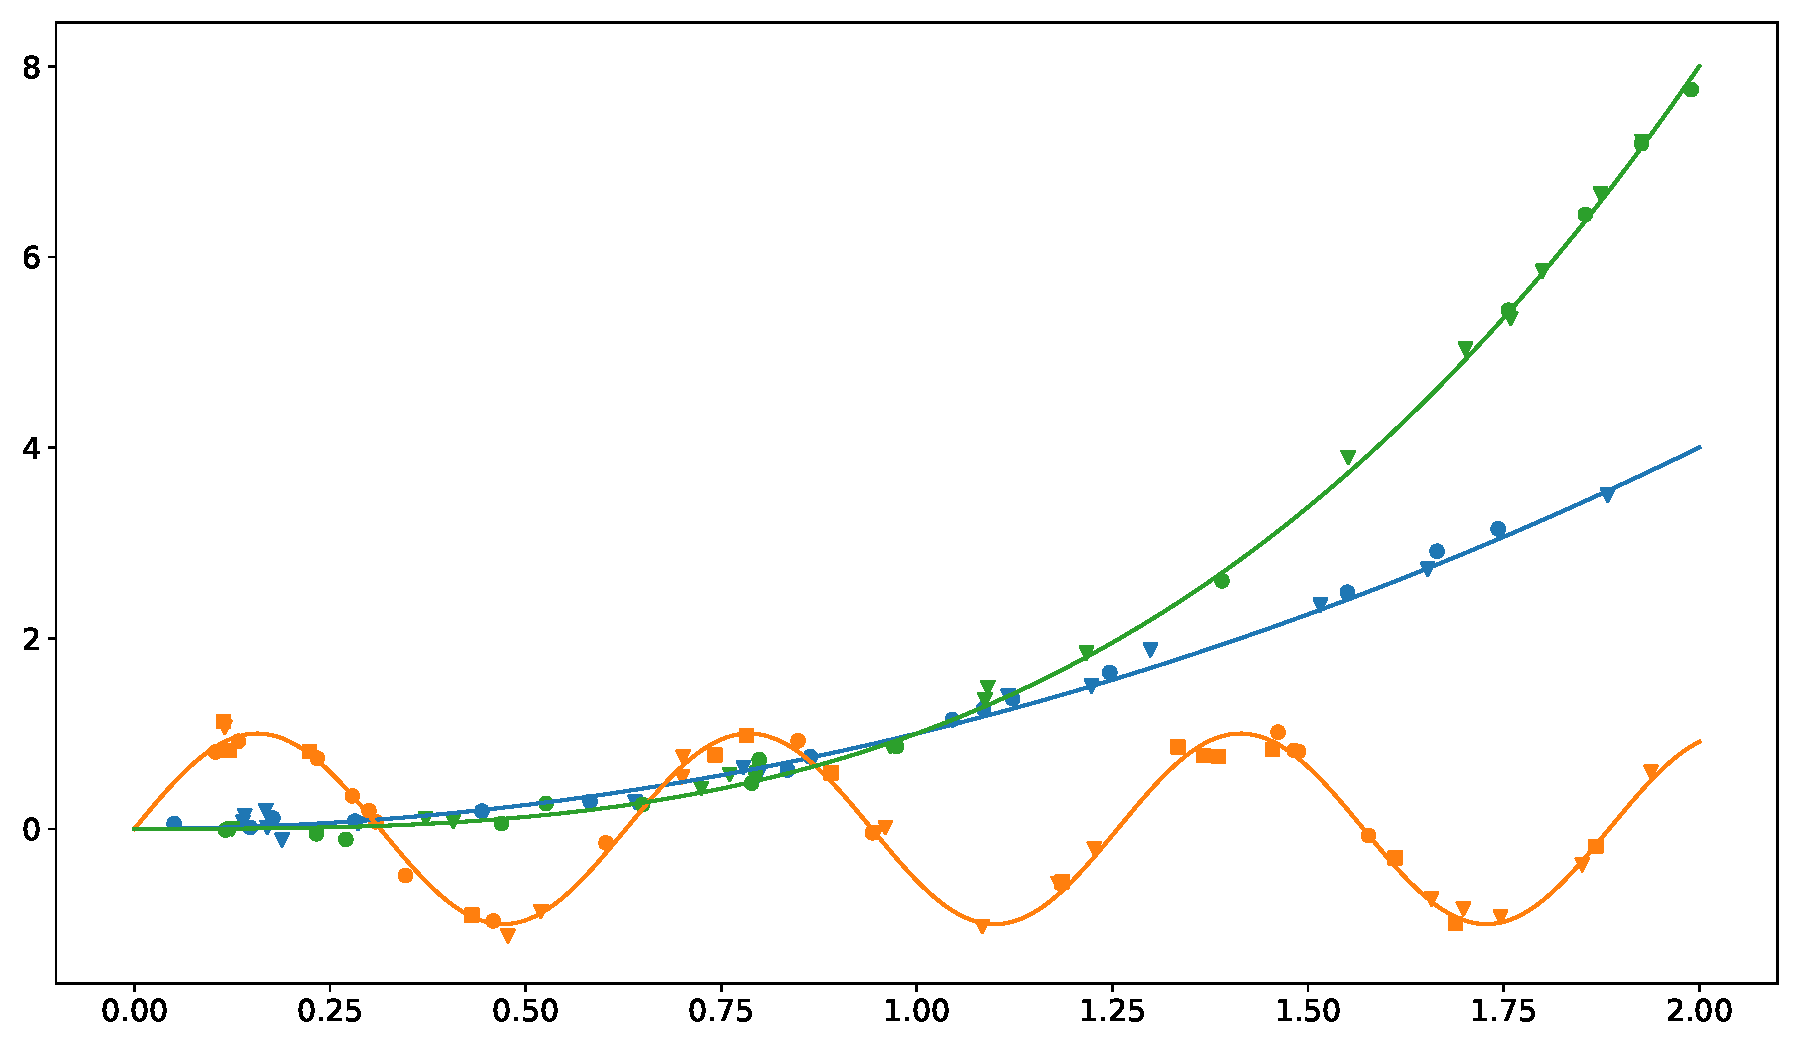
\includegraphics[width=\textwidth]{Chapter6/IGPL2022/regClusters__0.pdf}
      %       \caption{\fdata{regClusters0}.}
      %       % \label{regClusters0}
      % \end{subfigure}
      % \hfill
      % \begin{subfigure}[b]{0.49\textwidth}
      %       \centering
      %       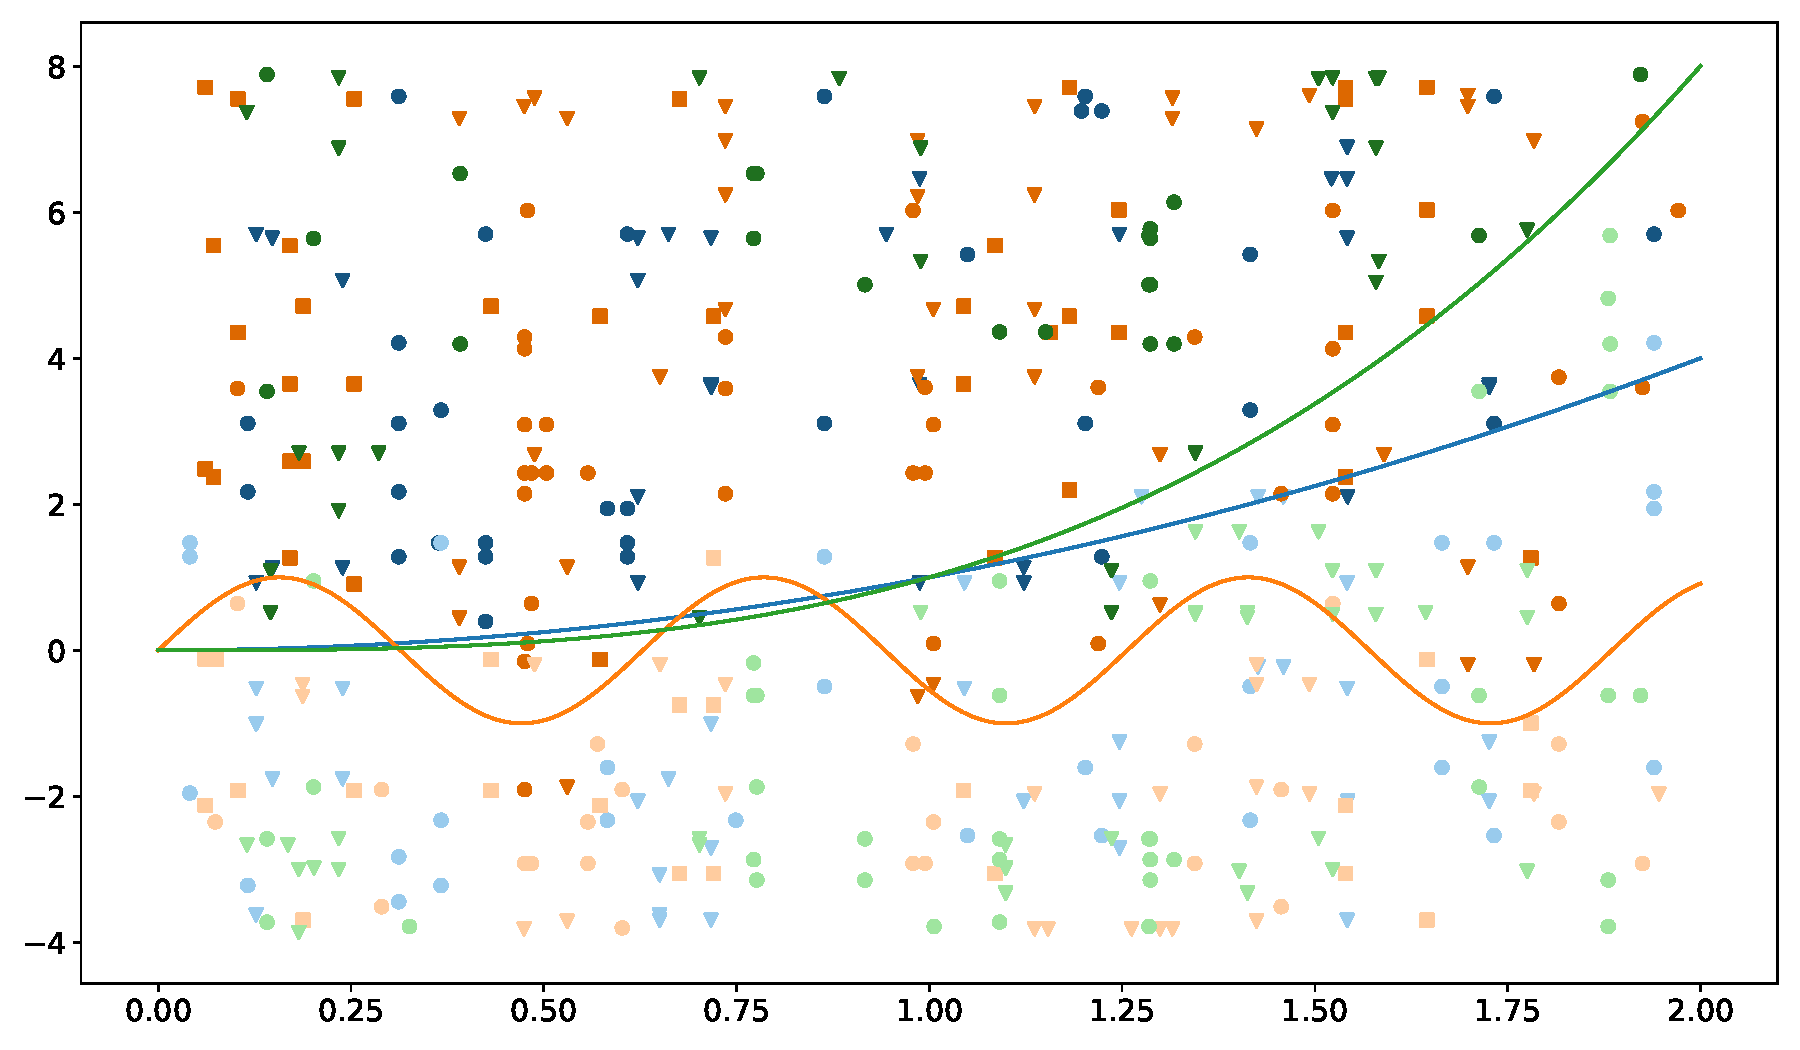
\includegraphics[width=\textwidth]{Chapter6/IGPL2022/clasClusters__0.pdf}
      %       \caption{\fdata{clasClusters0}.}
      %       %\label{clasClusters0}
      % \end{subfigure}
      % \end{figure}

\end{frame}

% \begin{frame}
%       \frametitle{Experimentos Sintéticos: Problemas}

%       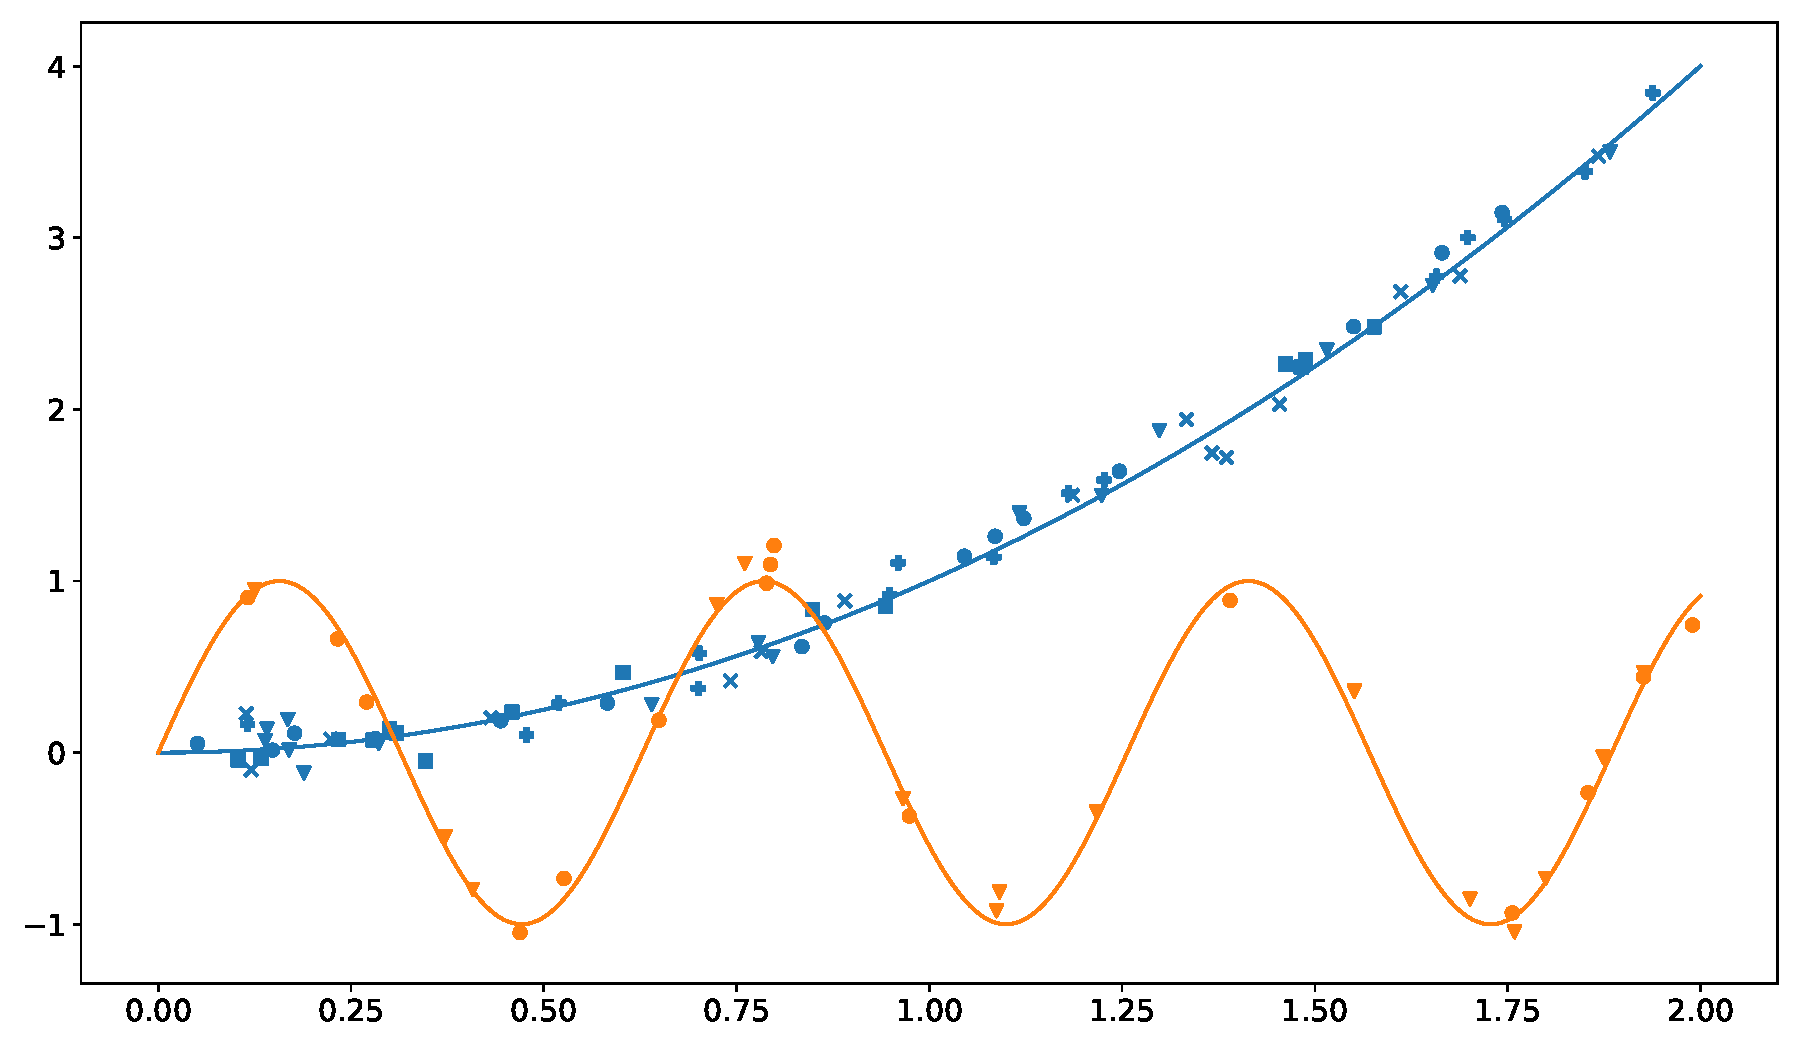
\includegraphics[width=.5\textwidth]{Chapter6/IGPL2022/regClusters__1.pdf}%
%       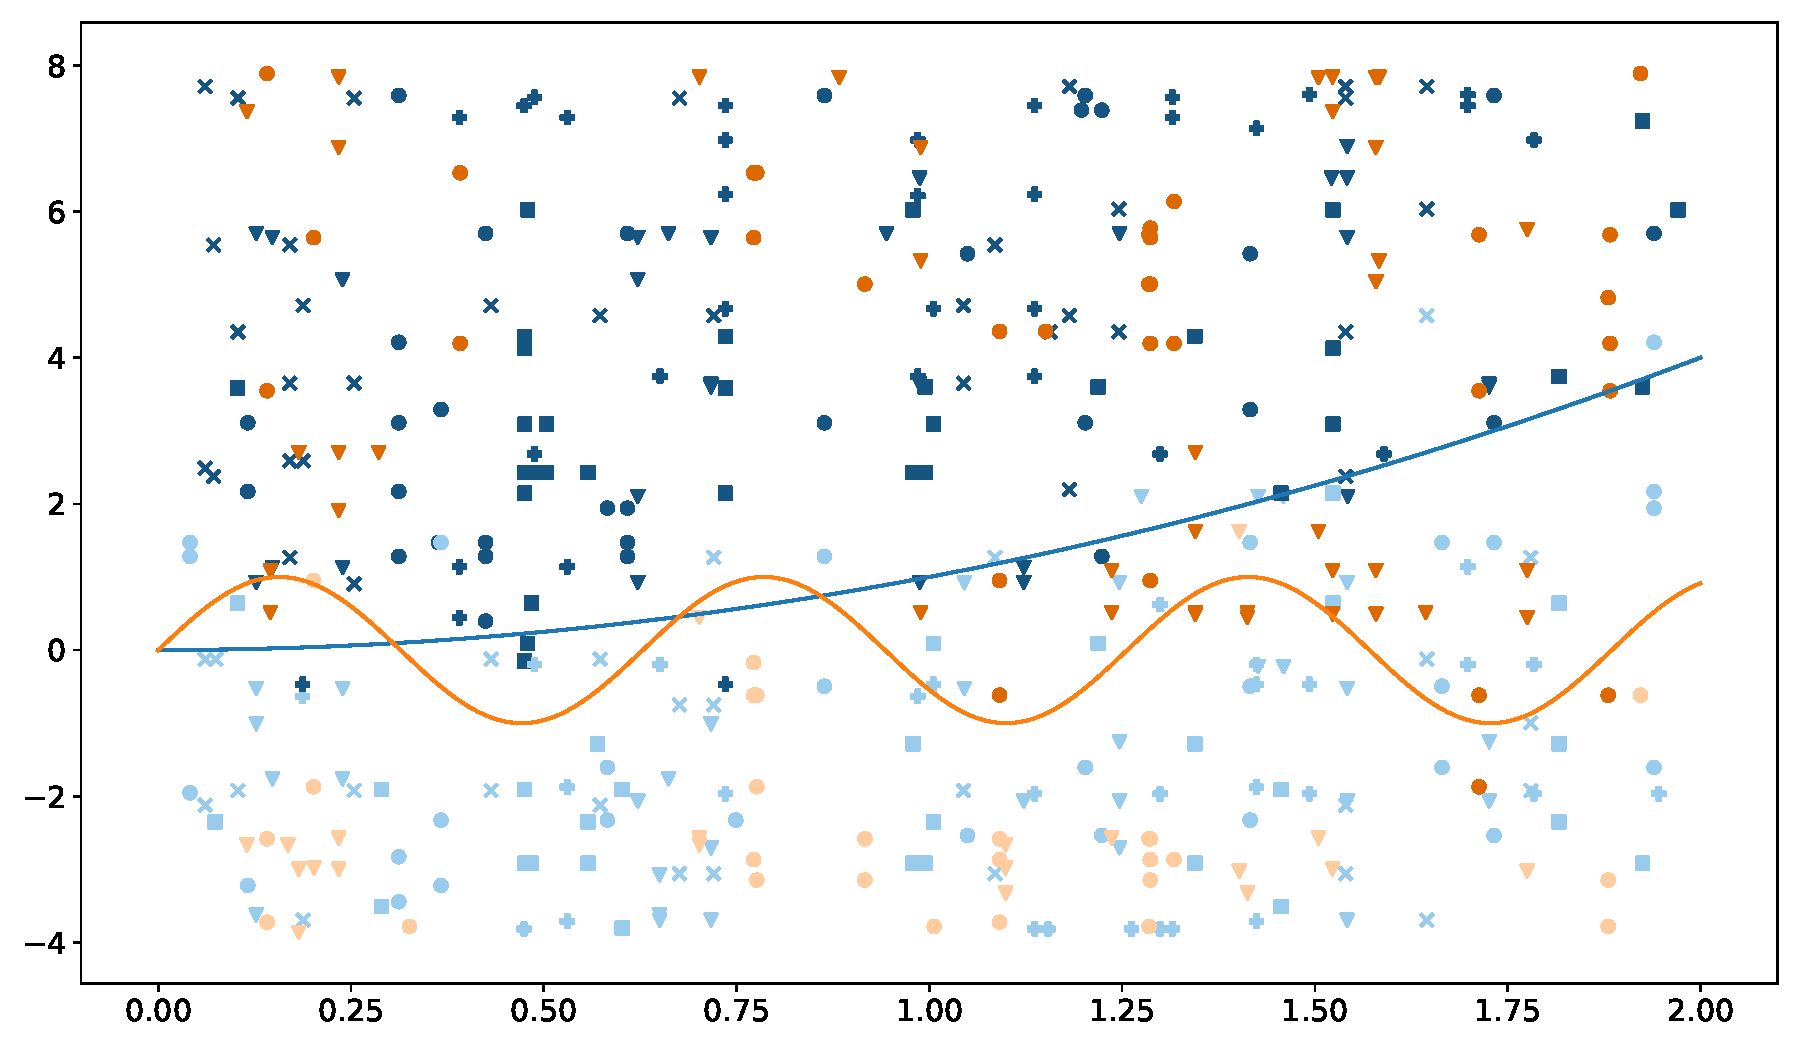
\includegraphics[width=.5\textwidth]{Chapter6/IGPL2022/clasClusters__1.pdf}
%       % \begin{figure}
%       % \begin{subfigure}[b]{0.49\textwidth}
%       %       \centering
%       %       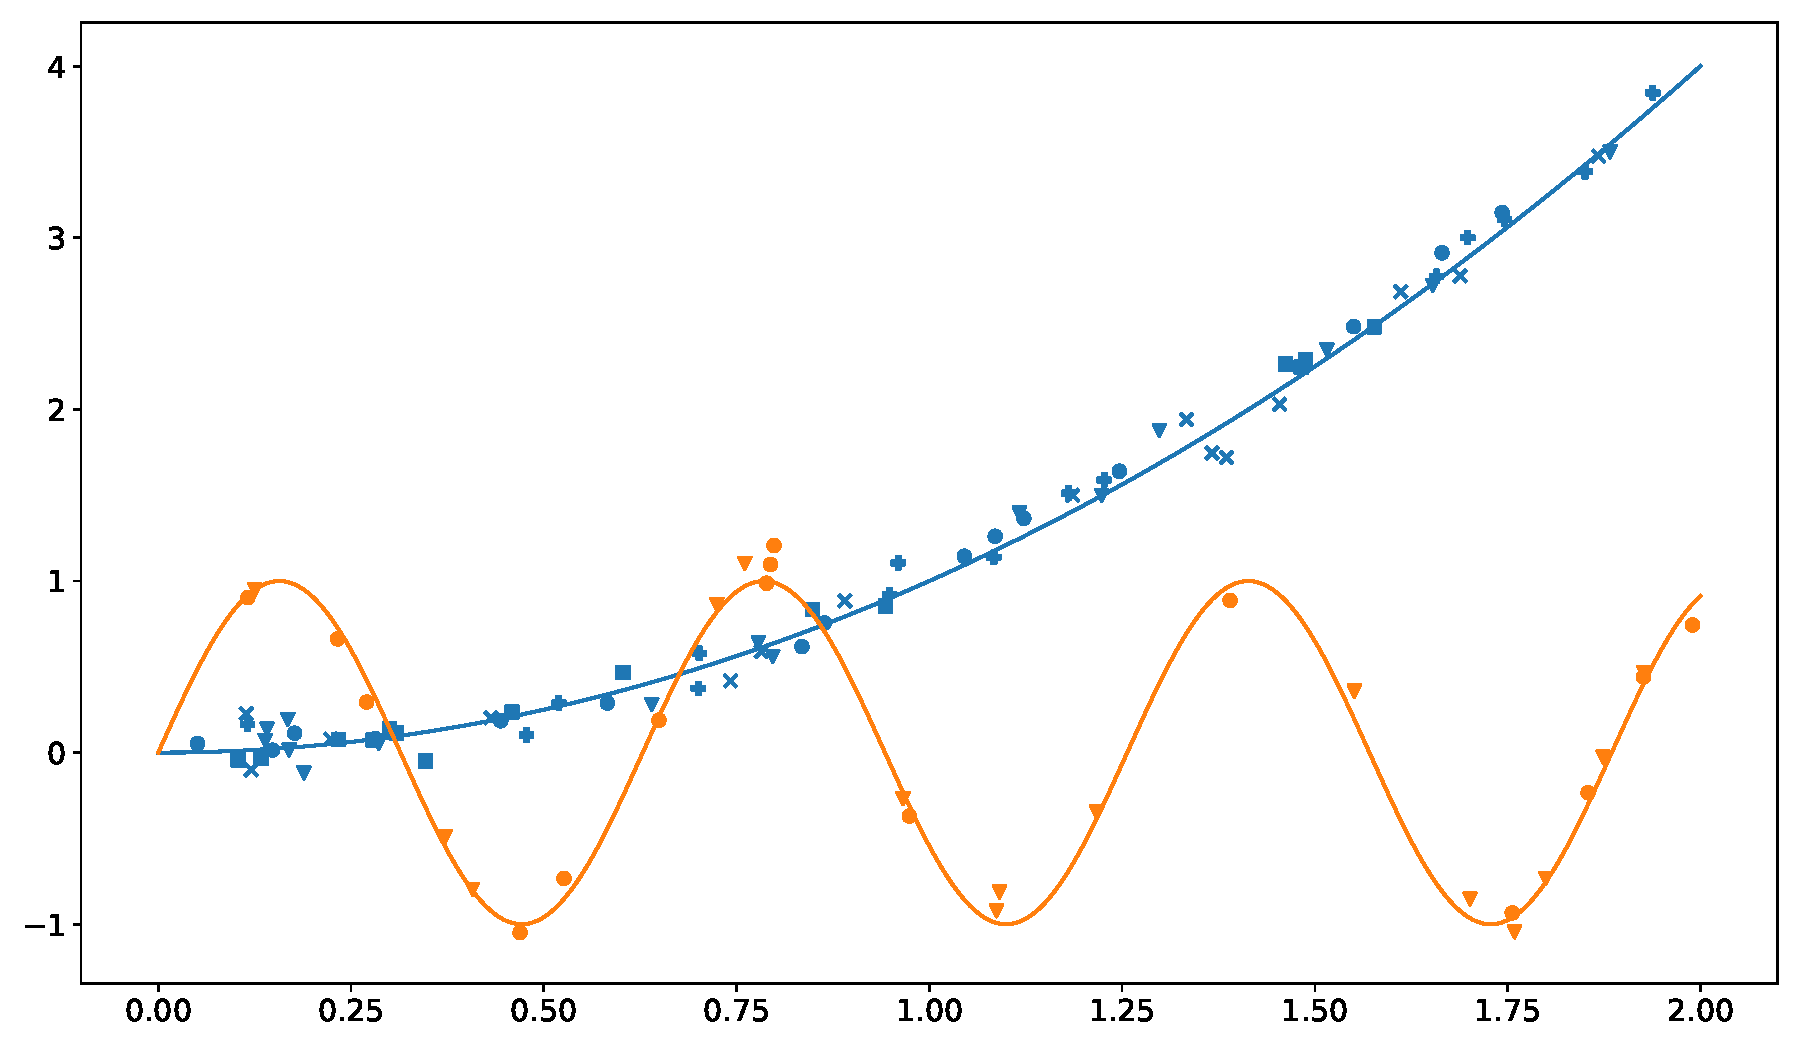
\includegraphics[width=\textwidth]{Chapter6/IGPL2022/regClusters__1.pdf}
%       %       \caption{\fdata{regClusters1}.}
%       %       % \label{regClusters0}
%       % \end{subfigure}
%       % \hfill
%       % \begin{subfigure}[b]{0.49\textwidth}
%       %       \centering
%       %       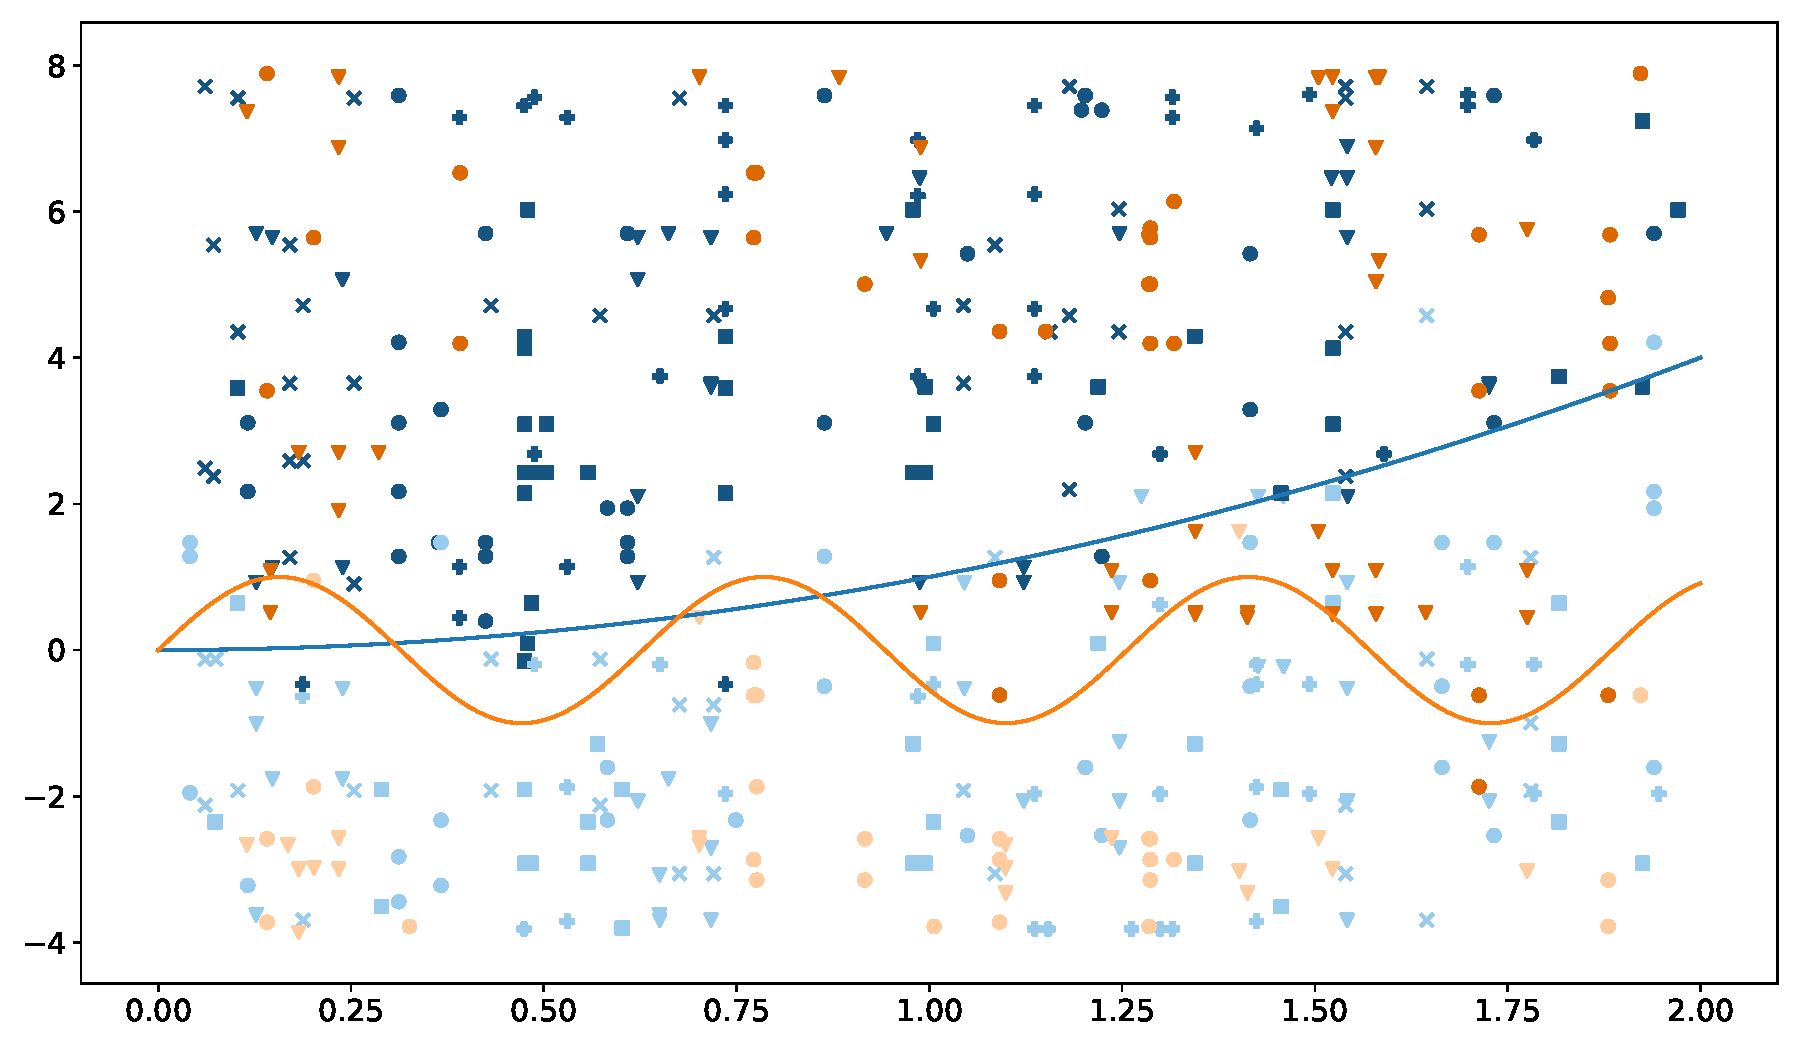
\includegraphics[width=\textwidth]{Chapter6/IGPL2022/clasClusters__1.pdf}
%       %       \caption{\fdata{clasClusters1}.}
%       %       %\label{clasClusters0}
%       % \end{subfigure}
%       % \end{figure}

% \end{frame}

% \begin{frame}
%       \frametitle{Experimentos Sintéticos: Problemas}

%       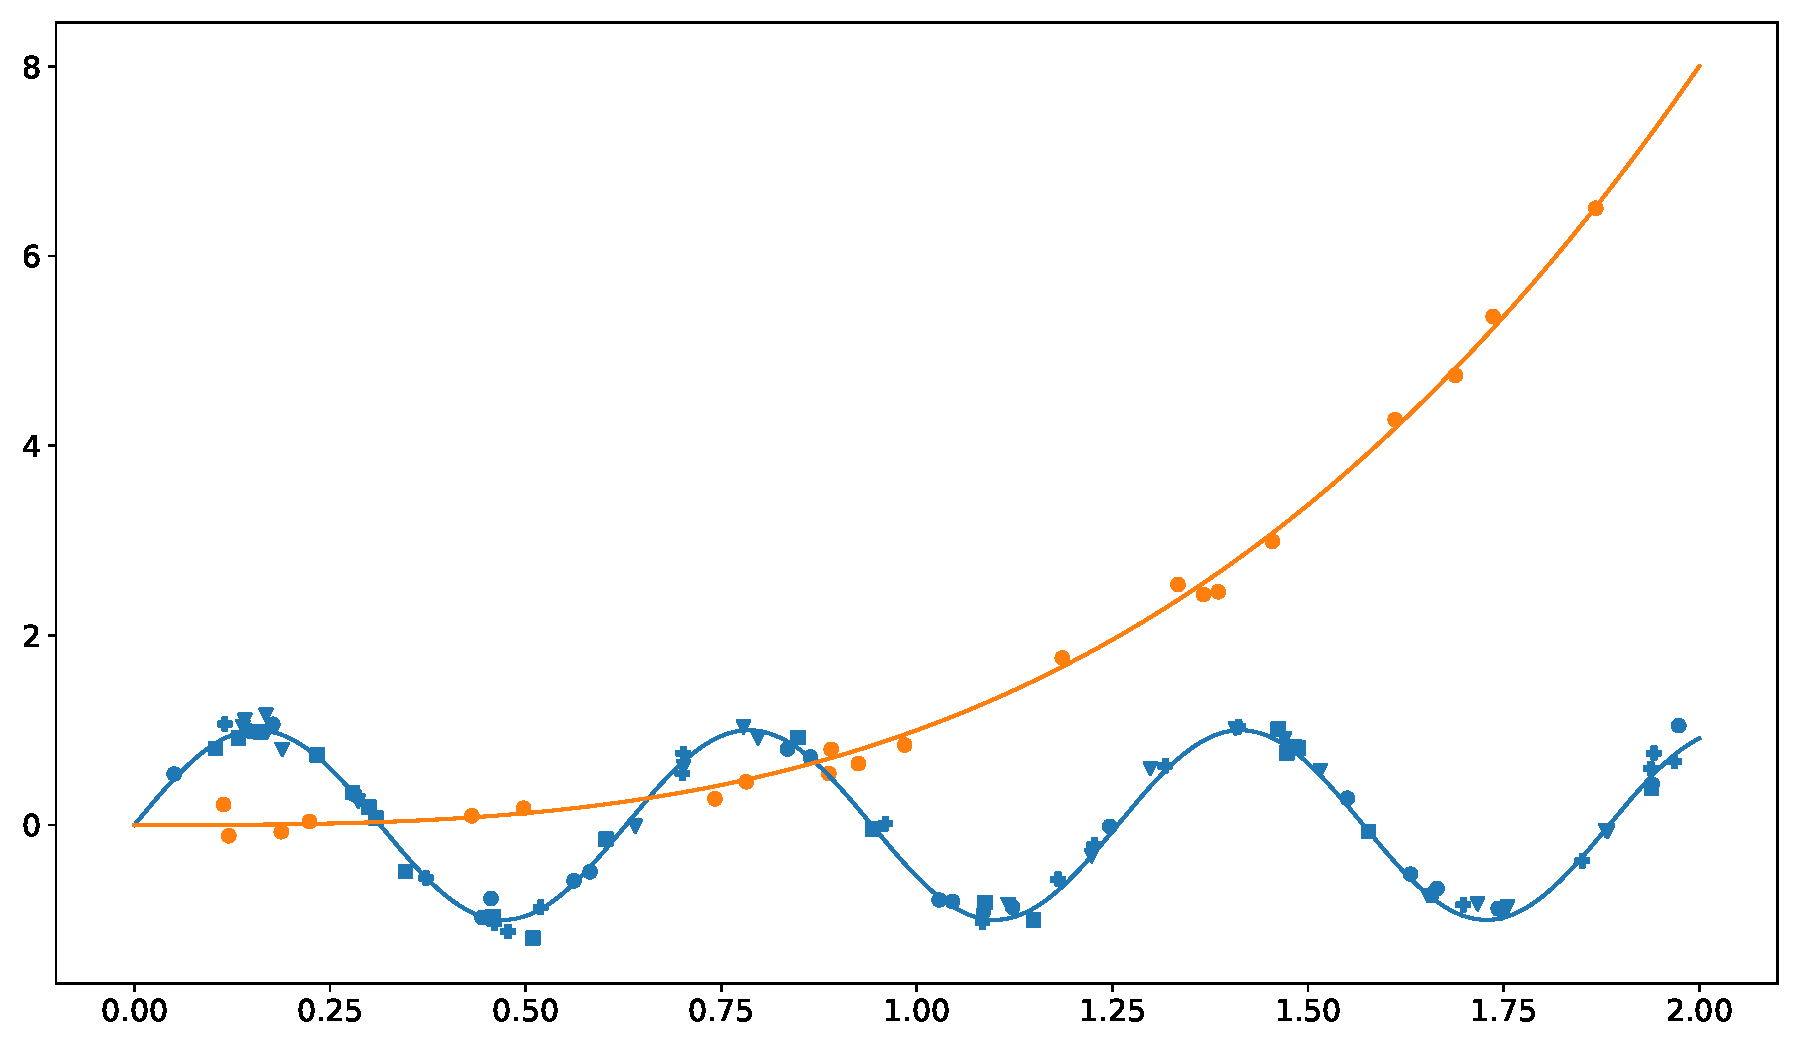
\includegraphics[width=.5\textwidth]{Chapter6/IGPL2022/regClusters__2.pdf}%
%       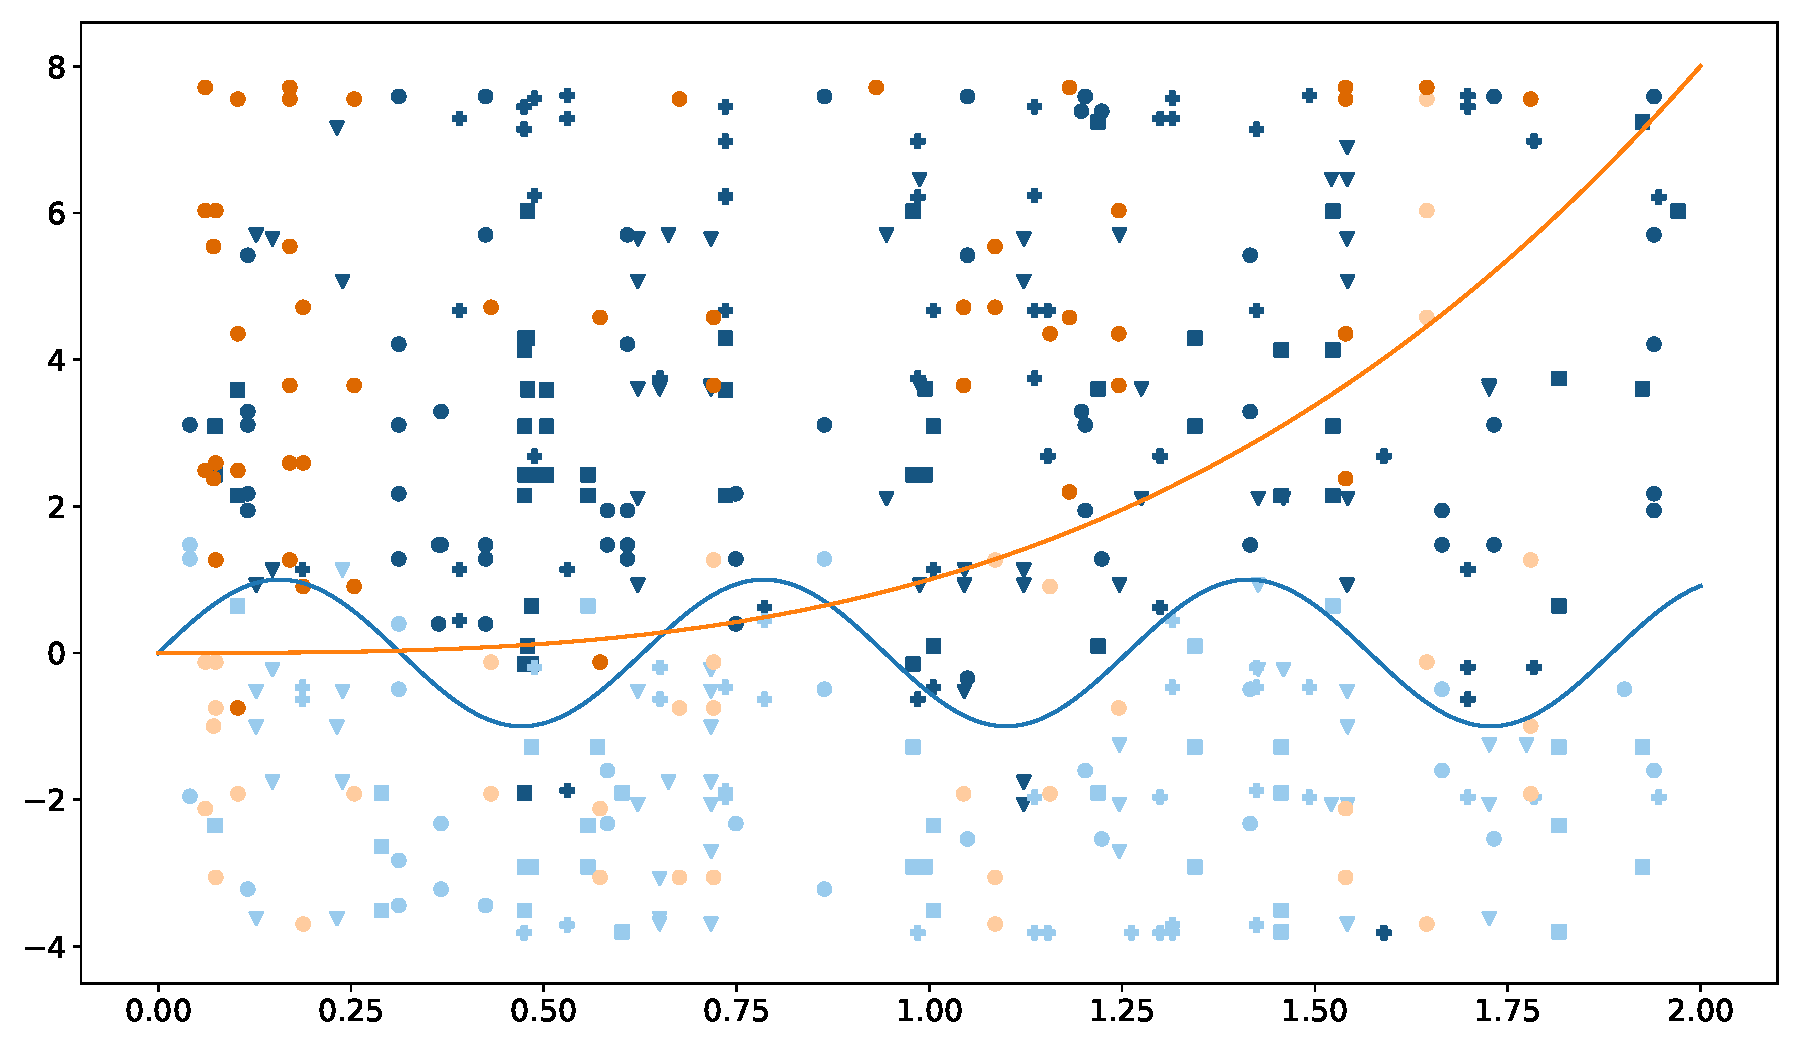
\includegraphics[width=.5\textwidth]{Chapter6/IGPL2022/clasClusters__2.pdf}

%       % \begin{figure}
%       % \begin{subfigure}[b]{0.49\textwidth}
%       %       \centering
%       %       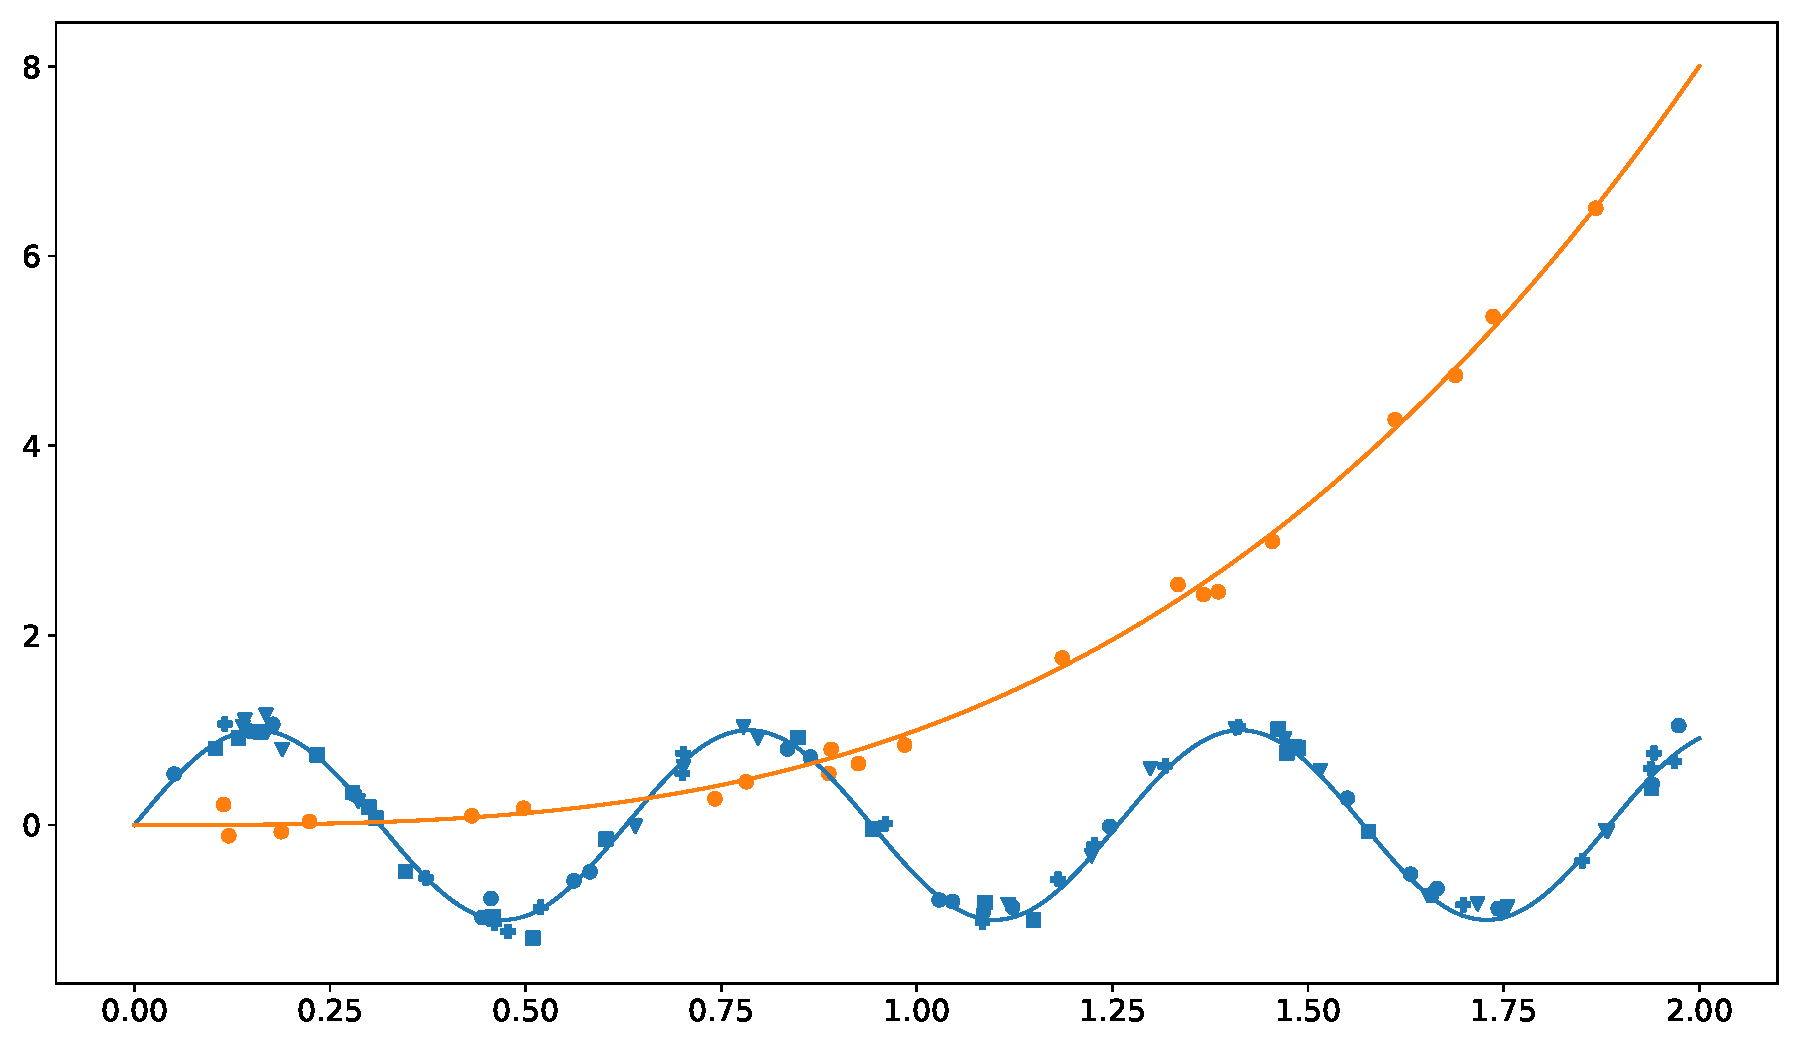
\includegraphics[width=\textwidth]{Chapter6/IGPL2022/regClusters__2.pdf}
%       %       \caption{\fdata{regClusters2}.}
%       %       % \label{regClusters0}
%       % \end{subfigure}
%       % \hfill
%       % \begin{subfigure}[b]{0.49\textwidth}
%       %       \centering
%       %       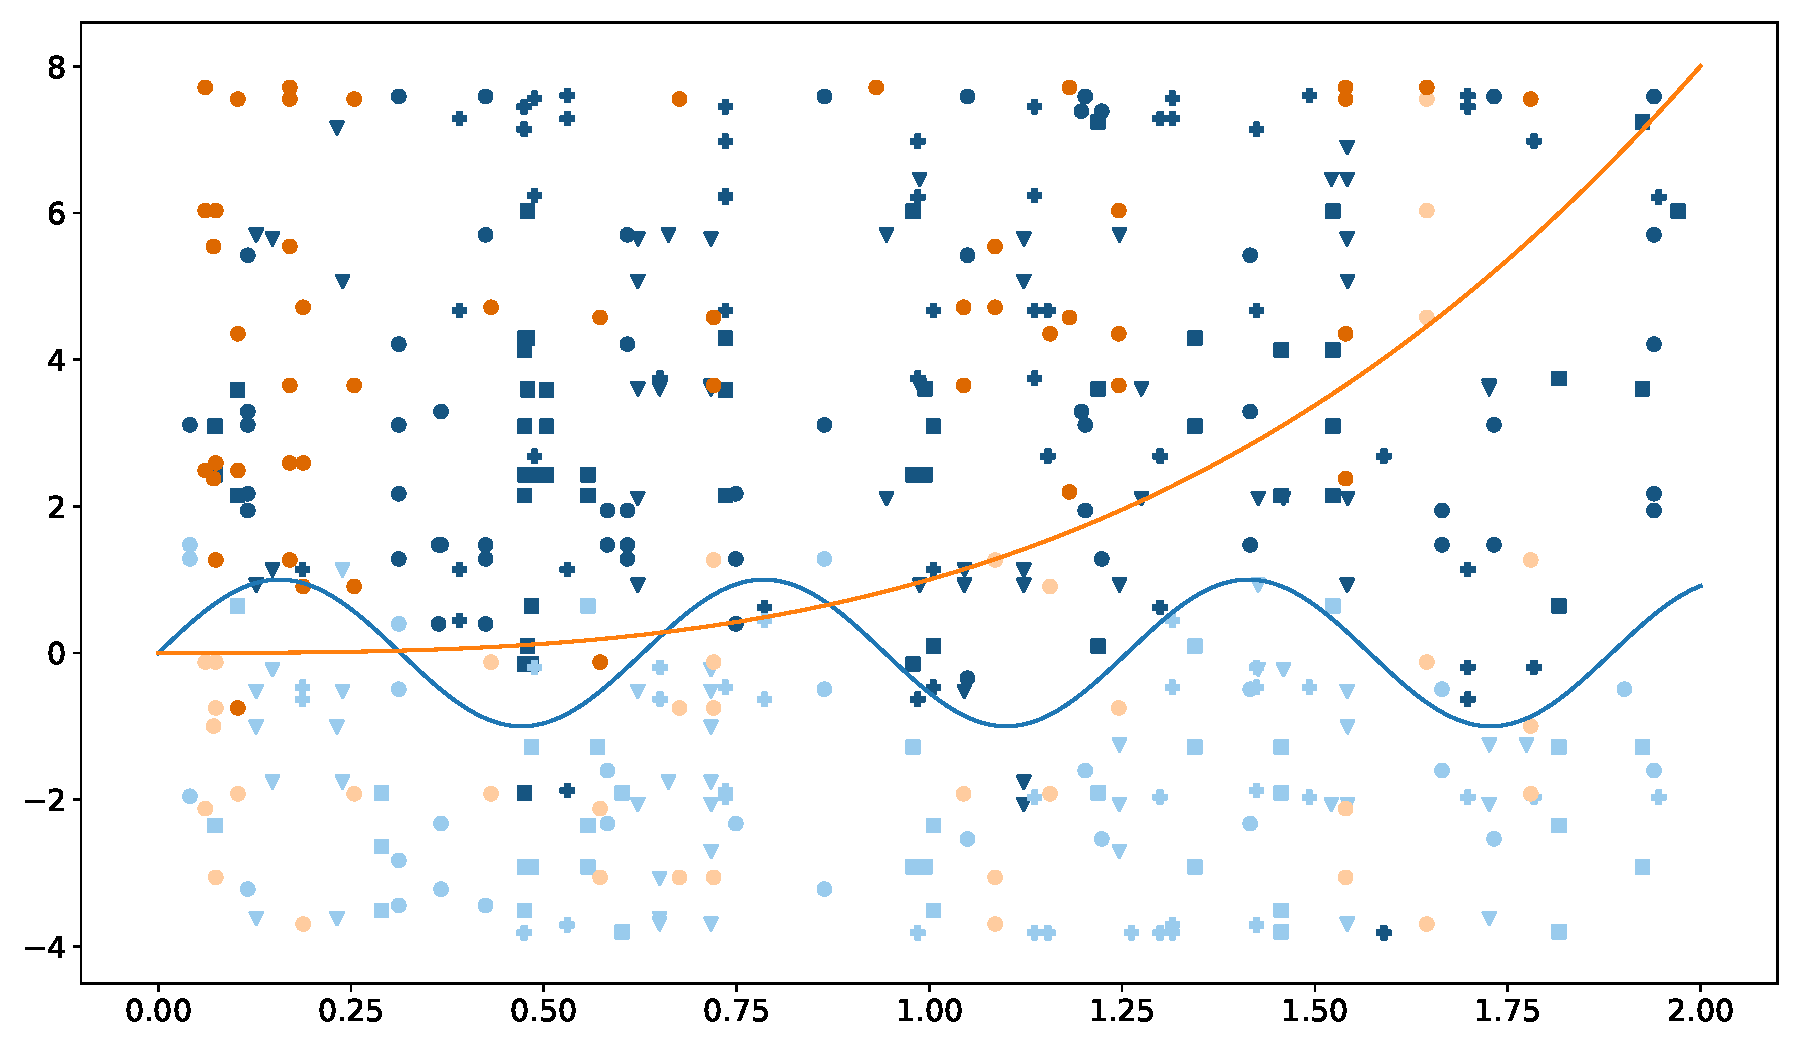
\includegraphics[width=\textwidth]{Chapter6/IGPL2022/clasClusters__2.pdf}
%       %       \caption{\fdata{clasClusters2}.}
%       %       %\label{clasClusters0}
%       % \end{subfigure}
%       % \end{figure}

% \end{frame}



\begin{frame}
      \frametitle{Experimentos Sintéticos: Resultados}

      \begin{table}
            % \caption{\acrshort{mae} scores for synthetic regression problems and F1 scores for synthetic classification ones. In bold we highlight the best models of each group: L1, L2 or LS-\acrshort{svms}.}
            % \label{tab:full_synthetic}
            \centering
            \scalebox{.7}{
            \begin{tabular}{lccc|ccc}
                \toprule
                {} &  \fhead{\fdata{regClusters0}} &  \fhead{\fdata{regClusters1}} &  \fhead{\fdata{regClusters2}} &  \fhead{\fdata{clasClusters0}} &  \fhead{\fdata{clasClusters1}} &  \fhead{\fdata{clasClusters2}} \\
                \midrule
                & \fheadmulti{3}{MAE} & \fheadmulti{3}{F1} \\
                \midrule
                \fmod{CTL-L1}               &            0.989 &            0.512 &            0.541                 &             0.901 &             0.912 &             0.904 \\
                \fmod{ITL-L1}               &            0.221 &            0.212 &            0.159                 &             0.922 &             0.923 &             0.910 \\
                \fmod{MTL-L1}         &            0.213 &            0.176 &            0.135           &             \fmaxn{0.924} &             0.925 &             0.914 \\
                \fmod{cvxGLMTL-L1}       &            0.212 &            0.173 &            0.138         &             0.920 &             0.926 &             0.912 \\
                \fmod{AdapGLMTL-L1}   &            \fmaxn{0.152} &            \fmaxn{0.116} &            \fmaxn{0.107}     &             \fmaxn{0.924} &             \fmaxn{0.929} &             \fmaxn{0.916} \\
                \midrule
                \fmod{CTL-L2}             &            0.990 &            0.642 &            0.768               &             0.904 &             0.912 &             0.906 \\
                \fmod{ITL-L2}             &            0.213 &            0.201 &            0.154               &             \fmaxn{0.928} &             0.928 &             0.910 \\
                \fmod{MTL-L2}       &            0.209 &            0.168 &            0.131         &             0.925 &             0.927 &             0.913 \\
                \fmod{cvxGLMTL-L2}     &            0.204 &            0.169 &            0.131       &             0.921 &             0.923 &             \fmaxn{0.915} \\
                \fmod{AdapGLMTL-L2} &            \fmaxn{0.141} &            \fmaxn{0.115} &            \fmaxn{0.103}   &             0.924 &             \fmaxn{0.929} &             \fmaxn{0.915} \\
                \midrule
                \fmod{CTL-LS}             &            0.989 &            0.642 &            0.766               &             0.895 &             0.908 &             0.894 \\
                \fmod{ITL-LS}             &            0.212 &            0.209 &            0.149               &             0.914 &             0.915 &             0.904 \\
                \fmod{MTL-LS}       &            0.206 &            0.167 &            0.131         &             0.917 &             0.917 &             \fmaxn{0.905} \\
                \fmod{cvxGLMTL-LS}     &            0.207 &            0.169 &            0.132       &             0.919 &             \fmaxn{0.921} &             0.897 \\
                \fmod{AdapGLMTL-LS} &            \fmaxn{0.136} &            \fmaxn{0.115} &            \fmaxn{0.106}   &             \fmaxn{0.920} &             \fmaxn{0.921} &             0.901 \\
                \bottomrule
            \end{tabular}
            }
        \end{table}

\end{frame}

\begin{frame}
      \frametitle{Experimentos Sintéticos: Matrices de Adyacencia}
      
      \centering
      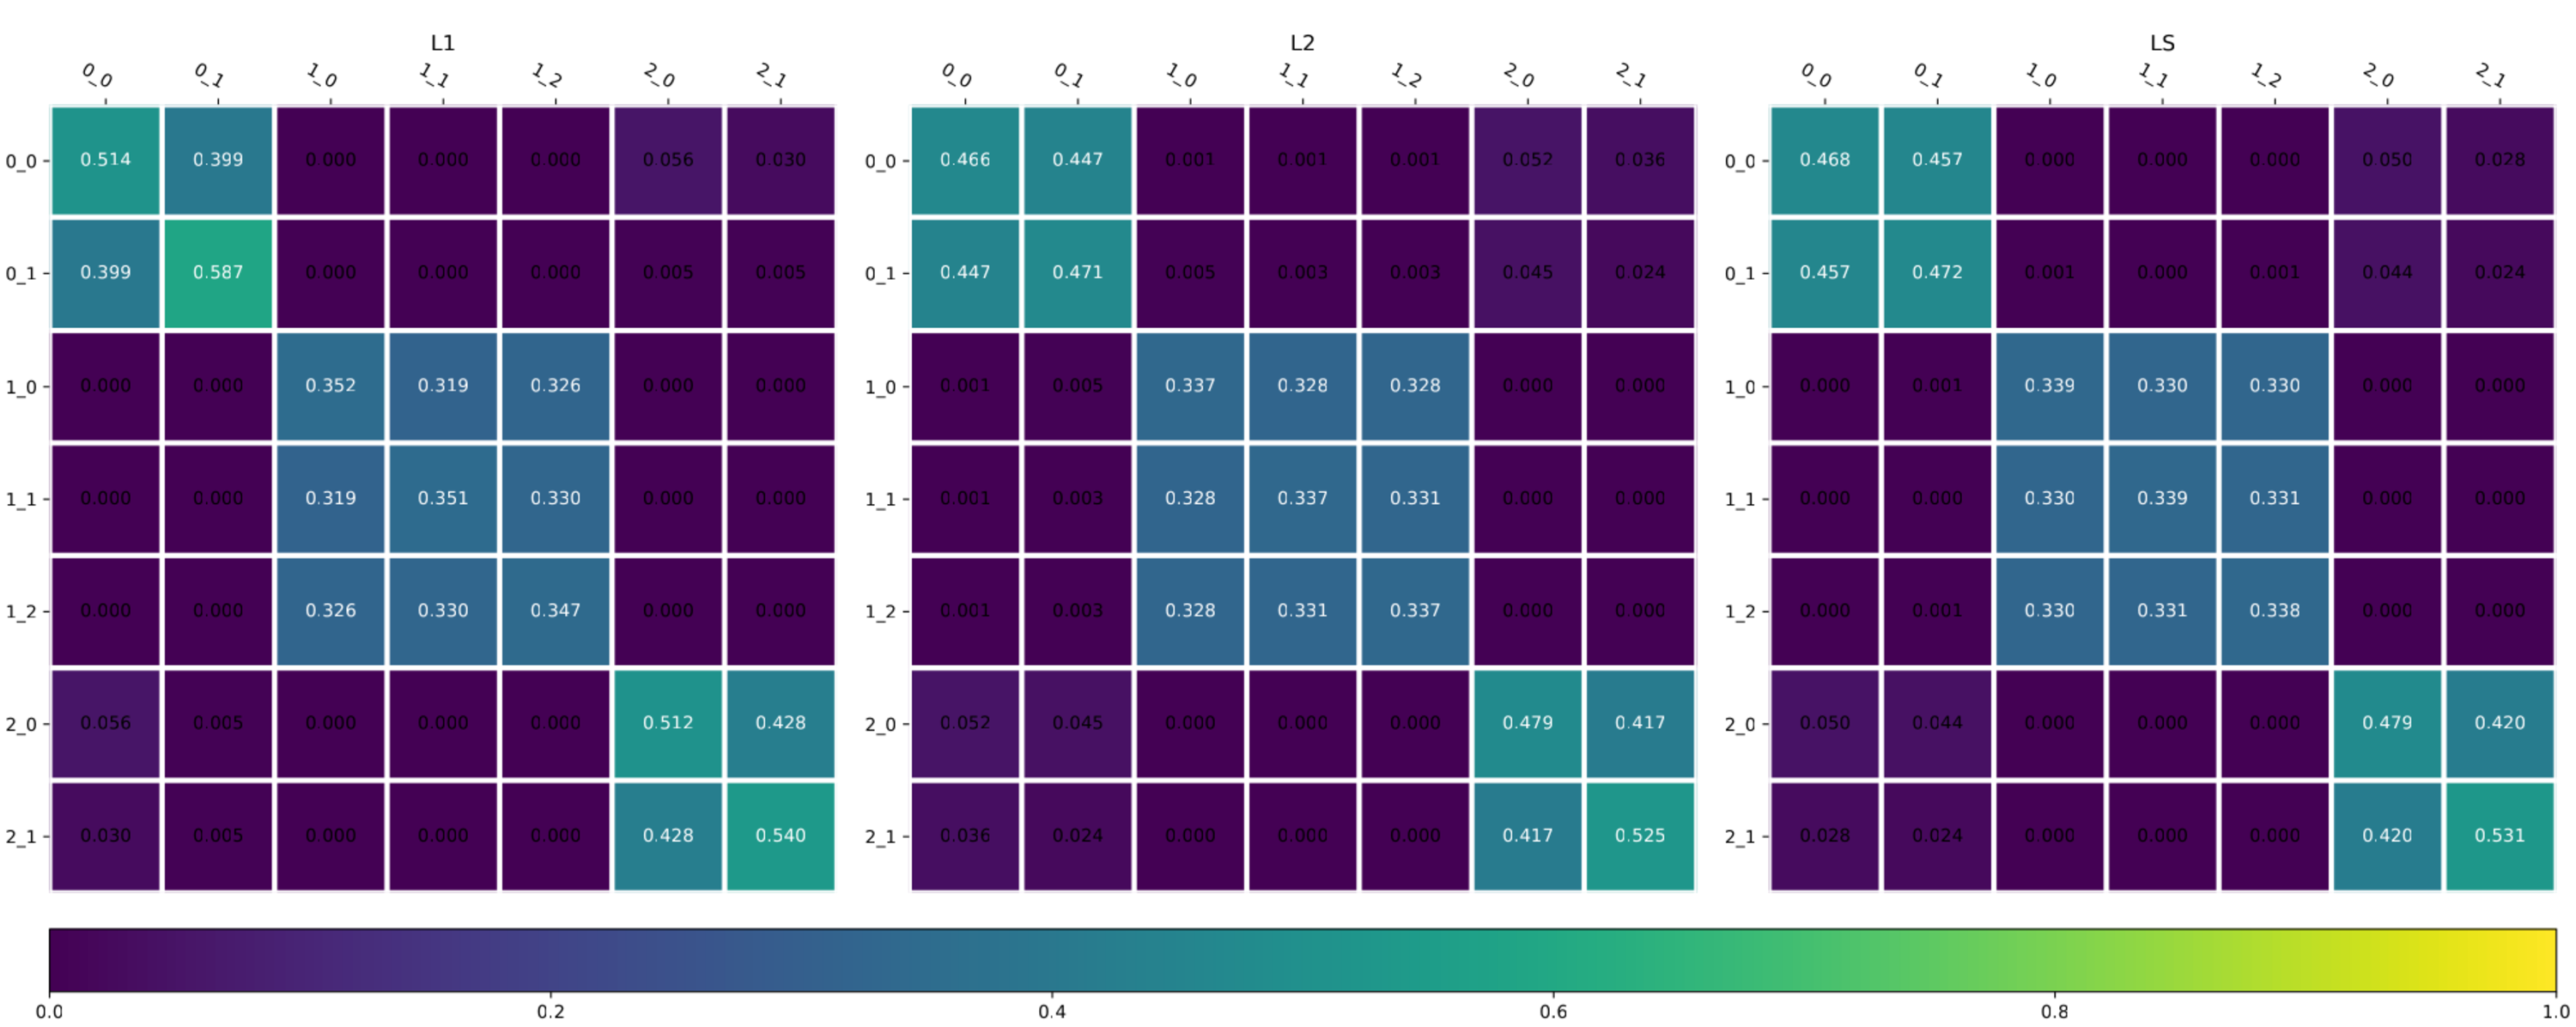
\includegraphics[width=.95\textwidth]{Chapter6/IGPL2022/adjMatrix_all__regClusters_0_crop.pdf}

      \begin{itemize}
            \item Matrices de \fdata{regClusters0} para L1, L2 y LS-SVM MT de laplaciano adaptativo
      \end{itemize}
      
      % \begin{figure}
      %       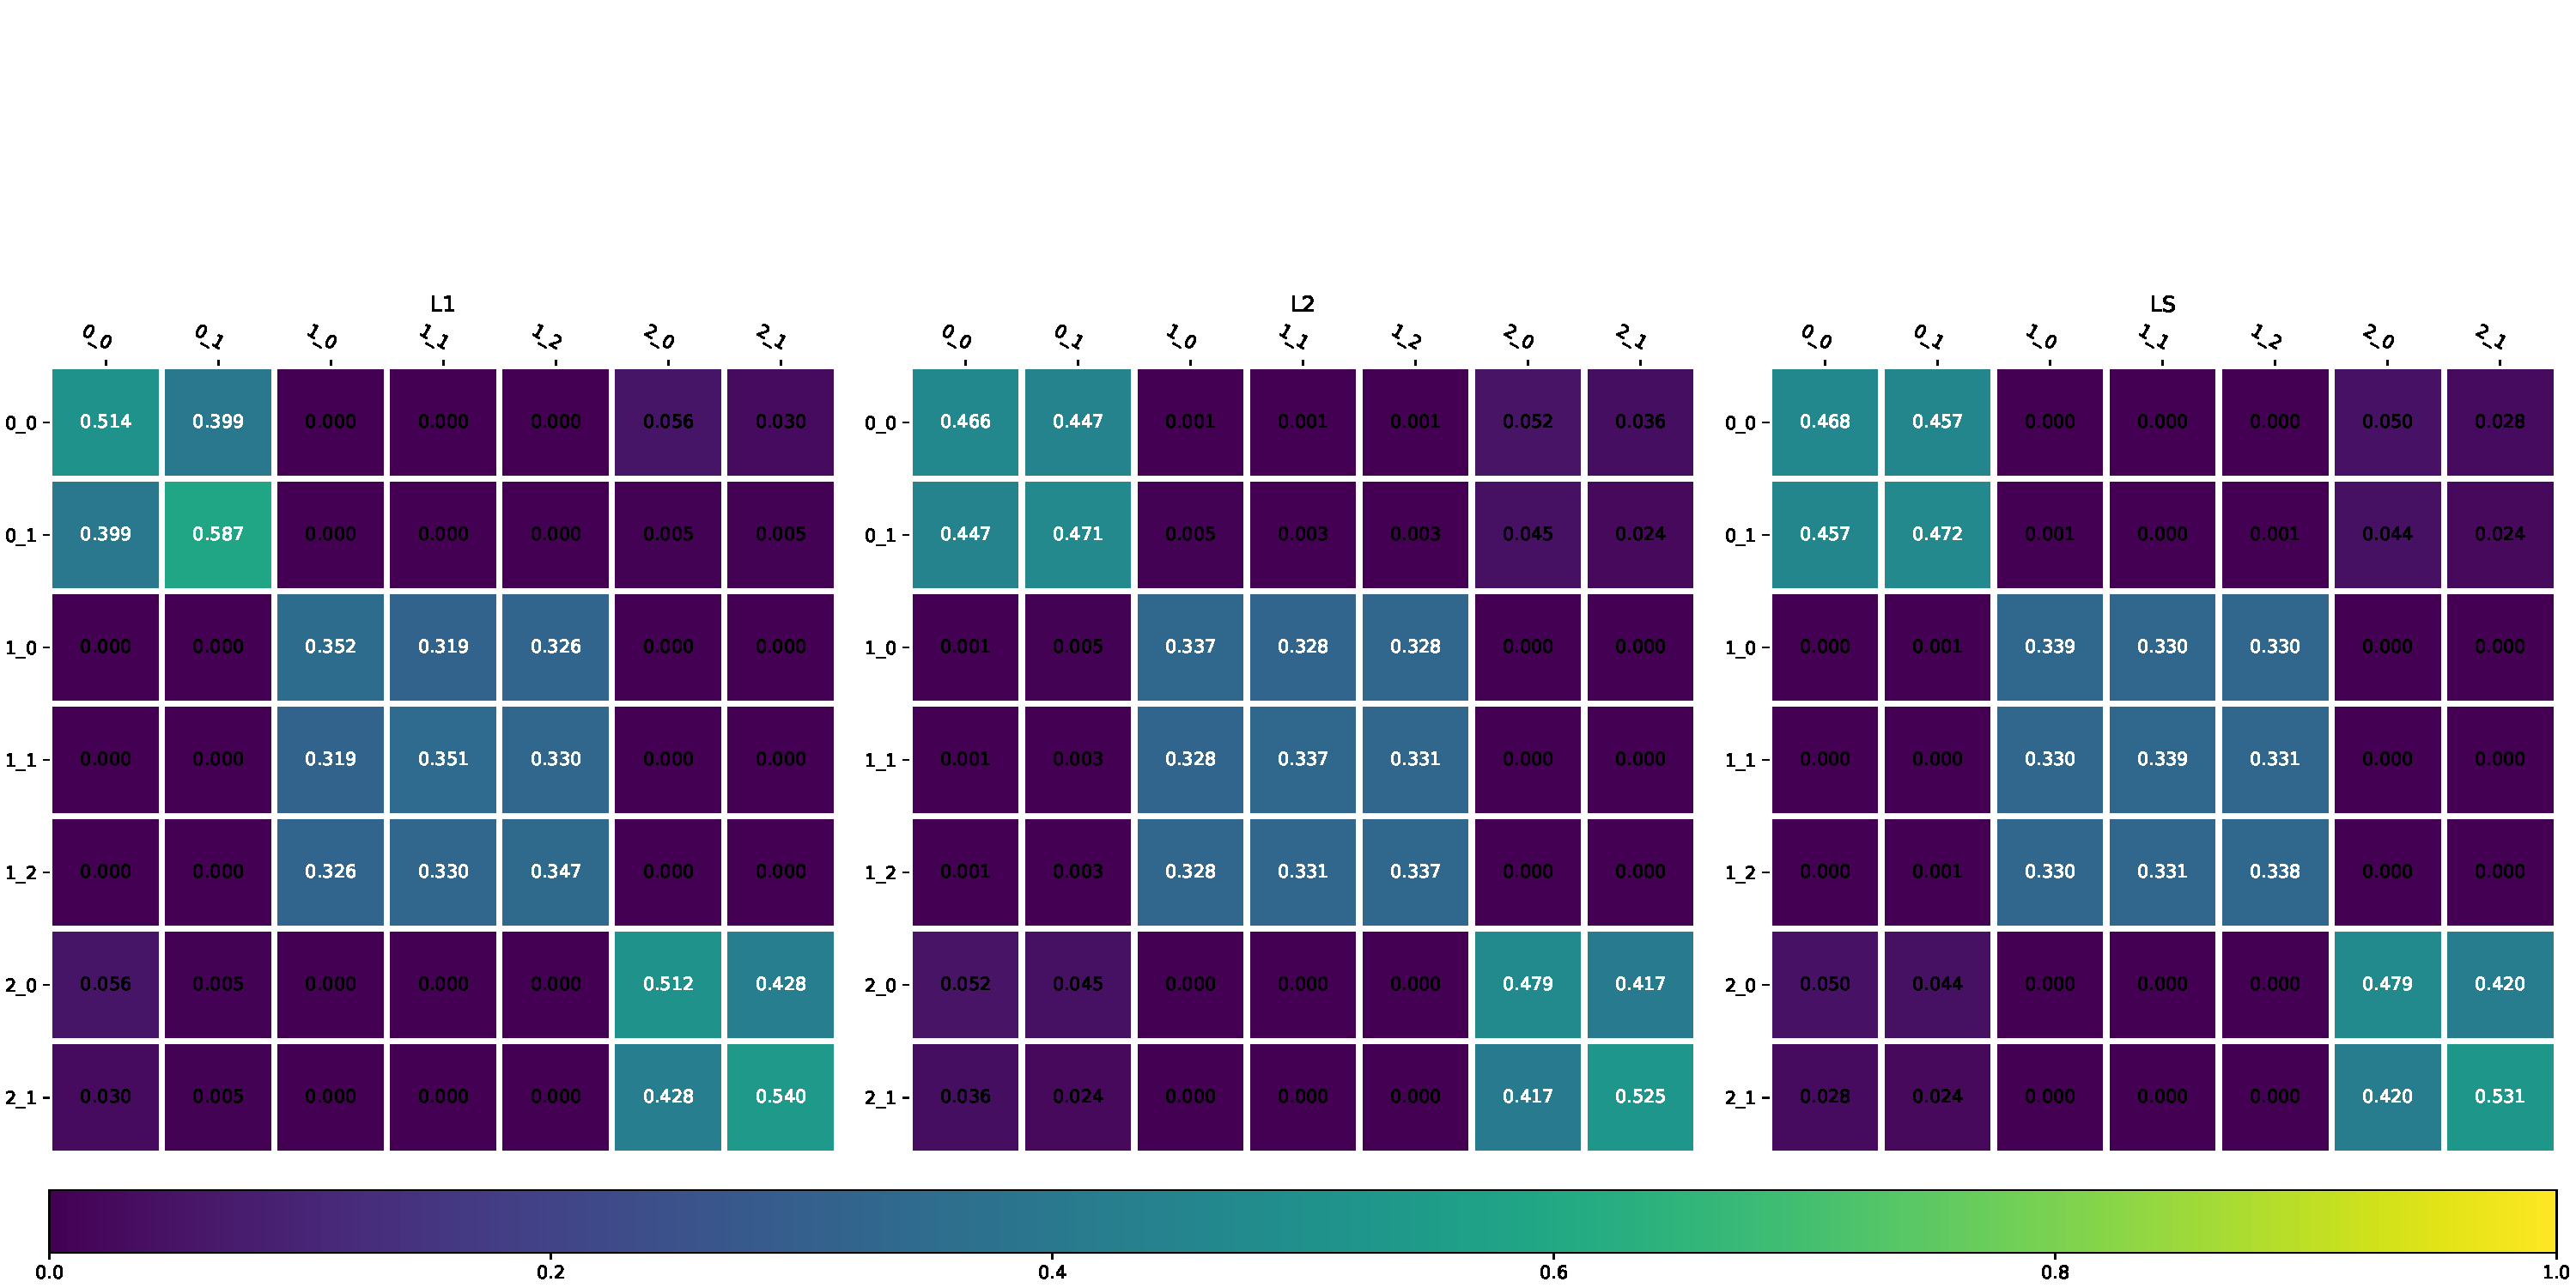
\includegraphics[width=.95\textwidth]{Chapter6/IGPL2022/adjMatrix_all__regClusters_0.pdf}
      %       \caption{Matrices de \fdata{regClusters0} para L1, L2 y LS-SVM MT de laplaciano adaptativo.}
      % \end{figure}

\end{frame}

\begin{frame}
      \frametitle{Experimentos Sintéticos: Matrices de Adyacencia}
      \centering
      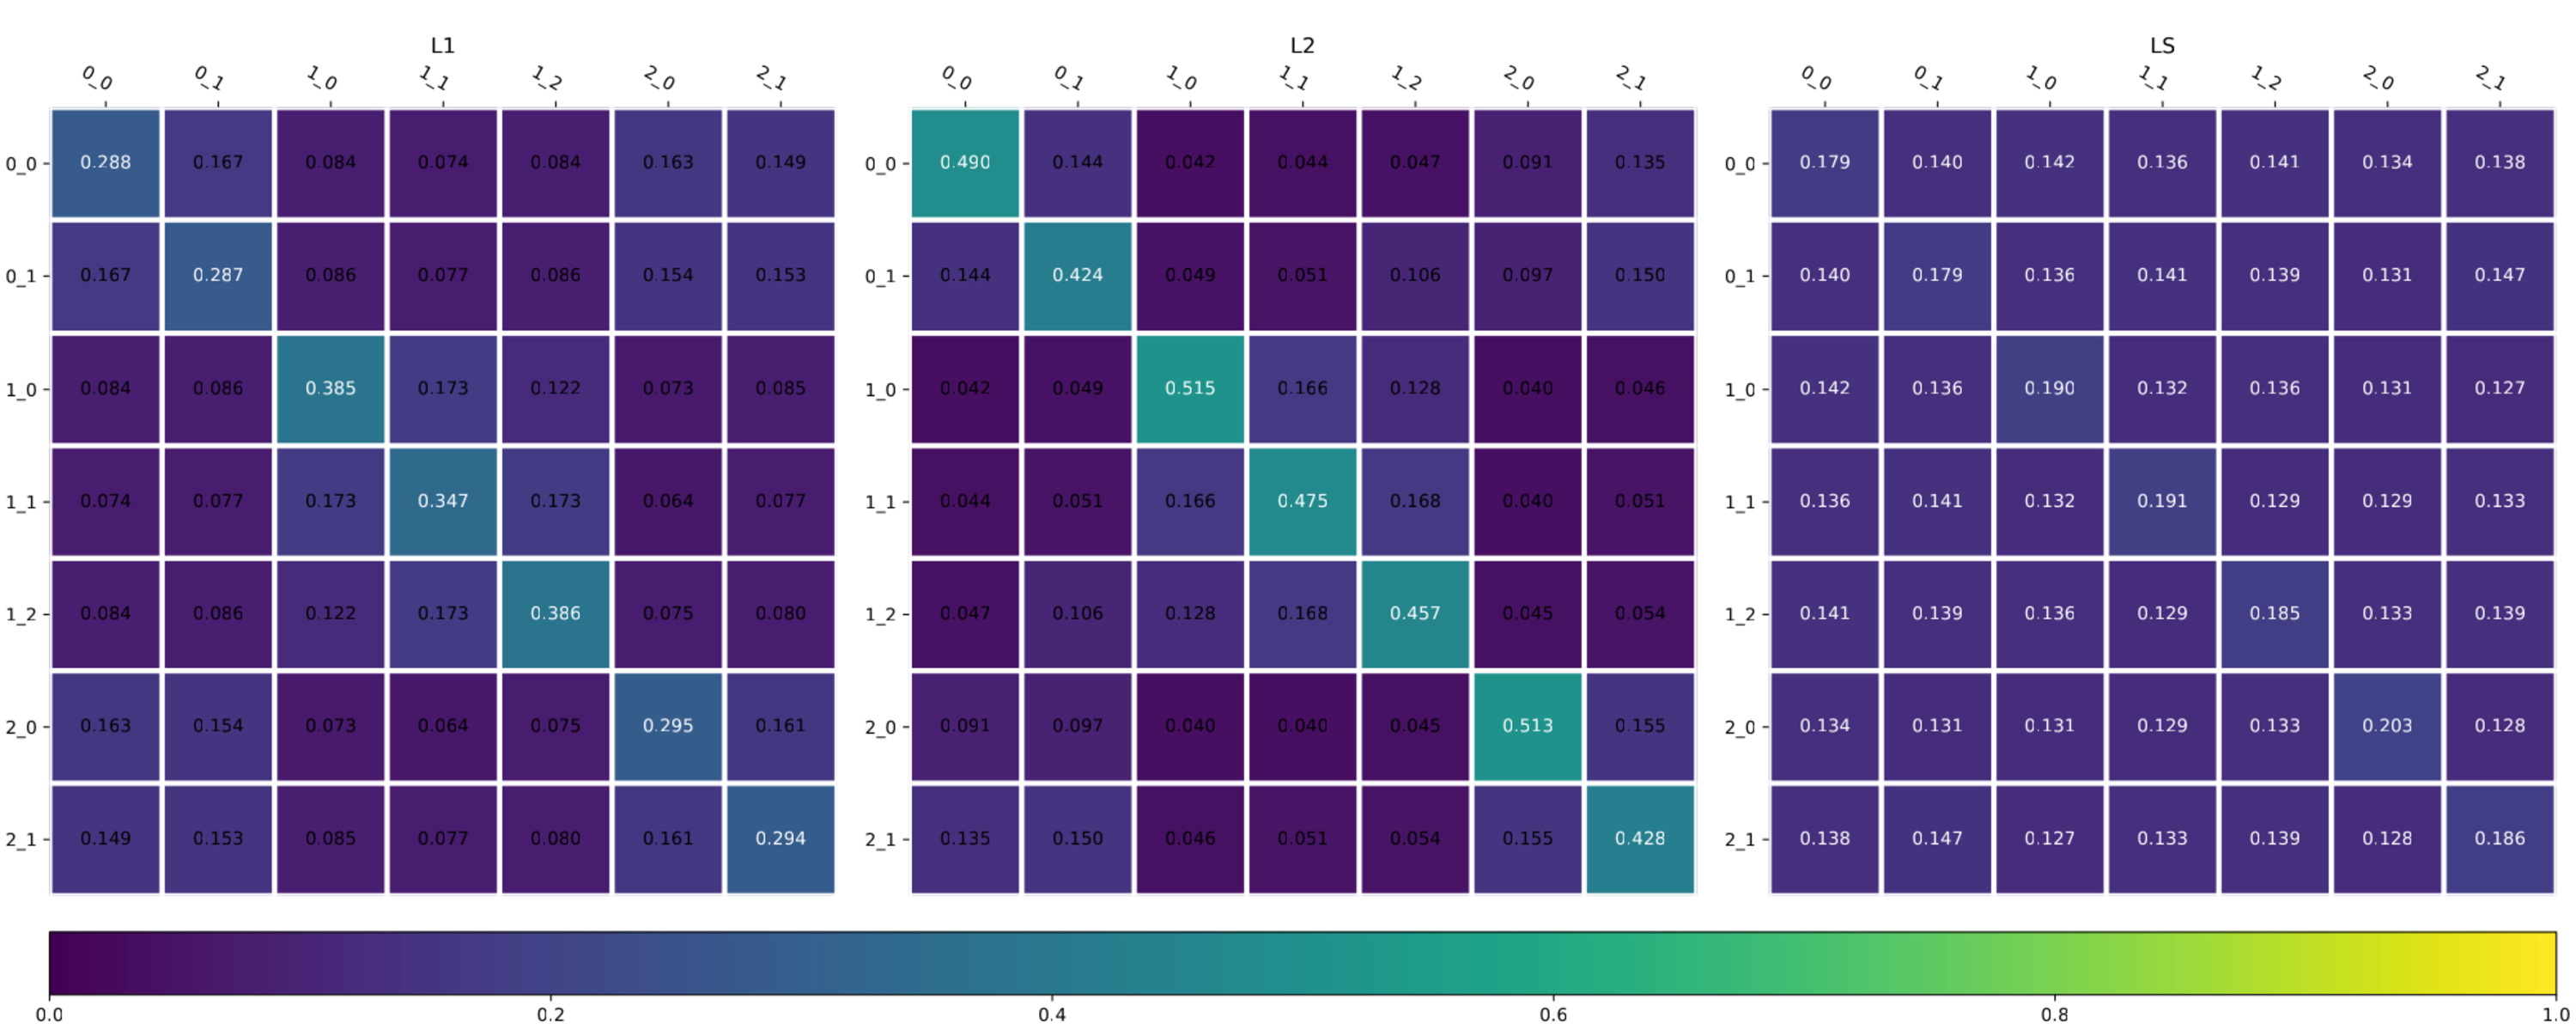
\includegraphics[width=.95\textwidth]{Chapter6/IGPL2022/adjMatrix_all__clasClusters_0_crop.pdf}

      \begin{itemize}
            \item Matrices de \fdata{clasClusters0} para L1, L2 y LS-SVM MT de laplaciano adaptativo
      \end{itemize}      
      % \centering
      % \begin{figure}
      %       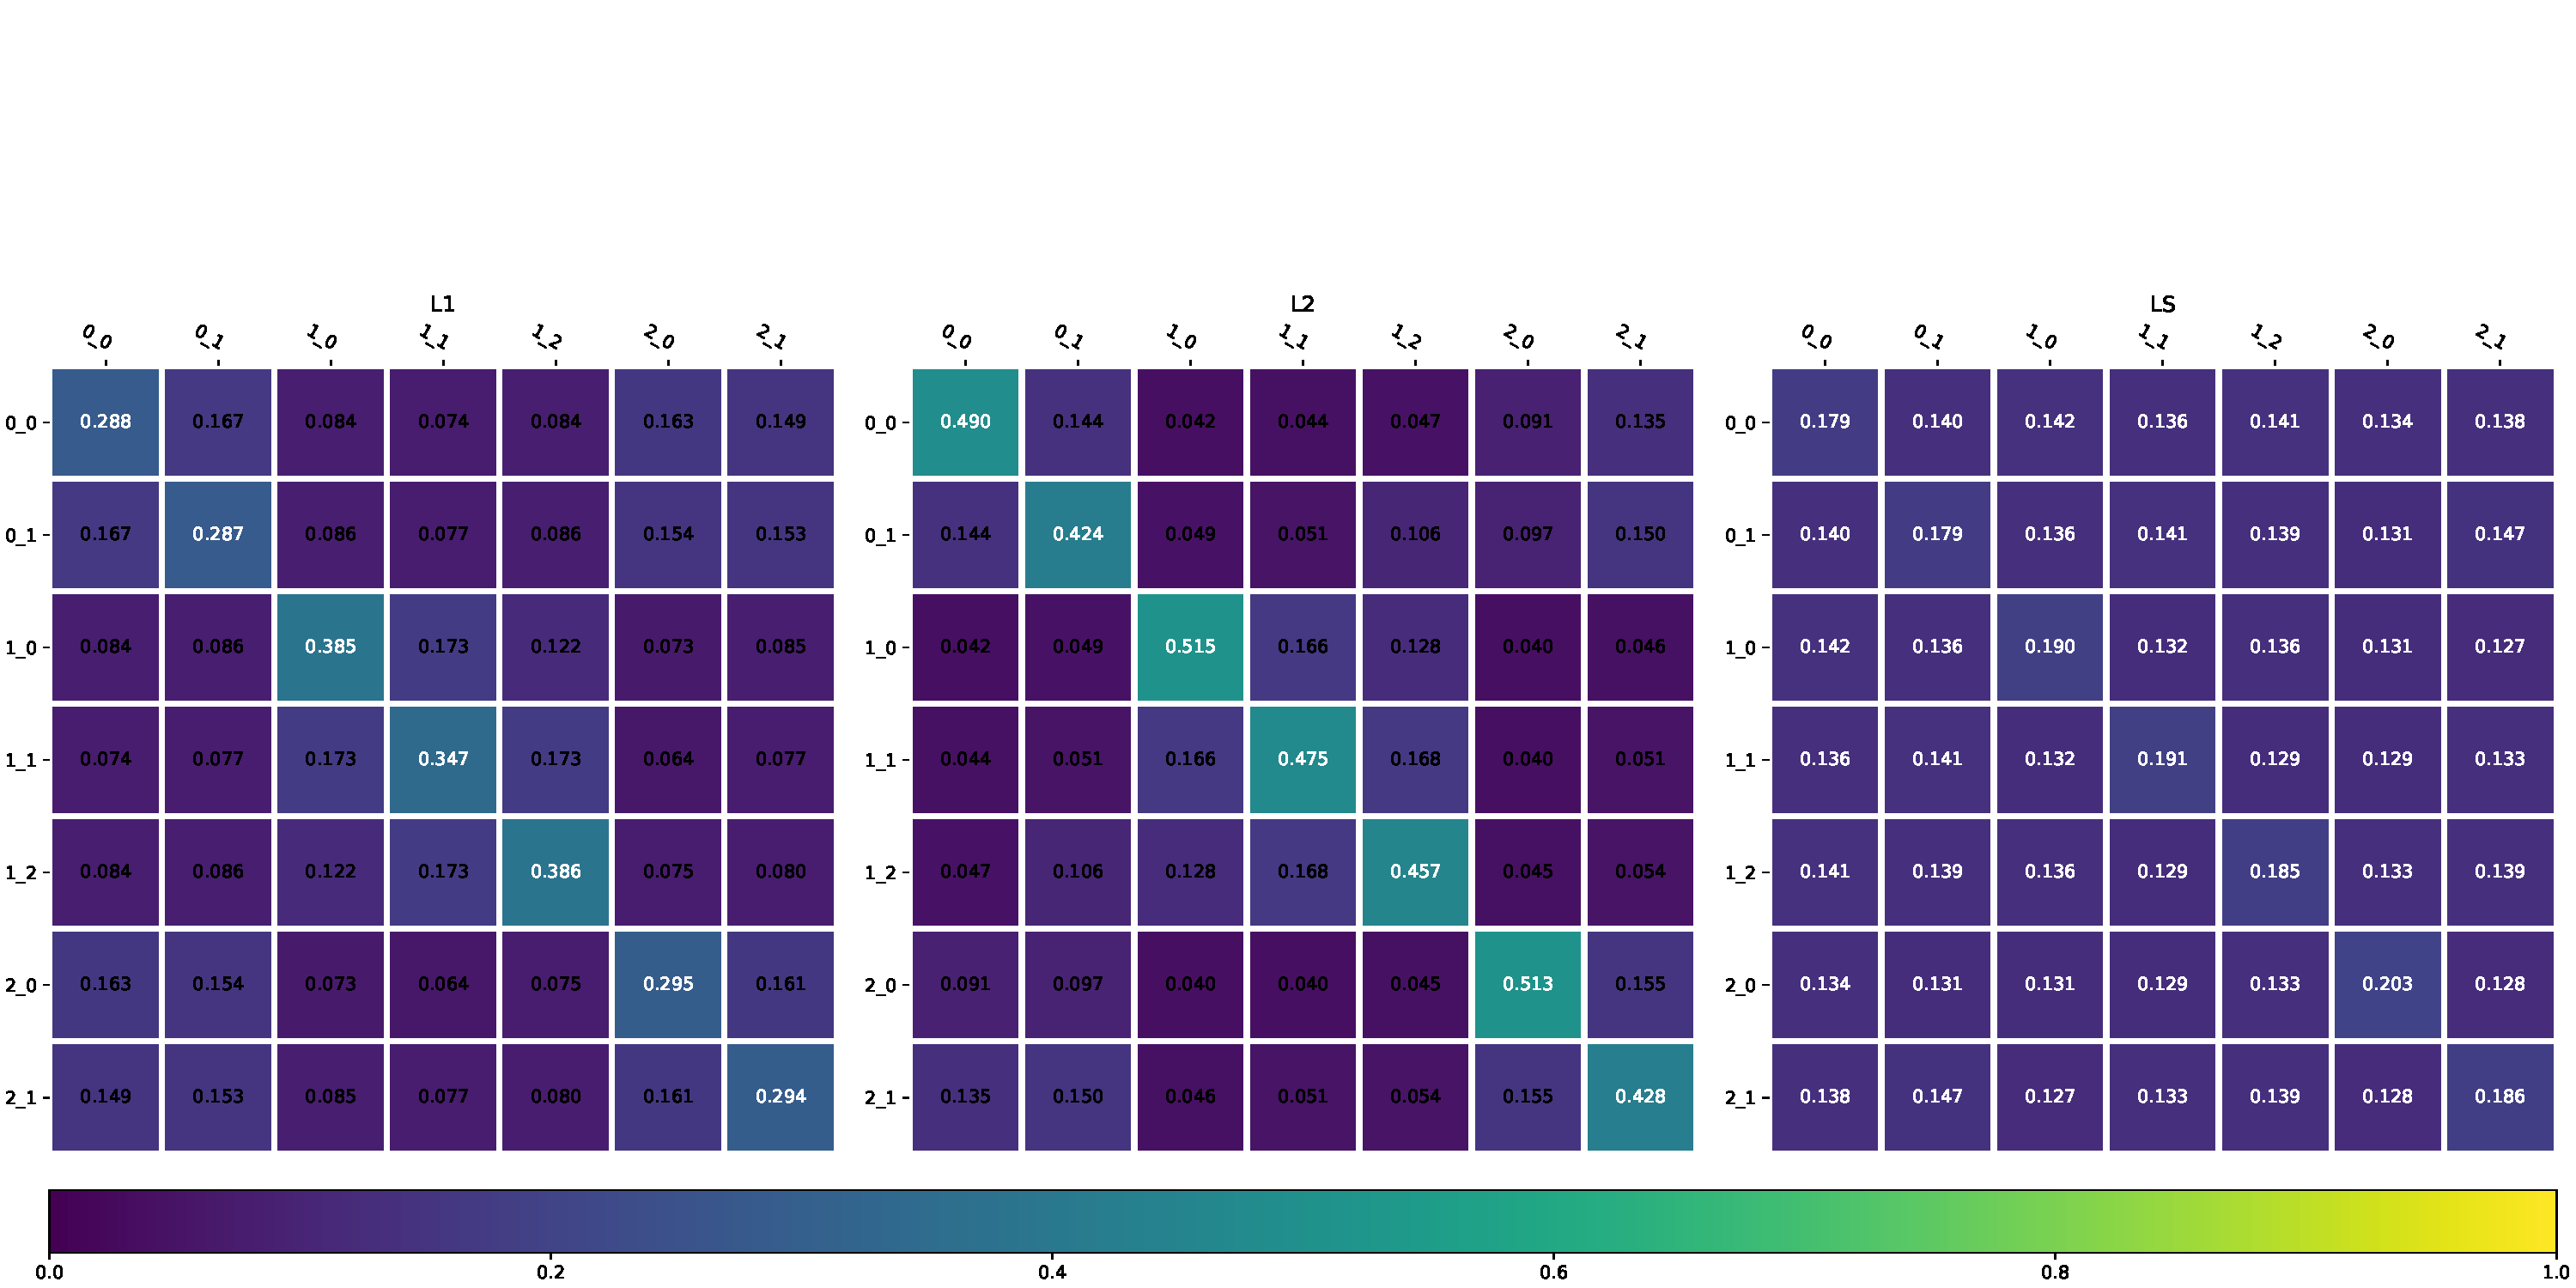
\includegraphics[width=.95\textwidth]{Chapter6/IGPL2022/adjMatrix_all__clasClusters_0.pdf}
      %       \caption{Matrices de \fdata{clasClusters0} para L1, L2 y LS-SVM MT de laplaciano adaptativo.}
      % \end{figure}

\end{frame}


% \begin{frame}
%       \frametitle{Experimentos Reales: Procedimiento}

      
%       \centering
%             \scalebox{.7}{
%             \begin{tabular}{*{7}{c}}
%             \toprule
%             \fhead{} & \fhead{Grid} & \fhead{\fmod{CTL}} & \fhead{\fmod{ITL}} & \fhead{\fmod{MTL}} & \fhead{\fmod{GLMTL}} & \fhead{\fmod{cvxGLMTL}} \\
%              \midrule
%             $C$ &  \scalebox{1}{$\set{4^k: -2 \leq k \leq 2}$} & CV & CV & CV & CV & CV  \\ 
%             $\epsilon$ & \scalebox{1}{$\set{\frac{\sigma}{4^k}: 1 \leq k \leq 6}$} & CV & CV & CV & CV & CV  \\
%             $\gamma$ & \scalebox{1}{$\set{\frac{4^k}{d}: -2 \leq k \leq 3}$} & CV & - & \fmod{CTL} & - & \fmod{CTL} \\
%             $\gamma_s$ & \scalebox{1}{$\set{\frac{4^k}{d}: -2 \leq k \leq 3}$} & - & CV & \fmod{ITL} & \fmod{CTL} & \fmod{CTL}\\
%             $\lambda$ & \scalebox{1}{$\set{0.2 k : 0 \leq k \leq 5}$} & - & - & CV & - & CV\\
%             $\mu$ & \scalebox{1}{$\set{4^k : -1 \leq k \leq 3}$} & - & - & - & CV & \fmod{GLMTL}\\
%             \bottomrule
%             \end{tabular}
%             }
%       \vfill
%       \begin{itemize}
%             \item Usamos 5 particiones externas y obtenemos 5 scores de test
%             \item Usamos la Validación Cruzada (CV) con 5 particiones internas para la búsqueda en rejilla de los hiperparámetros
%       \end{itemize}

% \end{frame}


% \begin{frame}
%       \frametitle{Experimentos Reales: Resultados}

%       %\begin{table*}[H]
%             % \caption{Test results for real problems.
%             % We show the average and standard deviation of MAE scores for the regression problems: \fdata{computer} and \fdata{parkinson}; and average and standard deviation of F1 scores for the classification problem: \fdata{landmine}.
%             % In bold we highlight the best models of each group: L1, L2 or LS-SVMs.}
%             % \label{tab:results_real}
%             \centering
%             \scalebox{.7}{
%             \begin{tabular}{l*{2}{S[table-format=1.3]@{$\pm$}S[table-format=1.3]}|S[table-format=1.3]@{$\pm$}S[table-format=1.3]}
%             \toprule
%             &  \fheadmulti{2}{\fdata{computer}} & \fheadmulti{2}{\fdata{parkinson}} & \fheadmulti{2}{\fdata{landmine}} \\
%             \midrule
%             \fmod{CTL-L1}    & 1.985 & 0.039  & 4.306 & 0.209 & 0.202 & 0.047 \\
%              \fmod{ITL-L1}    & 1.623 & 0.028  & 1.949 & 0.021 & 0.243 & 0.014 \\
%              \fmod{MTL-L1} & \fmaxn{1.526} & \fmaxn{0.052}  & \fmaxn{1.942} & \fmaxn{0.019} & 0.266 & 0.022 \\
%              \fmod{cvxGLMTL-L1}     & \fmaxn{1.526} & \fmaxn{0.052}  & 1.945 & 0.024 & 0.249 & 0.039 \\
%              \fmod{AdapGLMTL-L1} & 1.545 & 0.083  & 1.945 & 0.024 & \fmaxn{0.272} & \fmaxn{0.033} \\
%             \hline
%             \fmod{CTL-L2}    & 2.001 & 0.028 & 4.211 & 0.093 & 0.235 & 0.045 \\
%             \fmod{ITL-L2}    & 2.105 & 0.070 & 1.936 & 0.026 & \fmaxn{0.267} & \fmaxn{0.019} \\
%             \fmod{MTL-L2} & 1.506 & 0.043 & 1.928 & 0.037 & 0.260 & 0.041 \\
%             \fmod{cvxGLMTL-L2}     & 1.507 & 0.045 & \fmaxn{1.927} & \fmaxn{0.037} & 0.251 & 0.048 \\
%             \fmod{AdapGLMTL-L2} & \fmaxn{1.501} & \fmaxn{0.047} & 1.928 & 0.038 & 0.249 & 0.055 \\
%            \hline
%             \fmod{CTL-LS}    & 2.002 & 0.029 & 4.217 & 0.108 & 0.186 & 0.040 \\
%             \fmod{ITL-LS}    & 1.609 & 0.015 & 1.928 & 0.017 & 0.182 & 0.007 \\
%             \fmod{MTL-LS} & 1.507 & 0.042 & 1.929 & 0.026 & 0.186 & 0.041 \\
%             \fmod{cvxGLMTL-LS}     & \fmaxn{1.502} & \fmaxn{0.047} & \fmaxn{1.917} & \fmaxn{0.022} & \fmaxn{0.197} & \fmaxn{0.033} \\
%             \fmod{AdapGLMTL-LS} & 1.506 & 0.046 & 1.924 & 0.033 & 0.196 & 0.031    \\
%                 \bottomrule
%       \end{tabular}}
%         %\end{table*}

% \end{frame}


\section{Conclusiones y Trabajo Futuro}

\begin{frame}
\frametitle{Conclusiones}
\begin{itemize}
      \item El Aprendizaje Multitarea ofrece una serie de ventajas, pero es necesario desarrollar técnicas para crear un acoplamiento de los modelos de cada tarea
      \item Proponemos una formulación que considera la combinación convexa de una parte común a todas las tareas y otra específica
      \item Formulación convexa con métodos de kernel:
      \begin{itemize}
            \item Definimos las L1, L2 y LS-SVM MT con esta formulación convexa 
            \item Analizamos la alternativa que consiste en la combinación convexa de modelos preentrenados
            \item Mostramos buenos resultados de las SVM MT convexas con varios problemas
      \end{itemize}
      \item Formulación convexa con redes neuronales:
      \begin{itemize}
            \item Aplicamos esta formulación convexa también a redes neuronales
            \item Mostramos que nuestra propuesta obtiene mejores resultados que el \emph{Hard Sharing} en cuatro conjuntos de imágenes
      \end{itemize}
            
\end{itemize}
\end{frame}

\begin{frame}
\frametitle{Conclusiones}
\begin{itemize}
      
      \item La formulación convexa asume que todas las tareas comparten una parte común
      \item Las tareas a veces están repetidas o no todas comparten la misma relación entre ellas
      \item Con la regularización laplaciana se pueden modelar distintas relaciones entre tareas definiendo una matriz de adyacencia adecuada
      \item Regularización laplaciana de grafo:
      \begin{itemize}
            \item Extendemos la regularización laplaciana a los espacios de kernel
            \item Definimos modelos que juntan la formulación convexa con la regularización laplaciana, y la aplicamos a la L1, L2 y LS-SVMs
            \item Proponemos un algoritmo adaptativo para aprender la matriz de adyacencia
            \item Obtenemos buenos resultados en problemas sintéticos y reales
      \end{itemize}
      \  
\end{itemize}
\end{frame}

\begin{frame}
      \frametitle{Trabajo Futuro}

      \begin{itemize}
            \item Investigar métodos para la selección de hiperparámetros en los modelos MT 
            \item Aprender de forma automática los hiperparámetros $\lambda_r$ de la combinación convexa de redes usando el descenso por gradiente
            \item Aplicar la regularización laplaciana a modelos neuronales
      \end{itemize}

\end{frame}


\begin{frame}[allowframebreaks]
      \frametitle{Referencias}

      \printbibliography

\end{frame}


\backmatter

\begin{frame}{Índice}{}
      \tableofcontents
\end{frame}

\end{document}
